%from% Copernicus Publications Manuscript Preparation Template for LaTeX Submissions
%DIF LATEXDIFF DIFFERENCE FILE
%DIF DEL amt_manuscript.tex           Sat Jan 25 10:25:25 2020
%DIF ADD amt_manuscript_revised.tex   Sat Feb 22 14:11:12 2020
%% ---------------------------------
%% This template should be used for copernicus.cls
%% The class file and some style files are bundled in the Copernicus Latex Package, which can be downloaded from the different journal webpages.
%% For further assistance please contact Copernicus Publications at: production@copernicus.org
%% https://publications.copernicus.org/for_authors/manuscript_preparation.html


%% Please use the following documentclass and journal abbreviations for discussion papers and final revised papers.

%% 2-column papers and discussion papers
\documentclass[journal abbreviation, manuscript]{copernicus}



%% Journal abbreviations (please use the same for discussion papers and final revised papers)


% Advances in Geosciences (adgeo)
% Advances in Radio Science (ars)
% Advances in Science and Research (asr)
% Advances in Statistical Climatology, Meteorology and Oceanography (ascmo)
% Annales Geophysicae (angeo)
% Archives Animal Breeding (aab)
% ASTRA Proceedings (ap)
% Atmospheric Chemistry and Physics (acp)
% Atmospheric Measurement Techniques (amt)
% Biogeosciences (bg)
% Climate of the Past (cp)
% DEUQUA Special Publications (deuquasp)
% Drinking Water Engineering and Science (dwes)
% Earth Surface Dynamics (esurf)
% Earth System Dynamics (esd)
% Earth System Science Data (essd)
% E&G Quaternary Science Journal (egqsj)
% Fossil Record (fr)
% Geochronology (gchron)
% Geographica Helvetica (gh)
% Geoscience Communication (gc)
% Geoscientific Instrumentation, Methods and Data Systems (gi)
% Geoscientific Model Development (gmd)
% History of Geo- and Space Sciences (hgss)
% Hydrology and Earth System Sciences (hess)
% Journal of Micropalaeontology (jm)
% Journal of Sensors and Sensor Systems (jsss)
% Mechanical Sciences (ms)
% Natural Hazards and Earth System Sciences (nhess)
% Nonlinear Processes in Geophysics (npg)
% Ocean Science (os)
% Primate Biology (pb)
% Proceedings of the International Association of Hydrological Sciences (piahs)
% Scientific Drilling (sd)
% SOIL (soil)
% Solid Earth (se)
% The Cryosphere (tc)
% Web Ecology (we)
% Wind Energy Science (wes)


%% \usepackage commands included in the copernicus.cls:
%\usepackage[german, english]{babel}
%\usepackage{tabularx}
%\usepackage{cancel}
%\usepackage{multirow}
%\usepackage{supertabular}
%\usepackage{algorithmic}
%\usepackage{algorithm}
%\usepackage{amsthm}
%\usepackage{float}
%\usepackage{subfig}
%\usepackage{rotating}
%DIF PREAMBLE EXTENSION ADDED BY LATEXDIFF
%DIF UNDERLINE PREAMBLE %DIF PREAMBLE
\RequirePackage[normalem]{ulem} %DIF PREAMBLE
\RequirePackage{color}\definecolor{RED}{rgb}{1,0,0}\definecolor{BLUE}{rgb}{0,0,1} %DIF PREAMBLE
\providecommand{\DIFadd}[1]{{\protect\color{blue}\uwave{#1}}} %DIF PREAMBLE
\providecommand{\DIFdel}[1]{{\protect\color{red}\sout{#1}}}                      %DIF PREAMBLE
%DIF SAFE PREAMBLE %DIF PREAMBLE
\providecommand{\DIFaddbegin}{} %DIF PREAMBLE
\providecommand{\DIFaddend}{} %DIF PREAMBLE
\providecommand{\DIFdelbegin}{} %DIF PREAMBLE
\providecommand{\DIFdelend}{} %DIF PREAMBLE
%DIF FLOATSAFE PREAMBLE %DIF PREAMBLE
\providecommand{\DIFaddFL}[1]{\DIFadd{#1}} %DIF PREAMBLE
\providecommand{\DIFdelFL}[1]{\DIFdel{#1}} %DIF PREAMBLE
\providecommand{\DIFaddbeginFL}{} %DIF PREAMBLE
\providecommand{\DIFaddendFL}{} %DIF PREAMBLE
\providecommand{\DIFdelbeginFL}{} %DIF PREAMBLE
\providecommand{\DIFdelendFL}{} %DIF PREAMBLE
%DIF END PREAMBLE EXTENSION ADDED BY LATEXDIFF

\begin{document}

\title{Synergistic radar and radiometer retrievals of ice hydrometeors}

% \Author[affil]{given_name}{surname}

\Author[1]{Simon}{Pfreundschuh}
\Author[1]{Patrick}{Eriksson}
\Author[2]{Stefan A.}{Buehler}
\Author[2]{Manfred}{Brath}
\DIFdelbegin %DIFDELCMD < \Author[4]{David}{Duncan}
%DIFDELCMD < %%%
\DIFdelend \DIFaddbegin \Author[1, 4]{David}{Duncan}
\DIFaddend \Author[3]{Richard}{Larsson}
\Author[1]{Robin}{Ekelund}

\affil[1]{Department of Space, Earth and Environment, Chalmers University of Technology, 41296 Gothenburg, Sweden}
\affil[2]{Meteorologisches Institut, Fachbereich Geowissenschaften, Centrum für Erdsystem und Nachhaltigkeitsforschung (CEN), Universität Hamburg, Bundesstraße 55, 20146 Hamburg, Germany}
\affil[3]{Max Planck Institute for Solar System Research, Justus-von-Liebig-Weg 3, 37077 Göttingen, Germany}
\DIFdelbegin %DIFDELCMD < \affil[4]{European Centre for Medium-Range Weather Forecasts, Shinfield Park, Reading RG2 9AX, United Kingdom}
%DIFDELCMD < %%%
\DIFdelend \DIFaddbegin \affil[4]{Now at European Centre for Medium-Range Weather Forecasts, Shinfield Park, Reading RG2 9AX, United Kingdom}
\DIFaddend %% The [] brackets identify the author with the corresponding affiliation. 1, 2, 3, etc. should be inserted.

\runningtitle{Retrieving frozen hydrometeors from combined radar and sub-millimeter observations}
\runningauthor{Simon Pfreundschuh}
\correspondence{Simon Pfreundschuh (simon.pfreundschuh@chalmers.se)}

\received{}
\pubdiscuss{} %% only important for two-stage journals
\revised{}
\accepted{}
\published{}

%% These dates will be inserted by Copernicus Publications during the typesetting process.

\firstpage{1}

\maketitle

\begin{abstract}
\DIFdelbegin \DIFdel{The upcoming }\DIFdelend \DIFaddbegin 

  \DIFadd{Remote-sensing observations in the sub-millimeter domain provide better
  sensitivity to small hydrometeors and low water content than observations at
  millimeter wavelengths. They are therefore increasingly employed in field
  campaigns to study the microphysical properties of clouds and will be
  integrated into the global meteorological observing system to observe the
  global distribution of ice in the atmosphere. The launch of the }\DIFaddend Ice Cloud
  Imager (ICI) radiometer \DIFdelbegin \DIFdel{, to be launched }\DIFdelend on board the second generation of European operational
  meteorological satellites (Metop-SG) \DIFdelbegin \DIFdel{, will be the first microwave imager to provide }\DIFdelend \DIFaddbegin \DIFadd{marks a milestone in this development
  with which }\DIFaddend sub-millimeter observations of \DIFdelbegin \DIFdel{the atmosphere. The Microwave Imager (MWI) radiometer will be
  flown on the same satellites and complement the ICI sensor }\DIFdelend \DIFaddbegin \DIFadd{ice clouds will become available
  operationally. Observations at these novel frequencies are valuable not only
  on their own but also in combination }\DIFaddend with observations at \DIFdelbegin \DIFdel{traditional millimeter wavelengths. The addition of these two new passive
  microwave sensorsto the global system of earth observation satellites opens
  up opportunities for synergistic satellite missions aiming to maximize
  the scientific return of the Metop-SG program}\DIFdelend \DIFaddbegin \DIFadd{other frequencies
  and sensors}\DIFaddend . This study \DIFdelbegin \DIFdel{analyzes }\DIFdelend \DIFaddbegin \DIFadd{investigates }\DIFaddend the potential benefits of combining
  \DIFdelbegin \DIFdel{observations of the MWI and ICI radiometers
  with a 94-$\unit{GHz}$ }\DIFdelend \DIFaddbegin \DIFadd{passive sub-millimeter radiometer observations combined with a hypothetical
  W-band }\DIFaddend cloud radar for the retrieval of frozen hydrometeors. \DIFdelbegin \DIFdel{Starting from a
  simplified numerical experiment, it is shown that the complementary information content in the radar and radiometer observations can
  help to better constrain the
  particle size distribution of ice particles in
  the atmosphere. The feasibility of the combined retrieval is demonstrated by
  applying a one-dimensional, variational cloud-retrieval algorithm }\DIFdelend \DIFaddbegin \DIFadd{Using a
  simplified cloud-model, the information content of the combined observations
  is investigated and the capacity of the observations to constrain the
  microphysical properties of hydrometeors is established. A synergistic
  retrieval algorithm for airborne observations is proposed and applied }\DIFaddend to
  simulated observations from a \DIFdelbegin \DIFdel{high-resolution atmospheric model. Comparison of the
  results with passive- and radar-only versions of the retrieval algorithm
  confirms that synergies between the active and passive observations allow an
  improved retrieval of microphysical properties of frozen hydrometeors. The effect }\DIFdelend \DIFaddbegin \DIFadd{cloud-resolving atmosphere model. Results from
  the synergistic retrieval are compared to equivalent radar- and passive-only
  implementations in order to assess the benefits of the synergistic sensor
  configurations. The impact }\DIFaddend of the assumed ice particle shape on the \DIFdelbegin \DIFdel{results is analyzed and found
  to be critical for obtaining good retrieval performance. In addition to this}\DIFdelend \DIFaddbegin \DIFadd{retrieval
  results are assessed for all retrieval implementations. Although they show
  greater sensitivity to the assumed particle shape}\DIFaddend , the synergistic
  \DIFdelbegin \DIFdel{retrieval shows }\DIFdelend \DIFaddbegin \DIFadd{observations can better constrain the microphysics of the cloud, which
  decreases uncertainties in retrieved IWC and improves the retrieval of
  particle number densities. Our results also indicate }\DIFaddend improved sensitivity
  to liquid \DIFdelbegin \DIFdel{water in both
  warm and supercooled clouds}\DIFdelend \DIFaddbegin \DIFadd{cloud water content for the synergistic configuration compared to a
  passive-only setup}\DIFaddend . The results of this study \DIFdelbegin \DIFdel{clearly demonstrate the
  }\DIFdelend \DIFaddbegin \DIFadd{demonstrate }\DIFaddend potential of the
  \DIFdelbegin \DIFdel{combined observations to constrain the microphysical
  properties of ice hydrometeors, which can help to reduce errors in retrieved
  profiles of mass- and number densities.
}\DIFdelend \DIFaddbegin \DIFadd{synergistic sensor configuration to improve retrievals of frozen hydrometeors.
  The developed synergistic retrieval algorithm can be applied with
  only minor modifications to suitable airborne observations from sub-millimeter
  radiometers such as the International Sub-Millimetre Airborne Radiometer.
}

\DIFaddend \end{abstract}


\introduction  %% \introduction[modified heading if necessary]


Ice \DIFdelbegin \DIFdel{clouds }\DIFdelend \DIFaddbegin \DIFadd{hydrometeors }\DIFaddend play an important role \DIFdelbegin \DIFdel{in many weather- and climate-related processes
in the atmosphere. They
interact with incoming and outgoing radiation and thus
}\DIFdelend \DIFaddbegin \DIFadd{for both weather and climate. They
}\DIFaddend influence the Earth's energy budget \DIFdelbegin \DIFdel{. Moreover, as }\DIFdelend \DIFaddbegin \DIFadd{through their interaction with incoming and
outgoing radiation, constitute a }\DIFaddend part of the global hydrological cycle and \DIFdelbegin \DIFdel{due to their relation }\DIFdelend \DIFaddbegin \DIFadd{are
coupled }\DIFaddend to the dynamics of the atmosphere \DIFdelbegin \DIFdel{\mbox{%DIFAUXCMD
\citep{bony15}}\hspace{0pt}%DIFAUXCMD
}\DIFdelend \DIFaddbegin \DIFadd{in multiple ways \mbox{%DIFAUXCMD
\citep{bony15}}\hspace{0pt}%DIFAUXCMD
.
Because of this}\DIFaddend , observations of ice clouds \DIFdelbegin \DIFdel{provide important information
to
constrain the }\DIFdelend \DIFaddbegin \DIFadd{are required for understanding the
role of clouds in a changing climate \mbox{%DIFAUXCMD
\citep{boucher13}}\hspace{0pt}%DIFAUXCMD
, to provide information
on the dynamical }\DIFaddend state of the atmosphere in numerical weather prediction (NWP)
models \citep{geer} \DIFdelbegin \DIFdel{as well as to validate predictions from }\DIFdelend \DIFaddbegin \DIFadd{and to validate }\DIFaddend climate models \citep{waliser09}. \DIFdelbegin %DIFDELCMD < 

%DIFDELCMD < %%%
\DIFdel{Despite
the importanceof observations of ice clouds for climate and weather
prediction}\DIFdelend \DIFaddbegin \DIFadd{Despite
this importance}\DIFaddend , today's global observing system cannot provide accurate
information on the global distribution of ice in the atmosphere
\citep{eliasson11,duncan18a}. The \DIFdelbegin \DIFdel{main difficulty in sensing atmospheric ice from space is }\DIFdelend \DIFaddbegin \DIFadd{difficulty of measuring atmospheric ice using
remote sensing lies in }\DIFaddend the large variability of sizes\DIFdelbegin \DIFdel{and concentrations }\DIFdelend \DIFaddbegin \DIFadd{, concentrations and shapes
}\DIFaddend in which ice particles occur in the atmosphere. The wide spectrum of ice crystal
sizes, which ranges from micro- to millimeter scales, can only be partially
resolved by \DIFdelbegin \DIFdel{currently }\DIFdelend available space-borne sensors.

\DIFdelbegin \DIFdel{The sensitivity of a remote sensing system to ice particles of a given size is
determined mainly by its observing frequencies. The scattering of radiation by
ice particles is strongest for sizes roughly equal to the wavelength, $\lambda$,
of the radiation . For particleswith sizes much smaller than $\lambda$, the
sensitivity decreases rapidly, making them practically invisible to the sensor. Although the strength of the interaction between particles and radiation
decreases as the wavelength becomes much larger than the particle size, it
remains strong enough for the cloud signal to saturate in the presence of thicker clouds,
leading to loss of sensitivity further down the line of sight. }\DIFdelend \DIFaddbegin \DIFadd{Current operational observation systems used to study clouds can be divided into
two groups by virtue of their observing frequency and their corresponding
capabilities and limitations. Microwave sensors employ wavelengths ranging down
to about $1\ \unit{mm}$. These very long wavelengths are sensitive only to the
very largest ice particles but provide the advantage of penetrating even thick
clouds. Optical and infrared sensors use radiation with wavelengths from around
$15\ \unit{\mu m}$ down to several hundred nano meters. Although these short
wavelengths make them sensitive to small ice particles, their signal saturates
for moderately thick clouds thus making them insensitive to the ice mass further
down the line of sight. Although radars and lidars allow detection of lower ice
water contents than their passive counterparts, they are ultimately limited by
the same principles.
}\DIFaddend 

\DIFdelbegin \DIFdel{The observing frequencies that are currently available for measuring ice from
space are limited to the microwave, infrared and optical domain.
Infrared and
optical sensors provide sensitivity to small ice particles but cannot sense
significant parts of the ice mass of thicker clouds due to
saturation of }\DIFdelend \DIFaddbegin \DIFadd{The currently most accurate information on the global distribution of ice water
content (IWC) is provided by the CloudSat radar. A main strength of these
observations is their vertical resolution, in }\DIFaddend the \DIFdelbegin \DIFdel{signal. Microwave observations , in contrast, provide sensitivity throughout the whole atmospheric column but are insensitive to small ice particles. Although
radars and lidars generally provide greater sensitivity than their passive
counterparts, they are
ultimately limited by the same principles}\DIFdelend \DIFaddbegin \DIFadd{order of 500 m. However, the
radar lacks scanning capability and the swath width is just 1.5 $\ \unit{km}$,
to be contrasted with the swath width of passive imagers which is on the order
of $1000\ \unit{km}$. A potentially less obvious limitation is that CloudSat
performs a single-frequency measurement. Since this limits the information per
range bin to one degree of freedom, a priori information is required as
additional constraints on microphysical properties such as particle size,
concentration and shape.
}

\DIFadd{A way to overcome the limitations of single-frequency radar observations is to
combine them with observations from passive sensors, which typically provide
observations at multiple frequencies and a significantly wider swath. Two types
of synergies can be distinguished for such an observation scenario: A local
synergy, which consists of using the co-located radar and radiometer
observations to obtain more accurate hydrometeor retrievals, and the non-local
synergy, which uses the vertically resolved radar observations to constrain
passive-only retrievals across the wide swath of the passive sensor. Prominent
examples of satellite missions that exploit both of these synergies are the the
Tropical Rainfall Measuring Mission (TRMM, \mbox{%DIFAUXCMD
\citet{kummerow98, grecu04}}\hspace{0pt}%DIFAUXCMD
) and the
Global Precipitation Measurement (GPM, \mbox{%DIFAUXCMD
\cite{hou14, grecu16, munchak11,
  kummerow15}}\hspace{0pt}%DIFAUXCMD
) mission. Since the principal target of these missions are
retrievals of liquid hydrometeors, they make use of sensors at comparably low
microwave frequencies and hence provide only limited sensitivity to frozen
hydrometeors}\DIFaddend .

\DIFdelbegin \DIFdel{To narrow the size-sensitivity gap between the infrared and traditional microwave
sensors, the upcoming }\DIFdelend \DIFaddbegin \DIFadd{With the upcoming launch of the }\DIFaddend Ice Cloud Imager (ICI) \DIFaddbegin \DIFadd{a new passive microwave
sensor will become operational, which is dedicated to observing ice hydrometeors
from space. ICI }\DIFaddend will extend the \DIFdelbegin \DIFdel{microwave
frequencies available for studying clouds }\DIFdelend \DIFaddbegin \DIFadd{range of currently available microwave
frequencies }\DIFaddend with channels at $243$, $325$, $448$ and $664\ \unit{GHz}$
\DIFdelbegin \DIFdel{\mbox{%DIFAUXCMD
\citep{Eriksson19}}\hspace{0pt}%DIFAUXCMD
. This extension of }\DIFdelend \DIFaddbegin \DIFadd{\mbox{%DIFAUXCMD
\citep{eriksson20}}\hspace{0pt}%DIFAUXCMD
. This will narrow the size-sensitivity gap between the
infrared and traditional microwave sensors by extending }\DIFaddend the smallest currently
available microwave wavelength from $1.6\ \unit{mm}$ at $183\ \unit{GHz}$ down
to the sub-millimeter domain ($0.45\ \unit{mm}$ at $664\ \unit{GHz}$) \DIFdelbegin \DIFdel{will }\DIFdelend \DIFaddbegin \DIFadd{and
}\DIFaddend significantly improve the size-sensitivity of space-borne microwave observations
of clouds. \DIFdelbegin %DIFDELCMD < 

%DIFDELCMD < %%%
\DIFdelend Together with ICI, \DIFdelbegin \DIFdel{also }\DIFdelend the newly developed Microwave Imager (MWI) will be
flown on the satellites of the Metop-SG program. MWI will complement ICI's
observations with measurements at traditional millimeter wavelengths \DIFaddbegin \DIFadd{as well as
a novel spectral band around the $118\ \unit{GHz}$ oxygen line}\DIFaddend . The observations
of MWI, which cover the frequency range from $19\ \unit{GHz}$ up to
$183\ \unit{GHz}$, will provide additional sensitivity to liquid and frozen
precipitation as well as water vapor.

\DIFdelbegin \DIFdel{The advent of space-borne }\DIFdelend \DIFaddbegin \DIFadd{Through ICI, }\DIFaddend sub-millimeter radiometry of clouds \DIFdelbegin \DIFdel{brings with it
great potential for the study }\DIFdelend \DIFaddbegin \DIFadd{will reach operational status.
This has of course sparked interest in its potential for studying }\DIFaddend ice in the
atmosphere. The information content and retrieval performance \DIFdelbegin \DIFdel{from }\DIFdelend \DIFaddbegin \DIFadd{of }\DIFaddend radiometer
observations alone has been studied in detail for column-integrated ice \DIFdelbegin \DIFdel{mass \mbox{%DIFAUXCMD
\citep{jimenez07, wang17, brath18a} }\hspace{0pt}%DIFAUXCMD
}\DIFdelend \DIFaddbegin \DIFadd{water
content \mbox{%DIFAUXCMD
\citep{jimenez07, wang17, brath18a, eriksson20} }\hspace{0pt}%DIFAUXCMD
}\DIFaddend as well as for the
vertical distribution of ice in the atmosphere \citep{birman17, grutzun18,
  aires19}. \DIFdelbegin \DIFdel{Also the concept of combining }\DIFdelend \DIFaddbegin \DIFadd{Although not directly related to ICI, the combination of }\DIFaddend millimeter
and sub-millimeter radiometer observations with active observations from a cloud
radar has been investigated \DIFdelbegin \DIFdel{\mbox{%DIFAUXCMD
\citep{evans05, jiang19}}\hspace{0pt}%DIFAUXCMD
}\DIFdelend \DIFaddbegin \DIFadd{by \mbox{%DIFAUXCMD
\cite{evans05} }\hspace{0pt}%DIFAUXCMD
and \mbox{%DIFAUXCMD
\cite{jiang19}}\hspace{0pt}%DIFAUXCMD
}\DIFaddend .

\DIFdelbegin \DIFdel{This work applies the concept of synergistic radar and sub-millimeter radiometer
retrievals to the upcoming ICI and MWIsensors by combining them with a
conceptual }\DIFdelend \DIFaddbegin \DIFadd{In this study, we are interested in the local synergies of co-located
MWI/ICI-type radiometer observations combined with observations from a }\DIFaddend W-band
\DIFdelbegin \DIFdel{cloud radar. It extends previous studies on this observational
technique by providing an in-depth analysis of the fundamental synergies between
the active and passive observations that help to improve the retrieval ice in
the atmosphere. }\DIFdelend \DIFaddbegin \DIFadd{radar. }\DIFaddend In particular, \DIFdelbegin \DIFdel{this study investigates to which extent the combined active and passive observations can constrain the microphysics of ice
particles in the atmosphere. Starting from a simplified numerical experiment,
the complementarity of the information content of the active and passive
observations is demonstrated. In addition to this, simulated results from a synergistic, variational cloud-retrieval algorithm are presented. The algorithm
is applied to synthetic observations of cloud scenes from a high-resolution
atmospheric model
and used to further explore the synergies between the active
and passive observations. }%DIFDELCMD < 

%DIFDELCMD < %%%
\DIFdel{The presented research has been conducted as part of a larger study funded by the European Space Agency, which evaluated the concept of a future radar mission
to fly in constellation with ICI on board the satellites of the Metop-SG
program. Inspired by the concept of the Global Precipitation Measurement (GPM,
\mbox{%DIFAUXCMD
\cite{hou14}}\hspace{0pt}%DIFAUXCMD
) mission, the approach of this tentative mission is to perform vertically-resolved, high-accuracy retrievals of hydrometeors from the co-located active and passive }\DIFdelend \DIFaddbegin \DIFadd{we aim to answer the question what additional information
can be gained from combined }\DIFaddend observations \DIFdelbegin \DIFdel{at the swath center of the passive
imager. The results of combined retrieval could then be used to constrain
}\DIFdelend \DIFaddbegin \DIFadd{compared to observations from the radar
or MWI and ICI alone. For this, a combined, variational retrieval is developed
and applied to simulated observations from a cloud-resolving atmosphere model
(CRM). An airborne viewing geometry is assumed for the simulations with all
sensors pointing at nadir and close-to overlapping antenna beams. Our work
extends the previous work by \mbox{%DIFAUXCMD
\citet{evans05} }\hspace{0pt}%DIFAUXCMD
and \mbox{%DIFAUXCMD
\citet{jiang19} }\hspace{0pt}%DIFAUXCMD
by comparing
the performance of the combined retrieval to that of equivalent radar- and
}\DIFaddend passive-only \DIFdelbegin \DIFdel{profile retrievals with the aim of extending the profiling
capabilities of the radar to }\DIFdelend \DIFaddbegin \DIFadd{retrievals, which allows us to quantify the value added by
synergistic observations. In addition to that, the impact of the assumed
scattering properties of ice hydrometeors on the retrieval is investigated.
}

%DIF > This work applies the concept of synergistic radar and sub-millimeter radiometer
%DIF > retrievals to the upcoming ICI and MWI sensors by combining them with a
%DIF > conceptual, nadir-pointing W-band cloud radar. It extends previous studies on
%DIF > this observational technique by providing an in-depth analysis of the
%DIF > fundamental synergies between the active and passive observations that help to
%DIF > improve the retrieval ice in the atmosphere. In particular, this study
%DIF > investigates to which extent the combined active and passive observations can
%DIF > constrain the microphysics of ice particles in the atmosphere. Starting from a
%DIF > simplified numerical experiment, the complementarity of the information content
%DIF > of the active and passive observations is demonstrated. In addition to this,
%DIF > simulated results from a synergistic, variational cloud-retrieval algorithm are
%DIF > presented. The algorithm is applied to synthetic observations of cloud scenes
%DIF > from a cloud-resolving atmospheric model and used to further explore the
%DIF > synergies between the active and passive observations.
%DIF > 
%DIF > The presented research has been conducted as part of a larger study funded by
%DIF > the European Space Agency, which evaluated the concept of a future radar mission
%DIF > to fly in constellation with ICI on board the satellites of the Metop-SG
%DIF > program. Inspired by the concept of the Global Precipitation Measurement (GPM,
%DIF > \cite{hou14}) mission, the approach of this tentative mission is to perform
%DIF > vertically-resolved, high-accuracy retrievals of hydrometeors from the
%DIF > co-located active and passive observations at the swath center of the passive
%DIF > imager. The results of combined retrieval could then be used to constrain
%DIF > passive-only profile retrievals with the aim of extending the profiling
%DIF > capabilities of the radar to the wide swath of the passive imager.
\DIFadd{This study consists of two principal parts: In the first part, simulated
observations from a simplified cloud model are used to perform a preliminary
study of }\DIFaddend the \DIFdelbegin \DIFdel{wide swath of the passive imager}\DIFdelend \DIFaddbegin \DIFadd{complementary information content of radar and passive radiometer
observations. In the second part, the developed synergistic retrieval algorithm
is applied to simulated observations from a CRM to investigate the performance
benefits of the combined observations compared to radar- and passive-only
configurations}\DIFaddend .

Following this introduction, Section \ref{sec:methods_and_data} introduces the
test data, sensor configuration and the developed retrieval algorithm on which
the study is based. This is followed by the experimental results on the
information content of the combined observations and the \DIFdelbegin \DIFdel{retrieval results of
the joint retrieval on selected test scenes }\DIFdelend \DIFaddbegin \DIFadd{simulated retrieval
results }\DIFaddend in Section \ref{sec:results}. The article closes with a discussion of
the results in Section \ref{sec:discussion} and conclusions in Section
\ref{sec:conclusions}.


\section{Methods and data}
\label{sec:methods_and_data}

\DIFdelbegin \DIFdel{The synergistic retrieval is tested using simulated observations of cloud scenes
from a high-resolution atmospheric circulation model. This sectionpresents the selected reference cloud scenes , sensor configuration and basic modeling
assumptions used in the radiative transfer simulations. In addition to this, the theoretical formulation of the combined cloud-retrieval algorithmis introduced}\DIFdelend \DIFaddbegin \DIFadd{In this section, the model scenes and the assumed sensor configuration are
introduced, based on which the observations used to test the synergistic
retrieval are simulated. This is followed by a presentation of the proposed
synergistic retrieval algorithm}\DIFaddend .

\subsection{Reference cloud scenes}

The cloud scenes \DIFdelbegin \DIFdel{that will be }\DIFdelend \DIFaddbegin \DIFadd{which are }\DIFaddend used for the testing of the retrieval were produced
by Environment and Climate Change Canada using a high-resolution NWP
configuration of the Global Environmental Multiscale (GEM) Model
(\cite{cote98}). \DIFdelbegin \DIFdel{For this study, we restrict ourselves to two designated, two-dimensional test
scenes, which are displayed in Fig.~\ref{fig:overview}. The test scenes have }\DIFdelend \DIFaddbegin \DIFadd{Two test scenes with }\DIFaddend a horizontal resolution of $1\ \unit{km}$
and \DIFdelbegin \DIFdel{both extend over }\DIFdelend \DIFaddbegin \DIFadd{an extent of }\DIFaddend $800\ \unit{km}$ \DIFdelbegin \DIFdel{.
The scenes }\DIFdelend \DIFaddbegin \DIFadd{were selected.The vertical resolution of the
model scenes varies between 250 and $500\ \unit{m}$ below an altitude of
$18\ \unit{km}$ and decreases steadily above that. The scenes, displayed in
Fig.~\ref{fig:overview}, }\DIFaddend were chosen with the aim of covering a large range of
cloud structures and compositions so as to ensure a realistic assessment of the
retrieval. The first test scene, shown in panel (a), is located in the tropical
Pacific and contains a convective storm system in the \DIFdelbegin \DIFdel{right }\DIFdelend \DIFaddbegin \DIFadd{northern }\DIFaddend half of the scene
and its anvil that extends into the \DIFdelbegin \DIFdel{left halfof the scene}\DIFdelend \DIFaddbegin \DIFadd{southern half}\DIFaddend . The second scene, shown in
panel (b), is located in the North Atlantic and contains an ice cloud in the
\DIFdelbegin \DIFdel{first quarter }\DIFdelend \DIFaddbegin \DIFadd{southern part }\DIFaddend and a low-level, mixed-phase cloud in the \DIFdelbegin \DIFdel{remainder of the
scene}\DIFdelend \DIFaddbegin \DIFadd{northern part}\DIFaddend .

\begin{figure}[h!]
\centering
\includegraphics[width = 0.8\textwidth]{figures/fig01.png}
\caption{The distribution of total hydrometeor mass content in the two
cloud scenes used to test the retrieval. Colored lines show the
 $m = 10^{-5}\  \unit{kg\ m^{-3}}$ contour for different
 hydrometeor species.}
\label{fig:overview}
\end{figure}

The GEM model uses \DIFaddbegin \DIFadd{a two-moment scheme with }\DIFaddend six types of hydrometeors to
represent clouds and precipitation \citep{milbrandtyau05}: Two classes of liquid
hydrometeors (rain and liquid cloud) and four of frozen hydrometeors (cloud ice,
snow, hail and graupel). The particle size distribution (PSD) of each
hydrometeor \DIFdelbegin \DIFdel{type is parametrized by its particle number concentration and mass density. The
full
particle size distribution can be prognosed from the two moments using a
species-dependent parametrization and mass-size relationship. The }\DIFdelend \DIFaddbegin \DIFadd{class is described by a three-parameter gamma distribution. The
prognostic parameters are the slope and intercept }\DIFaddend parameters of the
\DIFaddbegin \DIFadd{distribution, which are derived from the predicted mixing ratios and number
densities. The third PSD parameter, which defines its shape, is set to a fixed,
species-specific value. A specific }\DIFaddend mass-size \DIFdelbegin \DIFdel{relationship are given in Tab.~\ref{tab:species_parameters}. As
shown in the table, the masses of all ice particles in the model are
assumed to scale with a power of three,
which leads to high densities for
large particles. }%DIFDELCMD < 

%DIFDELCMD < \begin{table}
%DIFDELCMD <   \centering
%DIFDELCMD <   %%%
%DIFDELCMD < \caption{%
{%DIFAUXCMD
\DIFdelFL{Particle-model names, IDs and parameters $\alpha, \beta$ of the
    mass-size relationships $m = \alpha D_\text{max}^\beta$, where
    $D_\text{max}$ is the maximum diameter of the particle. The ID column
    contains the particle shape identifier of the particle model in the
    \mbox{%DIFAUXCMD
\citet{eriksson18} }\hspace{0pt}%DIFAUXCMD
scattering database.}}
  %DIFAUXCMD
%DIFDELCMD < \label{tab:species_parameters}
%DIFDELCMD <   \begin{tabular}{l|c|c|c|c}
%DIFDELCMD <     %%%
\DIFdelFL{Hydrometeor species}%DIFDELCMD < & %%%
\DIFdelFL{Particle shape }%DIFDELCMD < & %%%
\DIFdelFL{ID }%DIFDELCMD < & %%%
\DIFdelFL{$\alpha$ }%DIFDELCMD < & %%%
\DIFdelFL{$\beta$ }%DIFDELCMD < \\
%DIFDELCMD <     \hline
%DIFDELCMD <     %%%
\DIFdelFL{Cloud ice    }%DIFDELCMD < & %%%
\DIFdelFL{GemCloudIce  }%DIFDELCMD < & %%%
\DIFdelFL{31 }%DIFDELCMD < & %%%
\DIFdelFL{440   }%DIFDELCMD < & %%%
\DIFdelFL{3 }%DIFDELCMD < \\
%DIFDELCMD <     %%%
\DIFdelFL{Snow         }%DIFDELCMD < & %%%
\DIFdelFL{GemSnow      }%DIFDELCMD < & %%%
\DIFdelFL{32 }%DIFDELCMD < & %%%
\DIFdelFL{52.4  }%DIFDELCMD < & %%%
\DIFdelFL{3 }%DIFDELCMD < \\
%DIFDELCMD <     %%%
\DIFdelFL{Graupel      }%DIFDELCMD < & %%%
\DIFdelFL{GemGraupel   }%DIFDELCMD < & %%%
\DIFdelFL{33 }%DIFDELCMD < & %%%
\DIFdelFL{209.4 }%DIFDELCMD < & %%%
\DIFdelFL{3 }%DIFDELCMD < \\
%DIFDELCMD <     %%%
\DIFdelFL{Hail         }%DIFDELCMD < & %%%
\DIFdelFL{GemHail      }%DIFDELCMD < & %%%
\DIFdelFL{34 }%DIFDELCMD < & %%%
\DIFdelFL{471.2 }%DIFDELCMD < & %%%
\DIFdelFL{3 }%DIFDELCMD < \\
%DIFDELCMD <     %%%
\DIFdelFL{Rain         }%DIFDELCMD < & %%%
\DIFdelFL{LiquidSphere }%DIFDELCMD < & %%%
\DIFdelFL{25 }%DIFDELCMD < & %%%
\DIFdelFL{523.6 }%DIFDELCMD < & %%%
\DIFdelFL{3 }%DIFDELCMD < \\
%DIFDELCMD <     %%%
\DIFdelFL{Liquid cloud }%DIFDELCMD < & %%%
\DIFdelFL{LiquidSphere }%DIFDELCMD < & %%%
\DIFdelFL{25 }%DIFDELCMD < & %%%
\DIFdelFL{523.6 }%DIFDELCMD < & %%%
\DIFdelFL{3 }%DIFDELCMD < \\
%DIFDELCMD <   \end{tabular}
%DIFDELCMD < \end{table}
%DIFDELCMD < %%%
\DIFdelend \DIFaddbegin \DIFadd{relationship is assumed for each
hydrometeor species.
}\DIFaddend 

Examples of particle size distributions of frozen hydrometeors are displayed in
Fig.~\ref{fig:gem_psds}. The four panels display the \DIFdelbegin \DIFdel{prognosed }\DIFdelend \DIFaddbegin \DIFadd{derived }\DIFaddend particle size
distributions for the four frozen hydrometeor types together with renderings of
the particle shapes used in the forward simulations. As these plots show, the
assumed particle size distributions across different ice species vary mostly in
their \DIFdelbegin \DIFdel{horizontal and vertical scaling }\DIFdelend \DIFaddbegin \DIFadd{scaling with respect to size and concentration}\DIFaddend , whereas the function shape
shows less variability. Furthermore, an important characteristic of the model
can be identified here, which will help to better understand the retrieval
results presented later: Cloud ice in the model is characterized by high
particle number densities and small particle sizes, whereas snow \DIFdelbegin \DIFdel{exhibits }\DIFdelend \DIFaddbegin \DIFadd{has }\DIFaddend lower
number concentrations and larger particles.


\begin{figure}[h!]
\centering \includegraphics[width = \textwidth]{figures/fig02.png}
\caption{Realizations of particle size distributions from the cloud scenes used
  in this study. The \DIFdelbeginFL \DIFdelFL{number }\DIFdelendFL particle \DIFaddbeginFL \DIFaddFL{number }\DIFaddendFL density is plotted with respect to the
  volume-equivalent diameter $D_\text{eq}$. Shown are the PSDs corresponding to
  100 randomly chosen grid points with a mass concentration higher than
  $10^{-6}\ \unit{kg\ m^{-3}}$. Line color encodes the corresponding \DIFdelbeginFL \DIFdelFL{mass density}\DIFdelendFL \DIFaddbeginFL \DIFaddFL{water content}\DIFaddendFL .}
\label{fig:gem_psds}
\end{figure}

\DIFdelbegin \subsection{\DIFdel{Simulated cloud observations}}
%DIFAUXCMD
\addtocounter{subsection}{-1}%DIFAUXCMD
%DIFDELCMD < 

%DIFDELCMD < %%%
\DIFdel{A simulated observation is generated for each vertical profile in the model test scenes. The simulations apply the same microphysics scheme
as the model, which means that they use the same six hydrometeor
classes and PSD parametrizations.
}\DIFdelend \DIFaddbegin \DIFadd{In order to simulate observations from the GEM model scenes, the hydrometeor
classes of the GEM microphysics scheme must be associated with particle shapes
which define their radiometric properties. The ARTS single-scattering database ,
described in more detail below, contains particle models which were designed to
be consistent with the mass-size relationships assumed in the GEM model. The
particle shapes used to represent the GEM model's different hydrometeor types
are listed together with their properties in
Tab.~\ref{tab:gem_particle_properties}.
}\DIFaddend 

\DIFdelbegin \subsubsection{\DIFdel{Sensor configuration}}
%DIFAUXCMD
\addtocounter{subsubsection}{-1}%DIFAUXCMD
%DIFDELCMD < \label{sec:sensors}
%DIFDELCMD < %%%
\DIFdelend \DIFaddbegin \begin{table}
  \centering
  \caption{\DIFaddFL{Particle shapes used to represent the hydrometeor species of the
  GEM model scenes.}}
  \begin{tabular}{l|l|rr|rr}
    \multicolumn{1}{c|}{GEM hydrometeor class} & \multicolumn{1}{c|}{Associated particle shape}  & \multicolumn{2}{c|}{Size range} & \multicolumn{2}{c}{Mass size relationship} \\
    & \DIFaddFL{Name (ID) }&\DIFaddFL{$D_{\text{eq}, \text{ min}}\ [\unit{\mu m}$}] & \DIFaddFL{$D_{\text{eq}, \text{ max}}\ [\unit{\mu m}]$ }&\hfill \DIFaddFL{$\alpha\ [\unit{kg\ m^{-3}}]$ }& \hfill \DIFaddFL{$\beta\ [\ ]$ }\\
    \hline
    \DIFaddFL{Liquid cloud }& \DIFaddFL{LiquidSphere (25) }& \DIFaddFL{$1$ }& \DIFaddFL{$5\cdot10^{4}$ }& \DIFaddFL{480 }& \DIFaddFL{3 }\\
    \DIFaddFL{Rain         }& \DIFaddFL{LiquidSphere (25) }& \DIFaddFL{$1$ }& \DIFaddFL{$5\cdot10^{4}$ }& \DIFaddFL{480 }& \DIFaddFL{3 }\\
    \DIFaddFL{Ice cloud    }& \DIFaddFL{GEM Cloud Ice (31) }& \DIFaddFL{$10$  }& \DIFaddFL{$3\cdot 10^3$    }&  \DIFaddFL{440 }& \DIFaddFL{3 }\\
    \DIFaddFL{Snow    }& \DIFaddFL{GEM Snow (32) }& \DIFaddFL{$94$  }& \DIFaddFL{$5\cdot 10^3$    }&  \DIFaddFL{24 }& \DIFaddFL{2.86 }\\
    \DIFaddFL{Graupel    }& \DIFaddFL{GEM Graupel (33) }& \DIFaddFL{$94$  }& \DIFaddFL{$5\cdot 10^3$    }&  \DIFaddFL{170 }& \DIFaddFL{2.96 }\\
    \DIFaddFL{Hail     }& \DIFaddFL{GEM Hail (34) }& \DIFaddFL{$94$  }& \DIFaddFL{$5\cdot 10^3$    }&  \DIFaddFL{540 }& \DIFaddFL{3.02 }\\
  \end{tabular}
  \label{tab:gem_particle_properties}
\end{table}
\DIFaddend 

\DIFdelbegin \DIFdel{Simulations of observed passive brightness temperatures are performed for the 11
highest-frequency channels of the MWI radiometer and all channels of the ICI
radiometer. The
passive observations are combined with a W-band cloud radar
similar to the CloudSat Cloud Profiling Radar (CPR) \mbox{%DIFAUXCMD
\citep{stephens02,tanelli08}}\hspace{0pt}%DIFAUXCMD
. 
}\DIFdelend \DIFaddbegin \subsection{\DIFadd{Simulated cloud observations}}
\DIFaddend 

\DIFdelbegin \DIFdel{A number of simplifications are applied for the generation of the synthetic
cloud observations: Firstly, the }\DIFdelend \DIFaddbegin \DIFadd{An airborne sensor configuration is assumed for the simulated observations. The
}\DIFaddend beams of all three sensors are \DIFdelbegin \DIFdel{modeled as
}\DIFdelend \DIFaddbegin \DIFadd{assumed to point at nadir and to be }\DIFaddend perfectly
coincident pencil beams. \DIFdelbegin \DIFdel{Secondly, a synthetic observation is
generated for each vertical profile from the model scenes by simulating a
one-dimensional, plane-parallel atmosphere, the properties of which are taken
from the corresponding model profile. It follows from these
modeling decisions
that the atmosphere is assumed to be homogeneous across the beams of the active
and passive sensors and that they all sense the same atmospheric volume. This is
certainly not }\DIFdelend \DIFaddbegin \DIFadd{Multiple scattering effects in the radar observations
as well as the effects of particle orientation are neglected. Although these
assumptions may be justified for the assumed airborne configuration, this will
not be }\DIFaddend the case for space-borne observations \DIFdelbegin \DIFdel{and will incur a forward
modeling error that is not accounted for in this study. Since the
focus of this
study are the fundamental synergies between the
active and passive observations, quantifying the impact of beam width and inhomogeneity is left for future
investigation}\DIFdelend \DIFaddbegin \DIFadd{from ICI and MWI. Moreover, the
incidence angles of the beams of ICI and MWI will be around $53^\circ$ at the
Earth's surface. This further complicates the radiative transfer modeling since
it requires treating a more complex co-location geometry of the nadir-pointing
radar and the passive instruments. At off-nadir viewing angles, also
polarization needs to be taken into account, the effects of which can be several
Kelvin at typical viewing angles of imaging sensors \mbox{%DIFAUXCMD
\cite{xie15}}\hspace{0pt}%DIFAUXCMD
.
}

\subsubsection{\DIFadd{Sensor configuration}}
\label{sec:sensors}
\DIFadd{The sensor configuration assumed for the simulated observations includes the 11
highest-frequency channels of the MWI radiometer and all ICI channels. For the
radar, a nadir-pointing W-band cloud radar with similar characteristics as the
CloudSat Cloud Profiling Radar (CPR, \mbox{%DIFAUXCMD
\citet{stephens02,tanelli08}}\hspace{0pt}%DIFAUXCMD
) is assumed}\DIFaddend .

Observations from the ICI radiometer are simulated by performing a single,
non-polarized radiative transfer simulation located at the centers of the pass
bands of each \DIFaddbegin \DIFadd{double-sideband }\DIFaddend channel and averaging the resulting brightness
temperatures. For channels with multiple polarizations, only a single simulation
is performed. To compensate for this, the noise of the corresponding channel is
reduced by a factor of $\sqrt{2}$. The simulated ICI channels and assumed noise
levels are presented in Tab.~\ref{tab:channels}.
\DIFdelbegin \DIFdel{The off-nadir viewing angle of ICI
is assumed to be $48\unit{^\circ}$ at the sensor.
}\DIFdelend 

Observations from the MWI radiometer are simulated in a similar manner \DIFdelbegin \DIFdel{as those
from ICI . However, from }\DIFdelend \DIFaddbegin \DIFadd{to those
of ICI except that for }\DIFaddend MWI only channels with frequencies larger than or equal
to $89\ \unit{GHz}$ are used. The reason for this is that the footprints of the
channels with frequencies lower than $89\ \unit{GHz}$ \DIFaddbegin \DIFadd{will }\DIFaddend have full-width at
half maximum of $50\ \unit{km}$ compared to only $10\ \unit{km}$ for the \DIFaddbegin \DIFadd{MWI's
}\DIFaddend higher-frequency channels \DIFdelbegin \DIFdel{. Due }\DIFdelend \DIFaddbegin \DIFadd{and $16\ \unit{km}$ for ICI's channels. For a
spaceborne configuration, these channels were deemed unlikely to be beneficial
for a synergistic retrieval due }\DIFaddend to the very small  overlap of the
footprints of these \DIFdelbegin \DIFdel{low-frequency }\DIFdelend channels with that of the radar\DIFdelbegin \DIFdel{, it is assumed they would
not be beneficial for a synergistic retrieval and are therefore disregarded
here}\DIFdelend . The included MWI channels
are listed in Tab.~\ref{tab:channels}.

\begin{table}[hbpt]
\caption{Channels of the MWI and ICI radiometers used in the retrieval.}
\label{tab:channels}
    \DIFdelbeginFL %DIFDELCMD < \begin{tabular}{c|r|r}
%DIFDELCMD <     %%%
\DIFdelendFL \DIFaddbeginFL \begin{tabular}{c|r|r|p{2cm}}
    \DIFaddendFL \multicolumn{3}{c}{MWI}\\
    Channel & Freq. [GHz] & Noise [K] \\
    \hline
    MWI-8  & $89$              & $1.1$ \\
    MWI-9  & $118.75 \pm 3.2$  & $1.3$ \\
    MWI-10 & $\pm 2.1$         & $1.3$ \\
    MWI-11 & $\pm 1.4$         & $1.3$ \\
    MWI-12 & $\pm 1.2$         & $1.3$ \\
    MWI-13 & $165.5 \pm 0.75$  & $1.3$ \\
    MWI-14 & $183.31 \pm 7.0$  & $1.2$ \\
    MWI-15 & $ \pm 6.1$        & $1.2$ \\
    MWI-16 & $ \pm 4.9$        & $1.2$ \\
    MWI-17 & $ \pm 3.4$        & $1.2$ \\
    MWI-18 & $ \pm 2.0$        & $1.3$ \\
    \end{tabular}%
    \hspace{1cm}%
    \begin{tabular}{c|r|r}
    \multicolumn{3}{c}{ICI}\\
    Channel & Freq. [GHz] & Noise [K]  \\
    \hline
    ICI-1  & $183.31 \pm 7.0$ & $0.8$ \\
    ICI-2  & $       \pm 3.4$ & $0.8$ \\
    ICI-3  & $       \pm 2.0$ & $0.8$ \\
    ICI-4  & $243    \pm 2.5$ & $\frac{1}{\sqrt{2}} \cdot 0.7$ \\
    ICI-5  & $325.15 \pm 9.5$ & $1.2$ \\
    ICI-6  & $       \pm 3.5$ & $1.3$ \\
    ICI-7  & $       \pm 1.5$ & $1.5$ \\
    ICI-8  & $448    \pm 7.2$ & $1.4$ \\
    ICI-9  & $       \pm 3.0$ & $1.6$ \\
    ICI-10 & $       \pm 1.4$ & $2.0$ \\
    ICI-11 & $664    \pm 4.2$ & $\frac{1}{\sqrt{2}} \cdot 1.6$ \\
    \end{tabular}
\end{table}

The frequency of the the cloud radar is chosen to be $94\ \unit{GHz}$ similar to
CloudSat CPR. The vertical resolution of the \DIFaddbegin \DIFadd{nadir-pointing }\DIFaddend radar observations
is assumed to be $500\ \unit{m}$ ranging from $0.5$ to $20\ \unit{km}$ in
altitude. The minimum sensitivity is set to be $-30\ \unit{dBZ}$ and the noise
at each range gate is modeled to be independent with standard deviation
$0.5\ \unit{dBZ}$.
\DIFdelbegin \DIFdel{As mentioned
above, the same incidence angle as for the passive radiometers is assumed also
for the radar. In practice, this could be achieved by remapping the radar
observations to the lines of sights of the passive beams.
}\DIFdelend 

\subsubsection{Radiative transfer simulations}
\label{sec:orge741b86}

All simulations presented in this study were performed using Version 2.3.1245 of
the Atmospheric Radiative Transfer Simulator (ARTS, \cite{arts18}). Radar
reflectivities are computed using ARTS' built-in single-scattering radar solver\DIFaddbegin \DIFadd{,
which provides analytic Jacobians}\DIFaddend . For the simulation of passive radiances, a
hybrid solver is used which combines the DISORT \citep{disort00} scattering
solver with the ARTS standard scheme for pencil beam radiative transfer. The
hybrid solver has been added to ARTS specifically for this study and provides
approximate, analytical Jacobians, which are required for the variational
retrievals of hydrometeors. All simulations are performed assuming an ocean
surface with emissivities calculated using the Tool to Estimate Sea‐Surface
Emissivity from Microwaves to sub‐Millimeter waves (TESSEM, \cite{prigent16}).
Polarization is neglected in all simulations performed in this study. \DIFdelbegin \DIFdel{Particle scattering data are taken from
the ARTS scattering data base (hereafter ARTS SSDB, \mbox{%DIFAUXCMD
\citet{eriksson18}}\hspace{0pt}%DIFAUXCMD
). }\DIFdelend Gaseous
absorption is modeled using the absorption models from \cite{rosenkranz93} for
$N_2$, $O_2$ and from \cite{rosenkranz98} for $H_2O$.

\DIFaddbegin \DIFadd{Single scattering data for hydrometeors are taken from ARTS single scattering
data base (ARTS SSDB, \mbox{%DIFAUXCMD
\citet{eriksson18}}\hspace{0pt}%DIFAUXCMD
). The database provides scattering data
for a wide range of hydrometeor shapes including particles designed specifically
to be consistent with assumptions of the GEM microphysics scheme. It also
provides a number of predefined habit mixes, called standard habits, designed to
cover the full range of particle sizes relevant for microwave observations of
ice hydrometeors.
}

\DIFaddend \subsection{Retrieval algorithm}
\label{sec:orgb528563}

A one-dimensional, variational cloud retrieval algorithm is proposed \DIFdelbegin \DIFdel{to
retrieve distributions of frozen hydrometeors from the combined active and
passive observations. The algorithm }\DIFdelend \DIFaddbegin \DIFadd{which }\DIFaddend uses
the optimal estimation method (OEM) developed by \cite{rodgers00} \DIFdelbegin \DIFdel{. The retrieved state $\mathbf{x} \in
   \mathbb{R}^n$ is determined by fitting a forward model $\mathbf{F} : \mathbb{R}^n
   \rightarrow \mathbb{R}^m$ to a set of observations $\mathbf{y} \in
   \mathbb{R}^m$. The best fit is determined by minimizing a cost function of
the form
}\begin{eqnarray*}
\DIFdel{\mathcal{L}(\mathbf{x}, \mathbf{y}) \propto
 \left(\mathbf{F}(\mathbf{x}) - \mathbf{y} \right )^T
  \mathbf{S}_e^{-1} 
  \left ( \mathbf{F}(\mathbf{x}) - \mathbf{y} \right)
+ \left ( \mathbf{x} - \mathbf{x}_a \right )^T
 \mathbf{S}^{-1}_a 
 \left ( \mathbf{x} - \mathbf{x}_a \right ).
}\end{eqnarray*}
%DIFAUXCMD
%DIF < 
\DIFdel{The cost function $\mathcal{L}(\mathbf{x}, \mathbf{y})$ corresponds to the negative
log-likelihood of the a posteriori distribution of the state $\mathbf{x}$ under
the assumptions of Gaussian a priori distribution with mean $\mathbf{x}_a$ and
covariance matrix $\mathbf{S}_a$ as well as zero-mean Gaussian measurement error
with covariance matrix $\mathbf{S}_e$. }%DIFDELCMD < 

%DIFDELCMD < %%%
\DIFdel{To assess the }\DIFdelend \DIFaddbegin \DIFadd{to fit an
atmospheric state to the given observations. The }\DIFaddend quality of a
retrieved state $\hat{\mathbf{x}}$ and corresponding simulated \DIFdelbegin \DIFdel{observation }\DIFdelend \DIFaddbegin \DIFadd{observations
}\DIFaddend $\hat{\mathbf{y}} = \mathbf{F}(\hat{\mathbf{x}})$ \DIFdelbegin \DIFdel{, we define }\DIFdelend \DIFaddbegin \DIFadd{is assessed using }\DIFaddend the
following diagnostic quantity\DIFaddbegin \DIFadd{:
}

\DIFaddend \begin{align}
\chi^2_y &= \delta \mathbf{y}^T \mathbf{S}_e^{-1} \delta \mathbf{y}
\DIFdelbegin \DIFdel{,
}\DIFdelend \end{align}
\DIFdelbegin \DIFdel{where }\DIFdelend \DIFaddbegin 

\DIFadd{Here, }\DIFaddend $\delta \mathbf{y} = \mathbf{y} - \hat{\mathbf{y}}$ \DIFaddbegin \DIFadd{is the difference
between the fitted and true observations and $\mathbf{S}_e$ is the covariance
matrix describing the measurement errors}\DIFaddend . The quantity $\chi^2_y$ \DIFdelbegin \DIFdel{is here used to
approximate a $\chi^2$-test for the misfit between
the observations $\mathbf{y}$ and the
retrieval fit $\hat{\mathbf{y}}$. Although
a formally correct }\DIFdelend \DIFaddbegin \DIFadd{corresponds to
the sum of squared errors in the fitted observations weighted by the
uncertainties in each channel. It should be noted that the quantity has no
meaningful interpretation in terms of }\DIFaddend $\chi^2$\DIFdelbegin \DIFdel{-test for $\delta\mathbf{y}$ should apply a different
covariance matrix }\DIFdelend \DIFaddbegin \DIFadd{-statistic for the errors in the
fitted observations since they will neither be independent }\DIFaddend (c.f. Chapter~12 in
\cite{rodgers00}) \DIFdelbegin \DIFdel{, such tests were found
to yield very high values that deviate strongly from the expected chi-square
distribution. The
$\chi^2_y$ value used here provides a less strict test in the
sense that it will generally be smaller than if the formally correct covariance
matrix was used.
}%DIFDELCMD < 

%DIFDELCMD < %%%
\DIFdel{The amount of information contained in a retrieval can be quantified by
computing the degrees of freedom for signal (DFS). Let $\mathbf{K} \in
\mathbb{R}^{m \times n}$ be the Jacobian of
the forward model $\mathbf{F}$. Then
the DFS of the observations can be computed as the trace of the averaging kernel
matrix
}\begin{eqnarray*}
  \DIFdel{\mathbf{A} }&\DIFdel{=(\mathbf{K}^T\mathbf{S}_e^{-1}\mathbf{K} + \mathbf{S}_a^{-1})^{-1}
  \mathbf{K}^T\mathbf{S}_e^{-1}\mathbf{K}.
}\end{eqnarray*}
%DIFAUXCMD
\DIFdelend \DIFaddbegin \DIFadd{nor Gaussian due to the presence of forward model error. The
value is therefore used here solely as a heuristic to quantify the goodness of
the fit to the true observations.
}\DIFaddend 

\subsubsection{Measurement space}
\label{sec:orge7dc286}

The input for the \DIFdelbegin \DIFdel{retrieval algorithm }\DIFdelend \DIFaddbegin \DIFadd{synergistic retrieval }\DIFaddend is the combined observation vector
$\mathbf{y}$ consisting of the concatenated single-instrument observations from
the cloud radar and the two radiometers. Measurement errors are assumed to be
independent and Gaussian distributed with standard deviations according to the
noise characteristics given in Section \ref{sec:sensors}. \DIFaddbegin \DIFadd{For the
single-instrument retrievals, the measurement vector consists only of
 observations from either the radar or the radiometers.
}\DIFaddend 


\subsubsection{State space}
\DIFdelbegin %DIFDELCMD < \label{sec:method:fowardmodel}
%DIFDELCMD < %%%
\DIFdelend \DIFaddbegin \label{sec:method:state_space}
\DIFaddend 

The proposed retrieval solves for \DIFdelbegin \DIFdel{distributions of one frozen and one liquid
hydrometeor species in the atmospheric column together }\DIFdelend \DIFaddbegin \DIFadd{profiles of two degrees of freedom of the PSDs
of frozen hydrometeors and rain along }\DIFaddend with profiles of \DIFdelbegin \DIFdel{atmospheric humidity }\DIFdelend \DIFaddbegin \DIFadd{relative humidity (RH)
}\DIFaddend and liquid-cloud \DIFdelbegin \DIFdel{mass density. The retrieval uses the same
vertical grid as the model scenes, which have a vertical resolution of about
$500\ \unit{m}$ throughout the troposphere. If not specified otherwise,
retrieval quantities are retrieved at this resolution}\DIFdelend \DIFaddbegin \DIFadd{water content (LCWC). An illustration of the retrieved
quantities and their respective retrieval grids for the combined and
single-instrument configurations of the retrieval are given in
Fig.~\ref{fig:retrieval_sketch}}\DIFaddend .

\DIFdelbegin \DIFdel{Distributions of hydrometeors in the atmospheric column }\DIFdelend \DIFaddbegin \begin{figure}
\centering 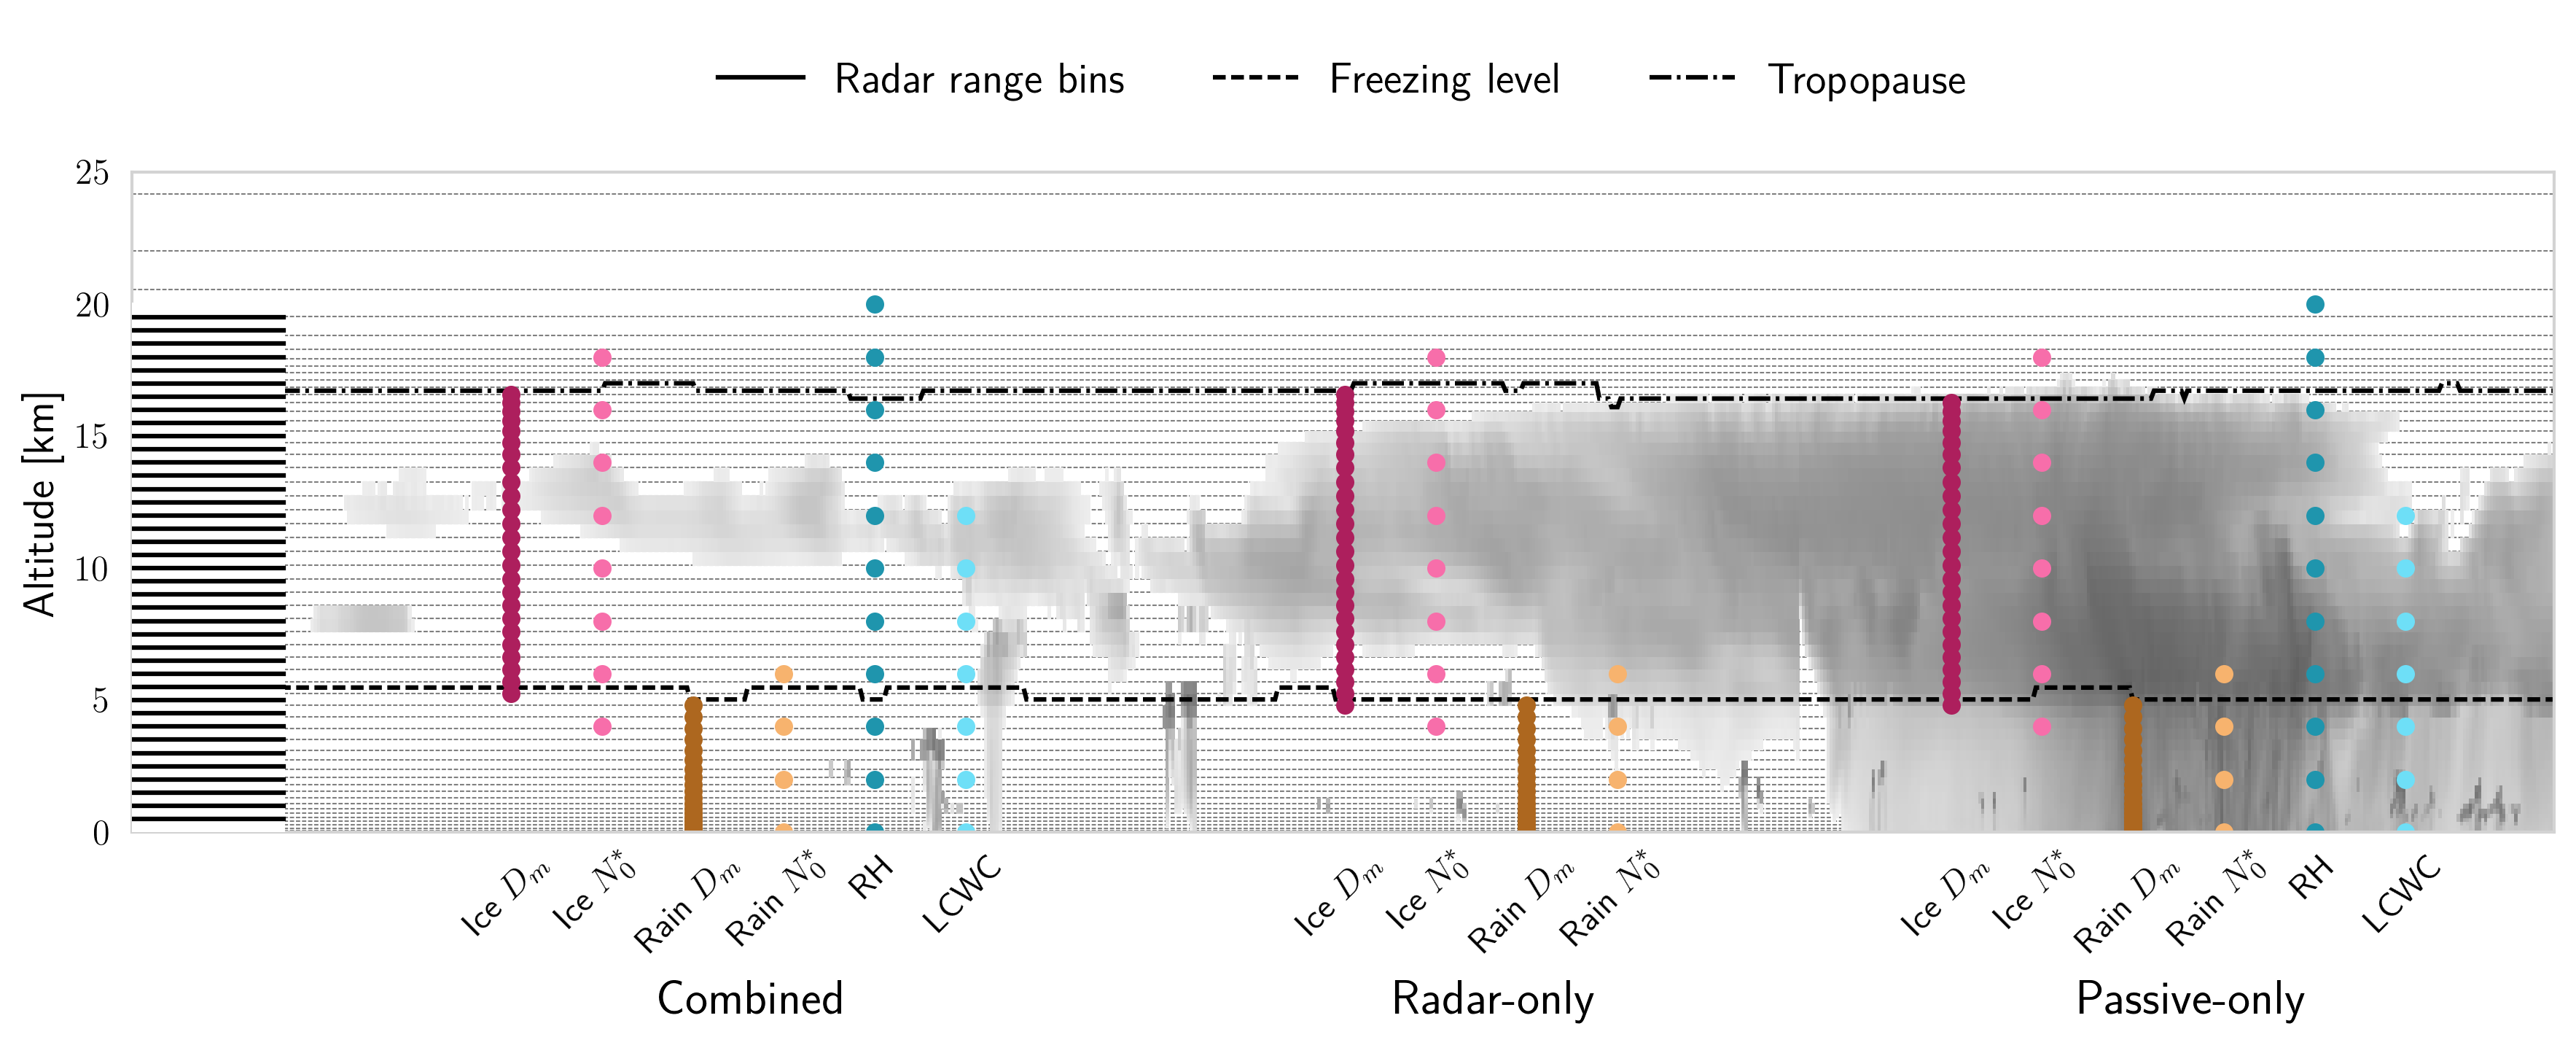
\includegraphics[width = 1.0\linewidth]{../plots/retrieval_sketch}
\caption{\DIFaddFL{Illustration of retrieval quantities and their respective retrieval
  grids. Grey, dashed lines in the background display the vertical grid of the
  GEM model. Black, solid lines on the left side display the range bins of the
  radar observations. Filled markers represent the retrieval grids of each
  retrieval quantity for the combined, radar-only and passive-only
  configurations of the retrieval algorithm.}}
\label{fig:retrieval_sketch}
\end{figure}

\DIFadd{The PSDs of frozen hydrometeors and rain }\DIFaddend are represented using the normalized
particle size distribution formalism proposed by \cite{delanoe05}. The PSD of a
hydrometeor species at a given \DIFdelbegin \DIFdel{height level is represented by a vertical and a horizontal scaling parameter, the }\DIFdelend \DIFaddbegin \DIFadd{altitude is modeled using a generalized gamma
distribution function with four parameters. The }\DIFaddend mass-weighted mean diameter
$D_m$\DIFaddbegin \DIFadd{, which scales the PSD along the size dimension, }\DIFaddend and the normalized number
density $N_0^*$\DIFdelbegin \DIFdel{. Alternative 
parametrizations using mass density and $D_m$ or the mass density and $N_0^*$
have been tested but no considerable effect on retrieval performance has been
observed.
}%DIFDELCMD < 

%DIFDELCMD < %%%
\DIFdel{The retrieval computes vertical profiles of the two scaling parameters $D_m$ and
$N_0^*$ for each of the two hydrometeor species. The remaining shape of each PSD
is described by the shape parameters $\alpha$ and $\beta$, not to
be confused with the parameters of the mass-size relationship shown in
Tab.~\ref{tab:species_parameters}. The shape parameters are set to fixed, species-specific
values. This principle is illustrated in Fig.~\ref{fig:psds_retrieval}.
The plot displays the a-priori-assumed shapes of the particle size distribution
of frozen and liquid hydrometeors. The retrieved horizontal and vertical scaling
parameters }\DIFdelend , \DIFdelbegin \DIFdel{$D_m$ and $N_0^*$, are used as units for the axes of the plot so
that }\DIFdelend \DIFaddbegin \DIFadd{which scales the particle concentration, are the two retrieved
degrees of freedom of the PSD. The other two parameters describe }\DIFaddend the shape of
the \DIFdelbegin \DIFdel{PSD becomes independent of the retrieved mass density and
number concentration. For frozen hydrometeors, the values of the shape parameters $\alpha$ and $\beta$ are chosen identical to }\DIFdelend \DIFaddbegin \DIFadd{normalized PSD. The same shape parameters as in }\DIFaddend version 3 of the
DARDAR-CLOUD product \citep{cazenave18} \DIFdelbegin \DIFdel{. For liquid hydrometeors, the shape
parameters are chosen so that they are equivalent to }\DIFdelend \DIFaddbegin \DIFadd{are chosen for frozen hydrometeors. For
rain, they are chosen to match }\DIFaddend the shape used \DIFdelbegin \DIFdel{by }\DIFdelend \DIFaddbegin \DIFadd{in }\DIFaddend the GEM model for rain drops.
\DIFdelbegin \DIFdel{All calculations involving particles size distributions
use the volume-equivalent diameter $D_\text{eq}$ as size variable.
}%DIFDELCMD < 

%DIFDELCMD < \begin{figure}
%DIFDELCMD < \centering
%DIFDELCMD < \includegraphics[width = 0.5\linewidth]{figures/fig03}
%DIFDELCMD < %%%
%DIFDELCMD < \caption{%
{%DIFAUXCMD
\DIFdelFL{PSD parametrizations for frozen and liquid hydrometeors
 used in the cloud retrieval.}}
%DIFAUXCMD
%DIFDELCMD < \label{fig:psds_retrieval}
%DIFDELCMD < \end{figure}
%DIFDELCMD < %%%
\DIFdelend 


The temperature-dependent a priori profile for $N_0^*$ \DIFdelbegin \DIFdel{of }\DIFdelend \DIFaddbegin \DIFadd{for }\DIFaddend frozen hydrometeors
is determined using the relation from \cite{delanoe14}
%
\begin{align}
N_0^* &= \exp \left ( -0.076586 \cdot (T - \DIFdelbegin \DIFdel{272.5}\DIFdelend \DIFaddbegin \DIFadd{273.15}\DIFaddend ) + 17.948 \right ),
\end{align}
%
where $T$ is in $\unit{K}$. The a priori profile \DIFdelbegin \DIFdel{for }\DIFdelend \DIFaddbegin \DIFadd{of }\DIFaddend $D_m$ for frozen
hydrometeors is chosen so that the a priori \DIFdelbegin \DIFdel{mass density }\DIFdelend \DIFaddbegin \DIFadd{IWC }\DIFaddend is equal to
$10^{-6}\ \unit{kg\ m^{-3}}$. For \DIFdelbegin \DIFdel{liquid hydrometeors}\DIFdelend \DIFaddbegin \DIFadd{rain}\DIFaddend , a fixed value for $N_0^*$ of
\DIFdelbegin \DIFdel{$10^6\ \unit{m^4}$ }\DIFdelend \DIFaddbegin \DIFadd{$10^6\ \unit{m^{-4}}$ }\DIFaddend is assumed and the a priori profile for $D_m$ is
determined similarly as for frozen hydrometeors.
\DIFdelbegin \DIFdel{Values of the mass-weighted mean diameter
$D_m$ for both hydrometeor species }\DIFdelend \DIFaddbegin 

\DIFadd{Since the $N_0^*$ parameters vary over several orders of magnitude they are
retrieved in $\log_{10}$-space for both frozen hydrometeors and rain. The $D_m$
parameters, in contrast, }\DIFaddend are retrieved in linear space\DIFdelbegin \DIFdel{, whereas the normalized number concentration parameter }\DIFdelend \DIFaddbegin \DIFadd{. Alternative
parametrizations using water content and $D_m$ or the water content and }\DIFaddend $N_0^*$
\DIFdelbegin \DIFdel{is retrieved in
$\text{log}_{10}$ space}\DIFdelend \DIFaddbegin \DIFadd{have been tested but no considerable effect on retrieval performance has been
observed}\DIFaddend . As additional constraints, the retrieval of frozen hydrometeors is
restricted to the region between the freezing \DIFdelbegin \DIFdel{layer and the tropopause, whereas the
retrieval of liquid }\DIFdelend \DIFaddbegin \DIFadd{level, here defined simply as the
$273.15\ \unit{K}$-isotherm, and the approximate altitude of tropopause. The
altitude of the tropopause is approximated as the first grid point at which the
lapse rate is negative and temperature below $220\ \unit{K}$. The retrieval of
rain }\DIFaddend hydrometeors is restricted to below the freezing \DIFdelbegin \DIFdel{layer. }%DIFDELCMD < 

%DIFDELCMD < %%%
\DIFdel{To further regularize the retrieval , $N_0^*$ for ice is retrieved at only 10
equally-spaced grid points between freezing layer and the tropopause. Similarly,
$D_m$ and }\DIFdelend \DIFaddbegin \DIFadd{level. The retrieval of
the }\DIFaddend $N_0^*$ \DIFdelbegin \DIFdel{for rain are retrieved at 10 respectively 4 points between surface and
freezing layer}\DIFdelend \DIFaddbegin \DIFadd{parameters is further regularized by retrieving them at reduced
vertical resolution of $2\ \unit{km}$}\DIFaddend . This was \DIFdelbegin \DIFdel{necessary to avoid }\DIFdelend \DIFaddbegin \DIFadd{found necessary to keep }\DIFaddend the
retrieval from getting stuck in spurious local minima. \DIFdelbegin \DIFdel{An approach similar to this one is also }\DIFdelend \DIFaddbegin \DIFadd{This resembles the
approach }\DIFaddend taken in the GPM combined precipitation retrievals \citep{grecu16}\DIFdelbegin \DIFdel{.
}\DIFdelend \DIFaddbegin \DIFadd{,
where the PSD parameter which scales the particle concentration is also
retrieved at reduced resolution.
}\DIFaddend 

\DIFdelbegin \DIFdel{Humidity in the atmospheric column is retrieved in units of relative humidity }\DIFdelend \DIFaddbegin \DIFadd{Relative humidity is retrieved }\DIFaddend at a vertical resolution of \DIFdelbegin \DIFdel{$1\ \unit{km}$}\DIFdelend \DIFaddbegin \DIFadd{$2\ \unit{km}$}\DIFaddend .
However, \DIFdelbegin \DIFdel{instead of retrieving relative
humidity directly , }\DIFdelend \DIFaddbegin \DIFadd{the values are not retrieved directly but instead }\DIFaddend an inverse
hyperbolic tangens transformation is applied to the relative humidity profile\DIFdelbegin \DIFdel{$\mathbf{\phi}$}\DIFdelend :
%
\begin{align}
x = \text{arctanh}(\DIFdelbegin \DIFdel{\frac{2 \mathbf{\phi}}{1.1} }\DIFdelend \DIFaddbegin \DIFadd{\frac{2 \text{RH}}{1.2} }\DIFaddend - 1.0)
\end{align}
%
The transformation restricts the retrieved relative humidity values to the range
\DIFdelbegin \DIFdel{of $[0.0, 1.1]$}\DIFdelend \DIFaddbegin \DIFadd{between $0$ and $120\%$}\DIFaddend . The a priori profile for relative humidity is \DIFdelbegin \DIFdel{arbitrarily chosen as
}\DIFdelend \DIFaddbegin \DIFadd{set to
}\DIFaddend %
\begin{align}
\DIFdelbegin \DIFdel{\phi}\DIFdelend \DIFaddbegin \DIFadd{\text{RH}}\DIFaddend (t) = \DIFdelbegin %DIFDELCMD < \begin{cases}
%DIFDELCMD <  0.7 &, 270\ \unit{K} < t \\
%DIFDELCMD <  0.7 - 0.01 \cdot (t - 270) & ,220 < t \leq  270\ \unit{K} \\
%DIFDELCMD <  0.2 \cdot (t - 270) & ,t < 220 \\
%DIFDELCMD <  \end{cases}%%%
\DIFdelend \DIFaddbegin \begin{cases}
 0.7 &, 270\ \unit{K} < t \\
 0.7 - 0.01 \cdot (270 -t) & ,220 < t \leq  270\ \unit{K} \\
 0.2 &,t < 220 \unit{K} \\
 \end{cases}\DIFaddend .
\end{align}
%
\DIFdelbegin \DIFdel{The retrieval of liquid cloud mass density, here referred to as liquid water
content (LWC), is performed at seven equally spaced altitude levels }\DIFdelend \DIFaddbegin \DIFadd{LCWC is retrieved at a resolution of $2\ \unit{km}$ but is restricted to the
region }\DIFaddend between the surface and the $230\ \unit{K}$ isotherm. In contrast to
frozen \DIFdelbegin \DIFdel{and liquid
hydrometeors , cloud water is modeled }\DIFdelend \DIFaddbegin \DIFadd{hydrometeors and rain, the PSD of liquid cloud droplets is not explicitly
resolved }\DIFaddend in the retrieval forward model\DIFdelbegin \DIFdel{to be purely absorbing using the absorption }\DIFdelend \DIFaddbegin \DIFadd{. Instead, liquid cloud droplets are
modeled as purely absorbing quantity using the }\DIFaddend model by \cite{liebe93} for
suspended liquid cloud droplets. \DIFdelbegin \DIFdel{Liquid cloud mass density }\DIFdelend \DIFaddbegin \DIFadd{Note that this is the case only for the
retrieval. For the simulated observations, liquid cloud droplets are
handled as any other hydrometeor species in the GEM model. LCWC }\DIFaddend is retrieved in
$\text{log}_{10}$-space and the a priori profile is set to a fixed value of
$10^{-6}\ \unit{kg\ m^{-3}}$ in the permitted region of the atmosphere.

The a priori distributions of the 6 retrieval quantities ($N_0^*$ and $D_m$ for
frozen and liquid hydrometeors, \DIFdelbegin \DIFdel{relative humidity $\phi$, cloud water}\DIFdelend \DIFaddbegin \DIFadd{RH, CLWC}\DIFaddend ) are assumed to be independent so that
the overall a priori covariance matrix $\mathbf{S}_a$ has block-diagonal
structure. Within each block, vertical correlations between the values of a
given retrieval quantity at different altitudes are assumed to be exponentially
decaying. Hence, the correlation of the values of retrieval quantity $q$ at
points $i$ and $j$ of the retrieval grid is computed as
%
\begin{align}
\left ( \mathbf{S}_{a,q} \right )_{i, j} &= \sigma_{q,i} \sigma_{q,j}
 \cdot \exp  \left ( -\frac{d(i, j)}{l_q} \right ),
\end{align}
%
where $\sigma_{q, i}$ is the a priori uncertainty assumed for retrieval
quantity $q$ at grid point $i$, $d(i, j)$ the distance between the grid
points and $l_q$ the quantity-specific correlation length. The assumed
a priori uncertainties and correlation lengths for the retrieval quantities
are summarized in Tab.~\ref{tab:a_priori}.

\begin{table}[h!]
\caption{A priori uncertainties and correlation
 lengths used in the retrieval.}
 \centering
\label{tab:a_priori}
    \DIFdelbeginFL %DIFDELCMD < \begin{tabular}{c|r|r}
%DIFDELCMD <      %%%
\DIFdelFL{Quantity $q$ }\DIFdelendFL \DIFaddbeginFL \begin{tabular}{ll|cc|cc|}
      \multicolumn{2}{c|}{Retrieval target}  & \multicolumn{2}{c|}{Combined / Radar only} & \multicolumn{2}{c}{Passive only}\\
      \DIFaddFL{Name }& \DIFaddFL{Retrieved quantity }&  \DIFaddFL{$\sigma_q$ }& \DIFaddFL{$l_q$ }[\DIFaddFL{km}] \DIFaddendFL & $\sigma_q$ & $l_q$ [km]\\
    \hline
\DIFdelbeginFL \DIFdelFL{$\log_{10}(N_{0, \text{frozen}}^*)$    }\DIFdelendFL \DIFaddbeginFL \DIFaddFL{Ice, $N_0^*$ }& \DIFaddFL{$\log_{10}(N_{0, \text{Ice}}^*)$ }& \DIFaddFL{$2$ }& \DIFaddFL{$2$ }\DIFaddendFL & $2$ &$5$ \\
\DIFdelbeginFL \DIFdelFL{$D_{m, \text{ice}}$               }\DIFdelendFL \DIFaddbeginFL \DIFaddFL{Ice, $D_m$ }&   \DIFaddFL{$\text{Ice }D_{m, \text{Ice}}$   }& \DIFaddFL{$300\ \unit{\mu m}$  }& \DIFaddFL{$2$ }\DIFaddendFL & $300\ \unit{\mu m}$          & $5$ \\
\DIFdelbeginFL \DIFdelFL{$\log_{10}(N_{0, \text{liquid}}^*)$    }\DIFdelendFL \DIFaddbeginFL \DIFaddFL{Rain, $N_0^*$ }\DIFaddendFL &    \DIFdelbeginFL \DIFdelFL{$2                      $ }\DIFdelendFL \DIFaddbeginFL \DIFaddFL{$\log_{10}(\text{Rain } N_{0}^*)$ }\DIFaddendFL & $2$ \DIFdelbeginFL %DIFDELCMD < \\
%DIFDELCMD <     %%%
\DIFdelFL{$D_{m, \text{liquid}}$            }\DIFdelendFL & \DIFdelbeginFL \DIFdelFL{$500\ \unit{\mu m}$           }\DIFdelendFL \DIFaddbeginFL \DIFaddFL{$2$ }\DIFaddendFL & $2$ \DIFaddbeginFL &\DIFaddFL{$5$ }\DIFaddendFL \\
\DIFdelbeginFL \DIFdelFL{$\text{arctanh}(\frac{2 \cdot \phi}{1.1} - 1.0)$ }\DIFdelendFL \DIFaddbeginFL \DIFaddFL{Rain, $D_m$ }&  \DIFaddFL{$D_{m, \text{Rain}}$   }& \DIFaddFL{$300\ \unit{\mu m}$  }\DIFaddendFL & $2$ & \DIFaddbeginFL \DIFaddFL{$300\ \unit{\mu m}$          }& \DIFaddFL{$5$ }\\
\DIFaddFL{Relative humidity (RH) }& \DIFaddFL{$\text{arctanh}(\frac{2 \cdot \text{RH}}{1.2} - 1.0)$ }& \DIFaddFL{$0.5^{*}$ }& \DIFaddFL{$2^{*}$ }& \DIFaddFL{$0.5$ }& \DIFaddendFL $2$ \\
\DIFdelbeginFL \DIFdelFL{$\log_{10}(m_\text{liquid cloud}) $ }\DIFdelendFL \DIFaddbeginFL \DIFaddFL{Cloud liquid water content (CLWC) }& \DIFaddFL{$\log_{10}(\text{CLWC}) $ }& \DIFaddFL{$1^{*}$ }& \DIFaddFL{$2^{*}$  }\DIFaddendFL & $1$ & $2$ \\
\DIFaddbeginFL \multicolumn{6}{l}{$^*$: Not retrieved in radar-only retrieval}
    \DIFaddendFL \end{tabular}
\end{table}

\DIFdelbegin \DIFdel{As baselines for the assessment of the combined }\DIFdelend \DIFaddbegin \DIFadd{The radar-only version of the retrieval is similar to the combined version
except that RH and LCWC are not retrieved. Instead, perfect knowledge of the
true RH profile is assumed while LCWC is neglected. In addition to a two-moment
radar-only }\DIFaddend retrieval, also a \DIFdelbegin \DIFdel{radar-only and a passive only-retrieval are performed.
The radar-only retrievaluses the same
implementation as }\DIFdelend \DIFaddbegin \DIFadd{one-moment version (M1), which retrieves only the
$D_m$ parameter has been tested. For completeness, retrieval results for IWC
will be reported also for the M1 version. However, to allow for better comparison
with the combined and passive-only retrieval, is the remainder of this work
only the two-moment version is considered.
}

\DIFadd{For the passive-only retrieval, the retrieval quantities and grids are the same
as for }\DIFaddend the combined retrieval\DIFdelbegin \DIFdel{, but only retrieves frozen and liquid
hydrometeors.
For the radar-only retrieval, perfect knowledge of the atmospheric
humidity profile is assumed but liquid cloud is ignored in the }\DIFdelend \DIFaddbegin \DIFadd{. However, higher correlations lengths are assumed,
which are shown in Tab.~\ref{tab:a_priori}
}

\subsubsection{\DIFadd{Representation of ice particle shape}}
\label{sec:method:partilce_models}

\DIFadd{A major difficulty for cloud retrievals is that the observations do not provide
sufficient information to distinguish different hydrometeor species. In the
proposed retrieval algorithm, this difficulty is overcome by representing frozen
hydrometeors using only a single hydrometeor species. This, however, poses the
problem of finding a suitable representation of frozen hydrometeors that can
capture variability of the four frozen hydrometeor species in the model and
ideally also real ice hydrometeors.
}

\DIFadd{In the model scenario considered here, the differences between hydrometeor
species are mostly due to their different concentrations, sizes (c.f.
Fig.~\ref{fig:gem_psds}) and shape. Since two parameters of the PSD of frozen
hydrometeor species are retrieved, the retrieval can represent differences
between the PSDs of the different hydrometeor species. To capture the
variability in particle shape, it is possible to use habit mixes that combine
crystal shapes at small particle sizes with aggregate shapes at larger sizes.
This provides the retrieval with flexibility to represent differences between
cloud ice on the one hand and snow, graupel and hail hydrometeors on the other.
}

\DIFadd{It is clear that even with this configuration, the simplified }\DIFaddend retrieval forward
model \DIFdelbegin \DIFdel{.
}%DIFDELCMD < 

%DIFDELCMD < %%%
\DIFdel{The setup and retrieval quantities of the passive-only retrieval are similar to the combined retrieval, with the only difference being that frozen and liquid
hydrometeors are retrieved at reduced resolution. For ice, }\DIFdelend \DIFaddbegin \DIFadd{will not be able to represent every possible configuration of mixes of the
four ice hydrometeor species in the GEM model. In particular, it remains unclear
which particle shape should be used to best represent this mixture. We therefore
choose a set consisting of multiple particle shapes and habit mixes, which will
be used in the retrieval to study the impact of the choice of the particle shape
on the retrieval results. The selected particles are listed in
Tab.~\ref{tab:particle_properties}. Three of them, GEM Cloud Ice, GEM Snow, and
GEM Graupel, correspond to the shapes present in the GEM model scenes. The GEM
Snow and Graupel habits were mixed with crystal shapes to ensure that they cover
sizes down to around $10\ \unit{\mu m}$. In addition to this, two of the habit
mixes distributed with the ARTS SSDB, Large Plate Aggregate and Large Column
Aggregate, are added to the selection to increase the coverage of the range of
scattering properties in the database. Fig.~\ref{fig:particle_properties}
provides an overview of the bulk radiometric properties with respect to bulk
mass of the selected particles computed for three different values of the
}\DIFaddend $N_0^*$ \DIFdelbegin \DIFdel{is retrieved
at three equally spaced grid points between freezing layer and troposphere, while
$D_m$ is retrieved at five. For liquid hydormeteors, the retrieval grids for $N_0^*$ and $D_m$ are reduced to two equally spaced points between surface and freezing layer. Relative humidity is retrieved at
a vertical resolution of $2\ \unit{km}$}\DIFdelend \DIFaddbegin \DIFadd{parameter of the PSD. For high values of $N_0^*$, which are typical for
cloud ice, the radiometric properties of particle shapes differ only for large
masses at the two highest frequencies considered. For low $N_0^*$ values, which
are more typical for snow, the particles' properties differ considerably at all
masses and frequencies. The dominating behavior is that the Large Column
Aggregate, Large Plate Aggregate and GEM Snow are less efficient in their
interaction with radiation. In contrast to that, GEM Graupel, Gem Hail and GEM
Cloud Ice are more efficient. However, for the lowest $N_0^*$ values at
the two highest frequencies the relative ordering of the efficiencies is
actually reversed and increases with increasing mass}\DIFaddend .


\DIFaddbegin \begin{table}
  \centering
  \caption{\DIFaddFL{Particle mixes used to represent ice hydrometeors used in the
    retrieval}}
  \begin{tabular}{l|l|rr|rr}
    \multicolumn{1}{c|}{Name} & \multicolumn{1}{c|}{Shapes used} &
    \multicolumn{2}{c|}{Size range} & \multicolumn{2}{c}{Mass size relationship}
    \\
    & \DIFaddFL{Name (ID) }&\DIFaddFL{$D_{\text{eq}, \text{ min}}\ [\unit{\mu m}$}] &
    \DIFaddFL{$D_{\text{eq}, \text{ max}}\ [\unit{\mu m}]$ }&\hfill
    \DIFaddFL{$\alpha\ [\unit{kg\ m^{-3}}]$ }& \hfill \DIFaddFL{$\beta\ [\ ]$ }\\
    \hline \hline %DIF >  GEM
    \DIFaddFL{CloudIce }& \DIFaddFL{GEM CloudIce (11) }& \DIFaddFL{$10\ $ }& \DIFaddFL{$3000\ $ }& \hfill \DIFaddFL{440 }& \hfill \DIFaddFL{3 }\\
    %DIF > 
    %DIF > 
    %DIF >  GEM Snow
    %DIF > 
    \hline \DIFaddFL{GEM Snow }& \DIFaddFL{Evans Snow Aggregate (1) }& \DIFaddFL{$10\ $ }& \DIFaddFL{$127\ $ }& \hfill \DIFaddFL{440 }&
    \hfill \DIFaddFL{3 }\\ & \DIFaddFL{GEM Snow (32) }& \DIFaddFL{$107\ $ }& \DIFaddFL{$5000\ $ }& \hfill \DIFaddFL{24 }& \hfill \DIFaddFL{2.86
    }\\
    %DIF > 
    %DIF >  Gem Graupel
    %DIF > 
    \hline \DIFaddFL{GEM Graupel }& \DIFaddFL{8-Column Aggregate(8) }& \DIFaddFL{$10\ $ }& \DIFaddFL{$179\ $ }& \hfill \DIFaddFL{65 }&
    \hfill \DIFaddFL{3 }\\ & \DIFaddFL{GEM Graupel (33) }& \DIFaddFL{$107\ $ }& \DIFaddFL{$5000\ $ }& \hfill \DIFaddFL{170 }& \hfill
    \DIFaddFL{2.96 }\\
    %DIF > 
    %DIF >  Large Plate Aggregate
    %DIF > 
    \hline \DIFaddFL{Large Plate Aggregate }& \DIFaddFL{Thick Plate (15) }& \DIFaddFL{$16\ $ }& \DIFaddFL{$200\ $ }& \hfill
    \DIFaddFL{110 }& \hfill \DIFaddFL{3 }\\ & \DIFaddFL{Large Plate Aggregate (33) }& \DIFaddFL{$160\ $ }& \DIFaddFL{$3021\ $ }& \hfill
    \DIFaddFL{0.21 }& \hfill \DIFaddFL{2.26 }\\
    %DIF > 
    %DIF >  Large Column Aggregate
    %DIF > 
    \hline \DIFaddFL{Large Column Aggregate }& \DIFaddFL{Block Column (12) }& \DIFaddFL{$10\ $ }& \DIFaddFL{$200\ $ }&
    \hfill \DIFaddFL{110 }& \hfill \DIFaddFL{3 }\\ & \DIFaddFL{Large Column Aggregate (22) }& \DIFaddFL{$160\ $ }& \DIFaddFL{$3021\ $
    }& \hfill \DIFaddFL{0.25 }& \hfill \DIFaddFL{2.43 }\\
  \end{tabular}
  \label{tab:particle_properties}
\end{table}

\begin{figure}
  \centering
  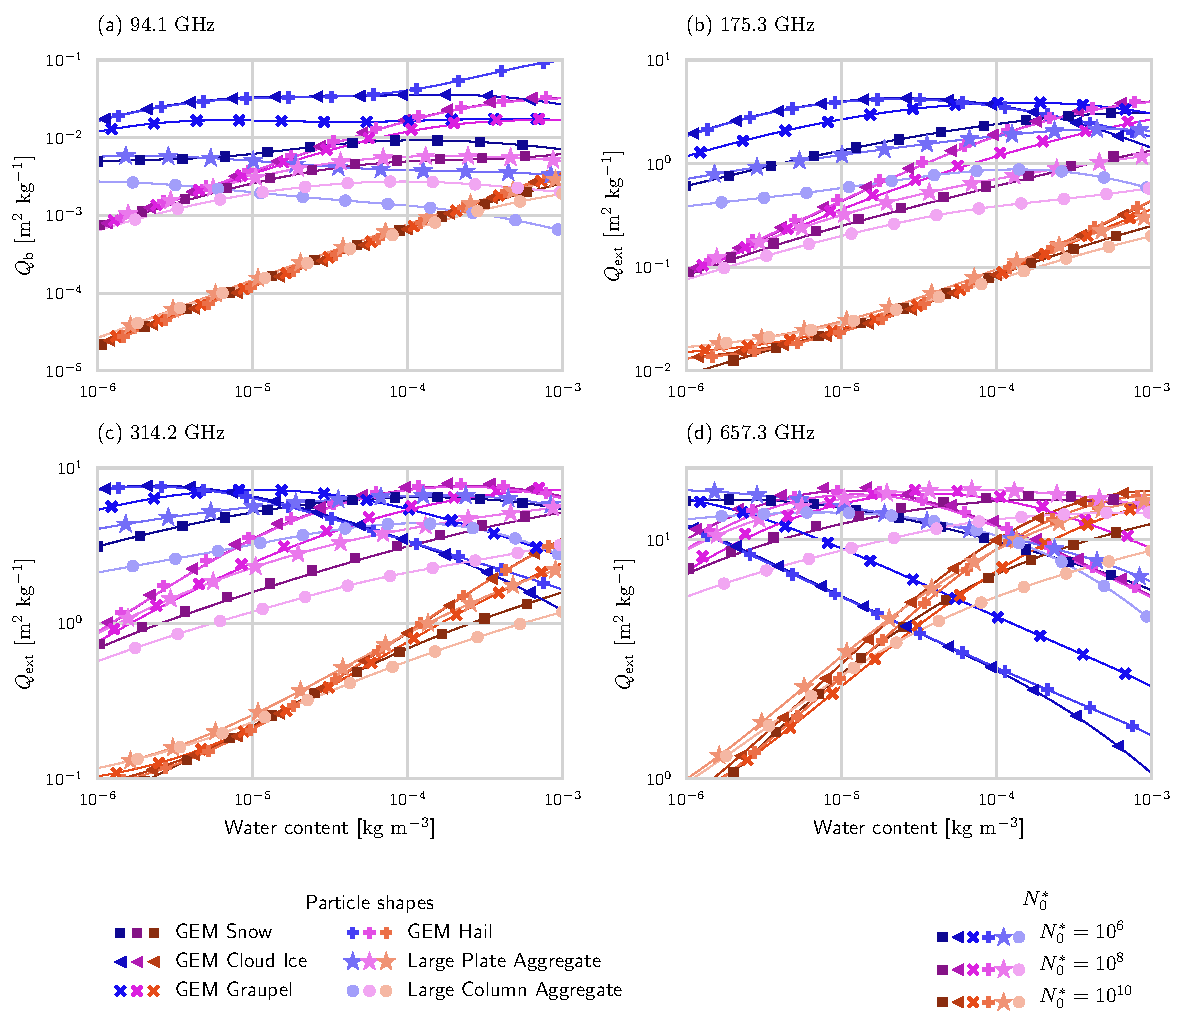
\includegraphics[width=0.8\textwidth]{../plots/particle_properties_d14}
  \caption{\DIFaddFL{Bulk backscattering efficiency $Q_b$ at $94.1\ \unit{GHz}$ (Panel
    (a)) and bulk extinction efficiencies $Q_{e}$ at frequencies
    $175.3\ \unit{GHz}$ (Panel (b)), $314.2\ \unit{GHz}$ (Panel (c)) and
    $657.3\ \unit{GHz}$ for the particle models used in the simulated
    observations and the retrieval. Bulk properties are computed for different
    values of the $N_0^*$ parameter of the PSD, which is proportional to the
    particle number concentration for a given bulk mass.}}
  \label{fig:particle_properties}
\end{figure}

\DIFaddend \section{Results}
\label{sec:results}

The first part of this section presents results from a numerical experiment that
investigates the complementary information content of the active and passive
microwave observations. Results of the combined and the \DIFdelbegin \DIFdel{baseline }\DIFdelend \DIFaddbegin \DIFadd{single-instrument
}\DIFaddend retrievals applied to the reference cloud scenes are presented in the remaining
part\DIFdelbegin \DIFdel{of this section}\DIFdelend .

\subsection{Complementary information content}
\label{sec:simple_cloud}

A fundamental question regarding the benefit of combining two remote sensing
observations in a retrieval is to what extent the observations contain
non-redundant information. The degree of non-redundancy in the combined
observations is what we refer to here as complementary information content. \DIFaddbegin \DIFadd{We
are thus interested here in the information that cannot be provided by either of
the instruments alone. Because of this, we do not consider the higher resolution
achieved by adding radar observations to passive ones as complementary
information, since the radar alone can provide the increased resolution.
}

\DIFaddend In order to explore \DIFdelbegin \DIFdel{this }\DIFdelend \DIFaddbegin \DIFadd{the }\DIFaddend complementary information content in the radar and
radiometer observations, an idealized, homogeneous cloud layer with a thickness
of \DIFdelbegin \DIFdel{$4\ \unit{km}$ }\DIFdelend \DIFaddbegin \DIFadd{$5\ \unit{km}$ }\DIFaddend located at an altitude of $10\ \unit{km}$ in a tropical
atmosphere is considered. The cloud is assumed to consist of a single species of
frozen hydrometeors represented using the PSD parametrization which is also used
in the retrieval and described in Sec.~\DIFdelbegin \DIFdel{\ref{sec:method:fowardmodel}}\DIFdelend \DIFaddbegin \DIFadd{\ref{sec:method:state_space}}\DIFaddend . As particle
model, the \DIFdelbegin \DIFdel{8-ColumnAggregate }\DIFdelend \DIFaddbegin \DIFadd{8-Column Aggregate }\DIFaddend (ID 8) from the ARTS SSDB is used.

The question that is addressed here is whether the combination of active and
passive observations is able to constrain both the \DIFdelbegin \DIFdel{horizontal and the
vertical scaling factors of the PSD }\DIFdelend \DIFaddbegin \DIFadd{size and concentration }\DIFaddend of the
ice particles in the cloud. To investigate this, the $N_0^*$ and $D_m$
parameters of the homogeneous cloud layer are varied and observations of the
cloud \DIFdelbegin \DIFdel{layer }\DIFdelend are simulated. \DIFdelbegin \DIFdel{Figure
\ref{fig:contours} displays the simulated passive cloud signal , i.e. the
brightness
temperature difference between clear sky and cloudy sky simulation, as filled
contours for a selection of channels of the MWI and ICI sensors. For given
values of $N_0^*$ and $D_m$, the corresponding ice mass density is given by
the relation
}\begin{eqnarray*}
\DIFdel{m = \frac{\pi \rho}{4 ^ 4}N_0^* D_m^4.
}\end{eqnarray*}
%DIFAUXCMD
\DIFdel{In the figure, the cloud signal is displayed in
$D_m$-mass density space and
thus shows how the measured passive cloud signal varies with the horizontal and
vertical scaling parameters of the PSD.
Overlaid onto }\DIFdelend \DIFaddbegin \DIFadd{The cloud signal in the radiometer observations is the
difference between the cloudy- and clear-sky brightness temperatures ($\Delta
T_B$). The signal in the active observations is here defined as the maximum in
the measured profile of radar reflectivity $\text{dBZ}_\text{max}$.
Figure~\ref{fig:contours} displays }\DIFaddend the contours of \DIFdelbegin \DIFdel{the
passive cloud signal are the isolines of the maximum radar reflectivity returned
from the cloud}\DIFdelend \DIFaddbegin \DIFadd{$\Delta T_B$ and
$\text{dBZ}_\text{max}$ with respect to $D_m$ and the clouds water content,
which is proportional to $N_0^*$:
}\begin{align}
\DIFadd{m = \frac{\pi \rho}{4 ^ 4}N_0^* D_m^4,
}\end{align}
\DIFadd{with $\rho$ the density of ice}\DIFaddend .

\begin{figure}
\centering
\DIFdelbeginFL %DIFDELCMD < \includegraphics[width = 0.8\textwidth]{figures/fig04}
%DIFDELCMD < %%%
\DIFdelendFL \DIFaddbeginFL \includegraphics[width = 1.0\textwidth]{figures/fig04}
\DIFaddendFL \caption{Simulated observations of a homogeneous, $5\ \unit{km}$ thick cloud
  layer with varying water content $m$ and mass-weighted mean diameter $D_m$.
  The panels display the maximum radar reflectivity in dBZ
  \DIFaddbeginFL \DIFaddFL{($\text{dBZ}_\text{max}$) }\DIFaddendFL overlaid onto the cloud signal \DIFaddbeginFL \DIFaddFL{($\Delta T_B$)
  }\DIFaddendFL measured by selected radiometer channels of the MWI (first row) and ICI
  radiometers (second row).}
\label{fig:contours}
\end{figure}

The contours of \DIFdelbegin \DIFdel{the measured active and passive cloud signals }\DIFdelend \DIFaddbegin \DIFadd{$\Delta T_B$ and $\text{dBZ}_\text{max}$  }\DIFaddend show the ambiguity
of the single-instrument \DIFdelbegin \DIFdel{measurements }\DIFdelend \DIFaddbegin \DIFadd{observations }\DIFaddend with respect to the parameters of the PSD:
Along these contours the signal does not change, while the cloud composition
does. A necessary condition for a combined cloud retrieval to be able to resolve
this ambiguity is that the contours of the active and passive signals cross each
other. The panels in Fig.~\ref{fig:contours} thus provide an indication to what
extent the information in the radar measurement and the corresponding passive
radiometer channel provide complementary information on the parameters of the
PSD. Considering the panels corresponding to the MWI channels, the results show
that the observations contain complementary information only for very dense
clouds consisting of very large particles. In contrast to that, the ICI
observations exhibit crossing contours already at lower $m$ and $D_m$ values,
indicating that the complementary information content in these observations is
higher for less dense clouds consisting of smaller particles.

\subsection{Retrieval results}

To assess the performance of the combined cloud retrieval, the developed
algorithm has been applied to the two designated cloud scenes. The same
retrievals have been performed with a radar-only and a passive-only version of
the algorithm to serve as baselines for the combined retrieval. Each retrieval
was performed multiple times using \DIFaddbegin \DIFadd{the }\DIFaddend different ice particle models \DIFdelbegin \DIFdel{. The tested
particle shapes are listed together with the corresponding mass size relations
and ARTS SSDB identifier }\DIFdelend \DIFaddbegin \DIFadd{listed }\DIFaddend in
Tab.~\DIFdelbegin \DIFdel{\ref{tab:particles_retrieval}}\DIFdelend \DIFaddbegin \DIFadd{\ref{tab:particle_properties}}\DIFaddend . Since the results for both test scenes are
qualitatively similar, \DIFdelbegin \DIFdel{not all analyses are shown for both scenes. Instead, these }\DIFdelend \DIFaddbegin \DIFadd{results from the second scene are provided in the
appendix. Complete results for all retrieval quantities, both scenes and all
tested particle shapes }\DIFaddend are provided as \DIFdelbegin \DIFdel{a }\DIFdelend digital supplement to this article.

\DIFdelbegin %DIFDELCMD < \begin{table}
%DIFDELCMD <   \centering
%DIFDELCMD <   %%%
%DIFDELCMD < \caption{%
{%DIFAUXCMD
\DIFdelFL{Particle model name, ARTS scattering database ID and parameters
    $\alpha, \beta$ of the mass-size relationships of the particle habits used
    in the retrieval.}}
  %DIFAUXCMD
%DIFDELCMD < \begin{tabular}{l|c|c|c}
%DIFDELCMD <     %%%
\DIFdelFL{Name }%DIFDELCMD < & %%%
\DIFdelFL{ID }%DIFDELCMD < & %%%
\DIFdelFL{$\alpha$ }%DIFDELCMD < & %%%
\DIFdelFL{$\beta$ }%DIFDELCMD < \\
%DIFDELCMD <     \hline
%DIFDELCMD <     %%%
\DIFdelFL{GemCloudIce         }%DIFDELCMD < & %%%
\DIFdelFL{31  }%DIFDELCMD < & %%%
\DIFdelFL{440      }%DIFDELCMD < & %%%
\DIFdelFL{3 }%DIFDELCMD < \\
%DIFDELCMD <     %%%
\DIFdelFL{GemSnow             }%DIFDELCMD < & %%%
\DIFdelFL{32  }%DIFDELCMD < & %%%
\DIFdelFL{24.0072  }%DIFDELCMD < & %%%
\DIFdelFL{2.8571 }%DIFDELCMD < \\
%DIFDELCMD <     %%%
\DIFdelFL{GemGraupel          }%DIFDELCMD < & %%%
\DIFdelFL{33  }%DIFDELCMD < & %%%
\DIFdelFL{172.7527 }%DIFDELCMD < & %%%
\DIFdelFL{2.9646 }%DIFDELCMD < \\
%DIFDELCMD <     %%%
\DIFdelFL{8-ColumnAggregate   }%DIFDELCMD < &  %%%
\DIFdelFL{8  }%DIFDELCMD < & %%%
\DIFdelFL{65.4480  }%DIFDELCMD < & %%%
\DIFdelFL{3      }%DIFDELCMD < \\
%DIFDELCMD <     %%%
\DIFdelFL{PlateType1          }%DIFDELCMD < &  %%%
\DIFdelFL{9  }%DIFDELCMD < & %%%
\DIFdelFL{2.4770   }%DIFDELCMD < & %%%
\DIFdelFL{0.7570 }%DIFDELCMD < \\
%DIFDELCMD <     %%%
\DIFdelFL{LargePlateAggregate }%DIFDELCMD < &  %%%
\DIFdelFL{20 }%DIFDELCMD < & %%%
\DIFdelFL{2.2571   }%DIFDELCMD < & %%%
\DIFdelFL{0.2085 }%DIFDELCMD < \\
%DIFDELCMD <   \end{tabular}
%DIFDELCMD <   \label{tab:particles_retrieval}
%DIFDELCMD < \end{table}
%DIFDELCMD < 

%DIFDELCMD < %%%
\DIFdelend The forward-simulated observations that were generated to test the retrievals
are shown for the first test scene in Fig.~\ref{fig:observations_a}. Independent
Gaussian noise with standard deviations according to sensor specifications has
been added to the simulated observations to account for sensor noise. It is
important to note \DIFdelbegin \DIFdel{, }\DIFdelend that the simulated observations which are used to test the
retrieval assume different microphysics than what is assumed in the retrieval\DIFdelbegin \DIFdel{:
}\DIFdelend \DIFaddbegin \DIFadd{.
}\DIFaddend The synthetic observations are computed using the six hydrometeor classes from
the GEM model, while the retrieval forward model assumes only two classes of
hydrometeors.

\begin{figure}
\centering \includegraphics[width = 0.8\textwidth]{figures/fig05}
\caption{Total hydrometeor content (HMC) and simulated observations for the
  first test scene. Panel (a) displays the total hydrometeor content in the
  scene, i.e. the sum of the \DIFdelbeginFL \DIFdelFL{mass densities }\DIFdelendFL \DIFaddbeginFL \DIFaddFL{water content }\DIFaddendFL of all hydrometeor species of the GEM
  model. Panel (b) shows the simulated radar reflectivities. Panel (c) displays
  the simulated brightness temperatures for a selection of the channels of the
  MWI and ICI radiometers.}
\label{fig:observations_a}
\end{figure}

\subsubsection{Mass concentrations}

\DIFdelbegin \DIFdel{To provide an overview over how well the different retrieval methods are able to
reproduce the cloud structures in the test scene, the retrieved ice water content (IWC) }\DIFdelend \DIFaddbegin \DIFadd{Results of the retrieved water content obtained using the Large Plate Aggregate
particle mode }\DIFaddend for the first test scene \DIFdelbegin \DIFdel{is shown in
Figure \ref{fig:results_a}. IWC }\DIFdelend \DIFaddbegin \DIFadd{are displayed in
Fig.~\ref{fig:results_a}. The reference water content }\DIFaddend is defined here as the sum
of the \DIFdelbegin \DIFdel{mass densities of all frozen hydrometeor
species. This means that the reference IWC is the sum }\DIFdelend \DIFaddbegin \DIFadd{masses }\DIFaddend of the four frozen hydrometeor species \DIFdelbegin \DIFdel{represented }\DIFdelend in the GEM model \DIFdelbegin \DIFdel{, whereas the retrieved IWC is
simply the mass density of the single frozen hydrometeor species assumed in the
retrieval.
The results shown here were obtained using the LargePlateAggregate as
particle model, which was found to be one of the best performing particle
models.
}%DIFDELCMD < 

%DIFDELCMD < %%%
\DIFdelend \DIFaddbegin \DIFadd{scenes.
}

\DIFadd{The $\chi^2_y$ values for the three retrieval configurations, displayed in }\DIFaddend Panel
(a)\DIFdelbegin \DIFdel{of the figure displays the $\chi^2_y$ value (normalized by the
dimension of the measurement space) for each profile in the scene. A high value
of $\chi^2_y$ indicates that the retrieved state is not consistent with the
input observations. The $\chi^2_y$ value for }\DIFdelend \DIFaddbegin \DIFadd{, gives an indication of how well the retrievals were able to fit the
observations. For }\DIFaddend the radar-only retrieval\DIFdelbegin \DIFdel{is
remarkably low throughout most }\DIFdelend \DIFaddbegin \DIFadd{, the values are much smaller than 1
for most parts }\DIFaddend of the scene\DIFdelbegin \DIFdel{. This may indicate that the
retrieval is insufficiently regularized, allowing it to fit the noise in the observations. The }\DIFdelend \DIFaddbegin \DIFadd{, while for the }\DIFaddend passive-only and combined retrieval
\DIFdelbegin \DIFdel{, on the contrary, have a
normalized $\chi^2_y$ value around 1 over most of the scene. Since the presented
values are normalized, the value 1 corresponds to }\DIFdelend \DIFaddbegin \DIFadd{they are around }\DIFaddend the expected value of \DIFdelbegin \DIFdel{the
approximated chi-square distribution of $\chi^2_y$. All three retrievals exhibit
a region of elevated $\chi^2_y$ values near the core of the convective system.
In particular the high values of }\DIFdelend \DIFaddbegin \DIFadd{1. This indicates that }\DIFaddend the passive-only
and combined \DIFdelbegin \DIFdel{retrievals
indicate that the retrieval was not able to find a good }\DIFdelend \DIFaddbegin \DIFadd{retrieval achieve the expected }\DIFaddend fit to the observations \DIFdelbegin \DIFdel{here.
}%DIFDELCMD < 

%DIFDELCMD < %%%
\DIFdel{Panel (b) displays the
retrieved column-integrated IWC, the ice water path
(IWP). The IWP is given in $\unit{dB}$ relative to the
reference IWP since, owing to the high dynamic range of the reference values, }\DIFdelend \DIFaddbegin \DIFadd{but that the
radar-only retrieval actually overfits the observations. The exception is }\DIFaddend the
\DIFdelbegin \DIFdel{curves could
otherwise not be distinguished.
Although all methods reproduce the reference
IWP fairly well, the combined retrieval yields the best overall agreement with
}\DIFdelend \DIFaddbegin \DIFadd{region around $3^\circ\ N$, where the cloud is particularly thick and consists
of a mix of different hydrometeor types. Here, especially the passive-only
retrieval has problems fitting the observations.
}

\DIFadd{In terms of IWP, all methods provide fairly good estimates of }\DIFaddend the reference
values. \DIFdelbegin \DIFdel{Exceptions are the regions of high $\chi^2_y$ values where
the retrieval failed to find a good fit to the observations.
}%DIFDELCMD < 

%DIFDELCMD < %%%
\DIFdel{Panel (c) shows the IWC field retrieved using the passive-only retrieval
.
Despite a certain resemblance in the overall structure between the retrieved and
reference IWCfield, the results do not reproduce }\DIFdelend \DIFaddbegin \DIFadd{The combined retrieval consistently yields the smallest deviations.
Larger differences between the methods are observed when comparing the retrieval
results in terms of IWC. While }\DIFaddend the vertical structure of the cloud \DIFdelbegin \DIFdel{very well. It should be noted, however, that the displayed mass-density
range extends below the sensitivity limit of the passive-only observations
around $10^{-5}\ \unit{kg\ m^{-3}}$ (c.f. Fig. ~\ref{fig:contours}), which explains
the smeared-out appearance of the
results to some extent.
}%DIFDELCMD < 

%DIFDELCMD < %%%
\DIFdel{The }\DIFdelend \DIFaddbegin \DIFadd{is captured
only very roughly by the passive retrieval, it is better resolved by the
}\DIFaddend radar-only \DIFdelbegin \DIFdel{results, shown in panel (d), reproduce the vertical structure of
the cloud well. Nonetheless, when compared to the reference IWC field, certain
discrepancies are visible: The }\DIFdelend \DIFaddbegin \DIFadd{and the combined retrieval. On closer inspection, however, it becomes
evident that the }\DIFaddend radar-only retrieval \DIFdelbegin \DIFdel{tends to overestimate the
mass density at the bottom }\DIFdelend \DIFaddbegin \DIFadd{deviates systematically from the reference
IWC in specific regions }\DIFaddend of the cloud\DIFdelbegin \DIFdel{and underestimate the mass
concentrations at the top }\DIFdelend \DIFaddbegin \DIFadd{, such as for example the upper part }\DIFaddend of the
cloud \DIFdelbegin \DIFdel{.
}%DIFDELCMD < 

%DIFDELCMD < %%%
\DIFdel{The results of the combined retrieval are displayed in panel (e). Although some
artifacts are clearly visible in the
retrieved IWC field, the retrieval
reproduces the vertical structure well. In particular, }\DIFdelend \DIFaddbegin \DIFadd{between $0^\circ N$ and $2^\circ N$. These deviations are corrected in the
results from }\DIFaddend the combined retrieval\DIFdelbegin \DIFdel{succeeds to correct some of the systematic deviations of the radar-only
retrieval : The mass density at cloud base is reduced and increased at cloud top}\DIFdelend \DIFaddbegin \DIFadd{, although certain retrieval artifacts are
visible}\DIFaddend .

\begin{figure}
\centering
\DIFdelbeginFL %DIFDELCMD < \includegraphics[width = 0.8\textwidth]{figures/fig06}
%DIFDELCMD < %%%
\DIFdelendFL \DIFaddbeginFL 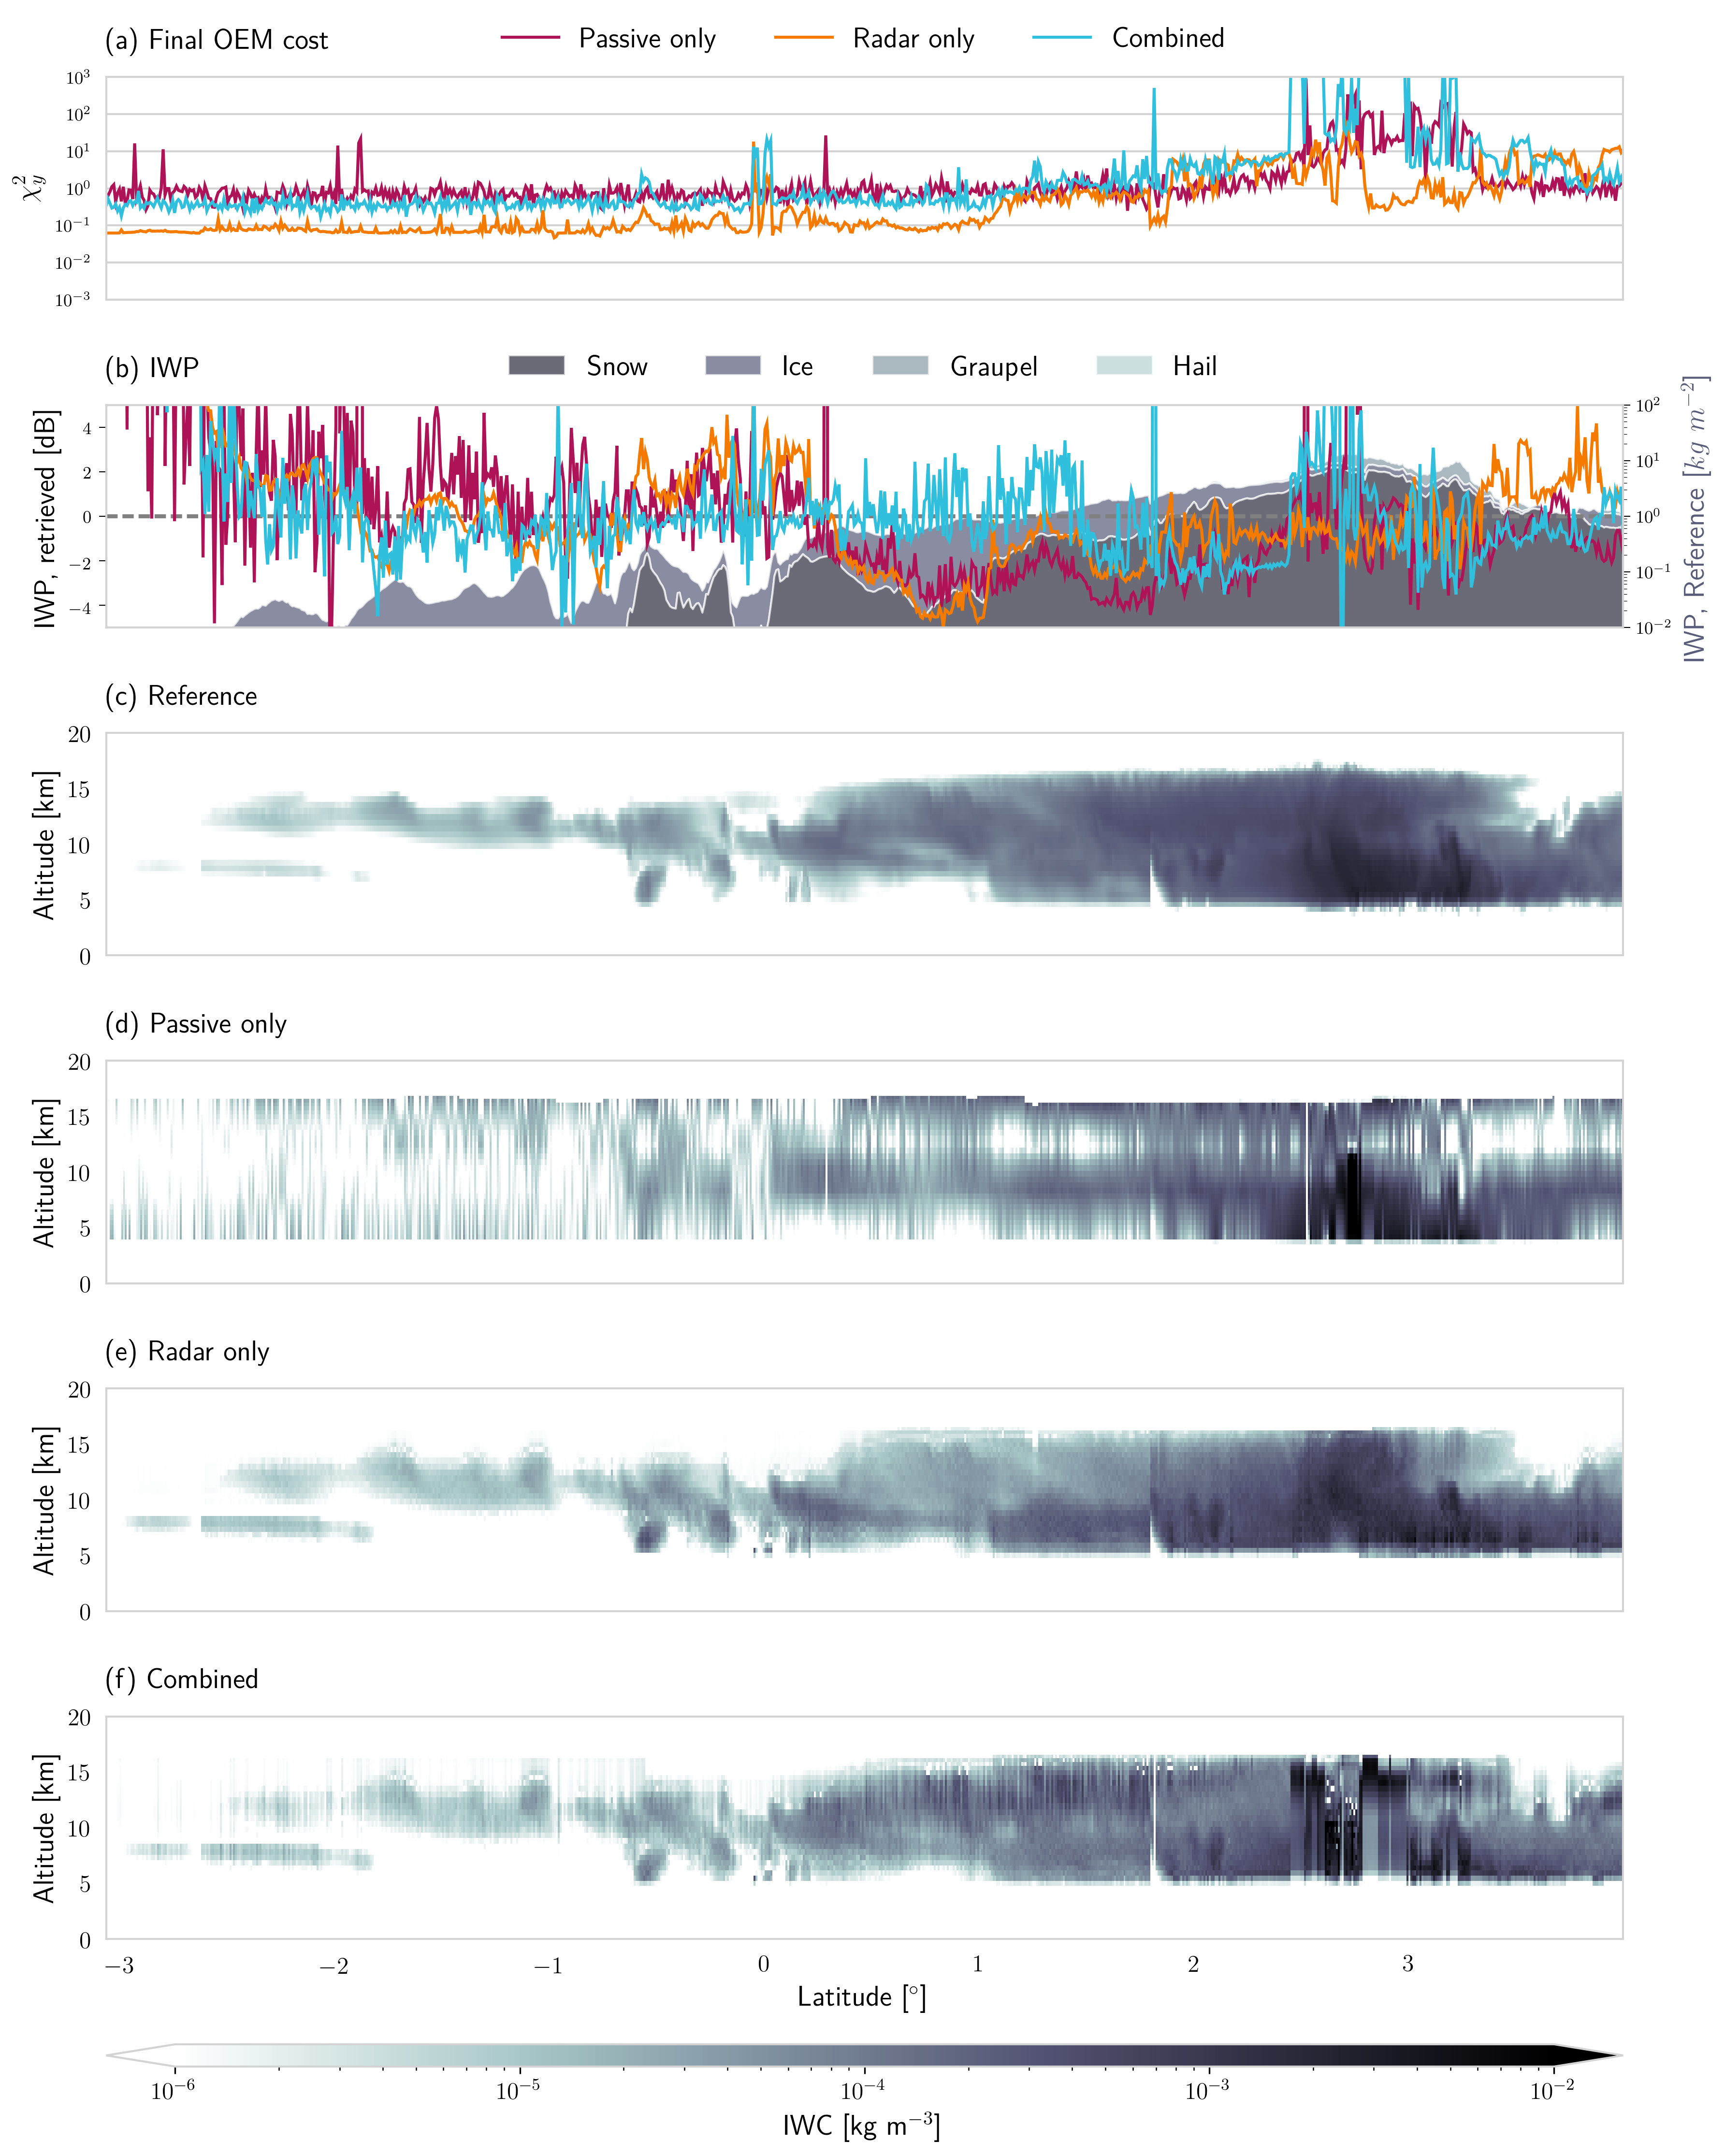
\includegraphics[width = 0.8\textwidth]{../plots/results_a_LargePlateAggregate}
\DIFaddendFL \caption{Results of the ice hydrometeor retrieval for the first test scene.
  Panel (a) displays the value of the $\chi^2_y$ diagnostic normalized by the
  dimension of the measurement space of the corresponding retrieval. Panel (b)
  displays retrieved IWP in dB relative to the reference IWP. \DIFaddbeginFL \DIFaddFL{Absolute
  reference IWP and the contributions from different hydrometeor classes are
  displayed by the filled areas in the background. }\DIFaddendFL Panel (c) shows
  the reference IWC from the model scene. Panel (d), (e) and (f) display the
  retrieval results for the passive-only, radar-only and combined retrieval,
  respectively.}
\label{fig:results_a}
\end{figure}

\DIFdelbegin \DIFdel{To make the }\DIFdelend \DIFaddbegin \DIFadd{For a more quantitative }\DIFaddend assessment of the retrieval performance\DIFdelbegin \DIFdel{more quantitative, the
reference mass concentrations are }\DIFdelend \DIFaddbegin \DIFadd{, retrieved water
content is }\DIFaddend plotted against the \DIFdelbegin \DIFdel{retrieved values }\DIFdelend \DIFaddbegin \DIFadd{reference water content }\DIFaddend in
Fig.~\DIFdelbegin \DIFdel{\ref{fig:results_scatter_a_1} and \ref{fig:results_scatter_a_2}. The plots
show the results for all different retrieval configurations and tested
particle models. Markers in the plots are color-coded according to the
prevailing hydrometeor type (by mass density) in the reference scene in order
to allow assessment of the retrieval performance for the different hydrometeor
types of the GEM model.
}%DIFDELCMD < 

%DIFDELCMD < %%%
\DIFdel{Not surprisingly, the results from the passive-only retrieval exhibit the strongest deviations }\DIFdelend \DIFaddbegin \DIFadd{\ref{fig:results_scatter_a}. In terms of precision, the passive only
retrieval performs worst while both the radar-only and combined retrieval yield
much smaller spread of the retrieved values }\DIFaddend from the diagonal. \DIFdelbegin \DIFdel{Since the passive channels alone contain only limited }\DIFdelend \DIFaddbegin \DIFadd{This is not
surprising considering that the passive observations do not contain sufficient
}\DIFaddend information on the vertical distribution of \DIFdelbegin \DIFdel{ice in the atmosphere,
the retrieval cannot be expected }\DIFdelend \DIFaddbegin \DIFadd{IWC }\DIFaddend to yield accurate results at the
resolution \DIFdelbegin \DIFdel{considered here. Although rather weak, a certain effect of the ice particle
model on the retrieval results can be observed. In particular, the GemCloudIce model
leads to a systematic underestimation of ice mass densities, which are less
pronounced for the other particle models.}%DIFDELCMD < 

%DIFDELCMD < \begin{figure}
%DIFDELCMD < \centering \includegraphics[width = 0.8\textwidth]{figures/fig07}
%DIFDELCMD < %%%
%DIFDELCMD < \caption{%
{%DIFAUXCMD
\DIFdelFL{Reference IWC plotted against retrieved IWC for the tested retrieval
  configurations. Each row shows the retrieval results for the particle shape
  shown in the first panel. The following panels show the retrieval results for
  the passive only (first column), the radar only (second column) and the
  combined retrieval (third column). Markers are colored according to the
  prevailing hydrometeor type at the corresponding grid point in the test
  scene. Due to their sparsity, markers corresponding to graupel are drawn at
  twice the size of the other markers.}}
%DIFAUXCMD
%DIFDELCMD < \label{fig:results_scatter_a_1}
%DIFDELCMD < \end{figure}
%DIFDELCMD < 

%DIFDELCMD < %%%
\DIFdel{The results from the radar-only retrieval are more accurate than the
passive-only retrieval, with almost all retrieval results located fairly close
to the diagonal. The most distinct feature of the radar-only results, however, is the emergence of two clusters that extend along the diagonal but are displaced above respectively below it. The color coding of the markers reveals
that these clusters correspond to
grid points dominated by ice for the cluster
below the diagonal and snow for the cluster located above the diagonal. This
indicates }\DIFdelend \DIFaddbegin \DIFadd{of the model scenes. In terms of overall accuracy, i.e. systematic
deviations from the diagonal, no clear differences between the three
configurations are visible. However, the color-coding with respect to
hydrometeor species, reveals }\DIFaddend that the radar-only retrieval \DIFdelbegin \DIFdel{systematically underestimates mass
densities for cloud ice but overestimates the mass density of snow. The effect
is observed for
all tested particle shapes and thus likely independent of it. In general, the radar-only results exhibit only very weak dependency on the particle model, making the results for different particle shapes virtually
indistinguishable.
}%DIFDELCMD < 

%DIFDELCMD < %%%
\DIFdel{Another feature that stands out in the radar-only resultsis that the retrieval
does not work for graupel. This,
however, can be understood by comparing the
radar reflectivities shown in Fig.~\ref{fig:observations_a} with the cloud
structure displayed in Fig.~\ref{fig:overview}. It becomes apparent that graupel
in this scene is located where the radar signal is fully attenuated. Since there
is no signal to retrieve the mass density from, this explains the bad
performance of the radar-only retrieval for these grid points.
}%DIFDELCMD < 

%DIFDELCMD < %%%
\DIFdel{Similar to the radar-only retrieval, the results of the combined retrieval are
located close to the diagonal. But the clusters observed in the radar-only
results are to large extent merged in the combined results. Moreover, except for
the results obtained with the GemCloudIce particle shape, the two clusters move
in closer }\DIFdelend \DIFaddbegin \DIFadd{is biased for
specific hydrometeor classes. In the combined and even the passive-only results,
this effect is weaker and the clusters are generally moved }\DIFaddend towards the diagonal.
\DIFdelbegin \DIFdel{The combined retrieval thus improves the IWC
retrieval for the specific hydrometeor species in the scene.
}%DIFDELCMD < 

%DIFDELCMD < %%%
\DIFdel{Nonetheless, the results for the GemCloudIce particle stand out in the results.
Even though the systematic deviations observed in the radar-only retrieval are
reduced for most particle shapes, for this specific shape they are instead
increased. The retrieval error is particularly large for snow, which is strongly
underestimated for reference mass concentrations around $10^{-4} \ \unit{kg\ m^{-3}}$}\DIFdelend \DIFaddbegin \DIFadd{For graupel, all retrievals perform badly but this likely due to it being
present only in the core of the convective system where the signals from all
sensors can be expected to be saturated}\DIFaddend .

\DIFdelbegin %DIFDELCMD < \begin{figure}
%DIFDELCMD < \centering
%DIFDELCMD < \includegraphics[width = 0.8\textwidth]{figures/fig08}
%DIFDELCMD < %%%
%DIFDELCMD < \caption{%
{%DIFAUXCMD
\DIFdelFL{Same as Fig.~\ref{fig:results_scatter_a_1} but for the remaining particle
  shapes.}}
%DIFAUXCMD
%DIFDELCMD < \label{fig:results_scatter_a_2}
%DIFDELCMD < \end{figure}
%DIFDELCMD < 

%DIFDELCMD < %%%
\DIFdel{The results for the second test scene obtained using the LargePlateAggregate
particle model are shown in Fig.~\ref{fig:results_b}. As mentioned above, the
results are qualitatively very similar to those of the first scene. Also here,
the final OEM cost, shown in Panel~(a), displays a region of increased cost for
}\DIFdelend \DIFaddbegin \DIFadd{Comparing the results for different particle models, a clear dependency is
evident in }\DIFaddend the passive-only and \DIFdelbegin \DIFdel{combined retrievals. This is again a region of very dense
cloud which consists of graupel and snow. Also similar to the first scene, the passive only retrieval does not reproduce the structure of the cloud well.
Although the cloud top is placed at the right position, neither the vertical
structure of the cloud nor its base are resolved. The radar-only retrieval
resolves the vertical structure of the cloud well, but overestimates the ice
mass density in the scene. The combined retrieval also resolves the vertical
structure of the cloud well and corrects the overestimation observed in the
radar-only results to some extent.
}%DIFDELCMD < 

%DIFDELCMD < \begin{figure}
%DIFDELCMD < \centering
%DIFDELCMD < \includegraphics[width = 0.8\textwidth]{figures/fig09}
%DIFDELCMD < %%%
%DIFDELCMD < \caption{%
{%DIFAUXCMD
\DIFdelFL{Results of the ice hydrometeor retrieval for the second test scene.
  Panel (a) displays the value of the $\chi^2_y$ diagnostic normalized by the
  dimension of the measurement space of the corresponding retrieval. Panel (b)
  shows retrieved IWP in dB relative to the reference IWP. Panel (c) displays
  the reference mass concentrations from the model scene. Panel (d), (e) and (f)
  display the retrieval results for the passive-only, radar-only and combined
  retrieval, respectively.}}
%DIFAUXCMD
%DIFDELCMD < \label{fig:results_b}
%DIFDELCMD < \end{figure}
%DIFDELCMD < 

%DIFDELCMD < %%%
\DIFdel{Scatter plots for the retrieval results from the second scene are shown in
Fig.~\ref{fig:results_scatter_b_1}. Except for the lack of cloud ice in the scene, }\DIFdelend the \DIFdelbegin \DIFdel{results are similar to what has been observed in the first scene: The
radar-only retrieval overestimates the mass density of snow in the scene. This
effect is corrected by the combined retrieval for most of the tested particle
shapes. The exception is the GemCloudIce particle for which the retrieval of
snow particle deteriorates quite drastically}\DIFdelend \DIFaddbegin \DIFadd{combined results whereas the radar-only
retrieval is affected the least. For both the combined and passive-only
retrieval the effect is consistent across the methods, with the GEM Cloud Ice
and Large Column Aggregate yielding the largest deviations and the Large Plate
Aggregate yielding the most accurate results}\DIFaddend .

\DIFdelbegin %DIFDELCMD < \begin{figure}[!h]
%DIFDELCMD < %%%
\DIFdelendFL \DIFaddbeginFL \begin{figure}
\DIFaddendFL \centering \DIFdelbeginFL %DIFDELCMD < \includegraphics[width = 0.8\textwidth]{figures/fig10}
%DIFDELCMD < %%%
\DIFdelendFL \DIFaddbeginFL 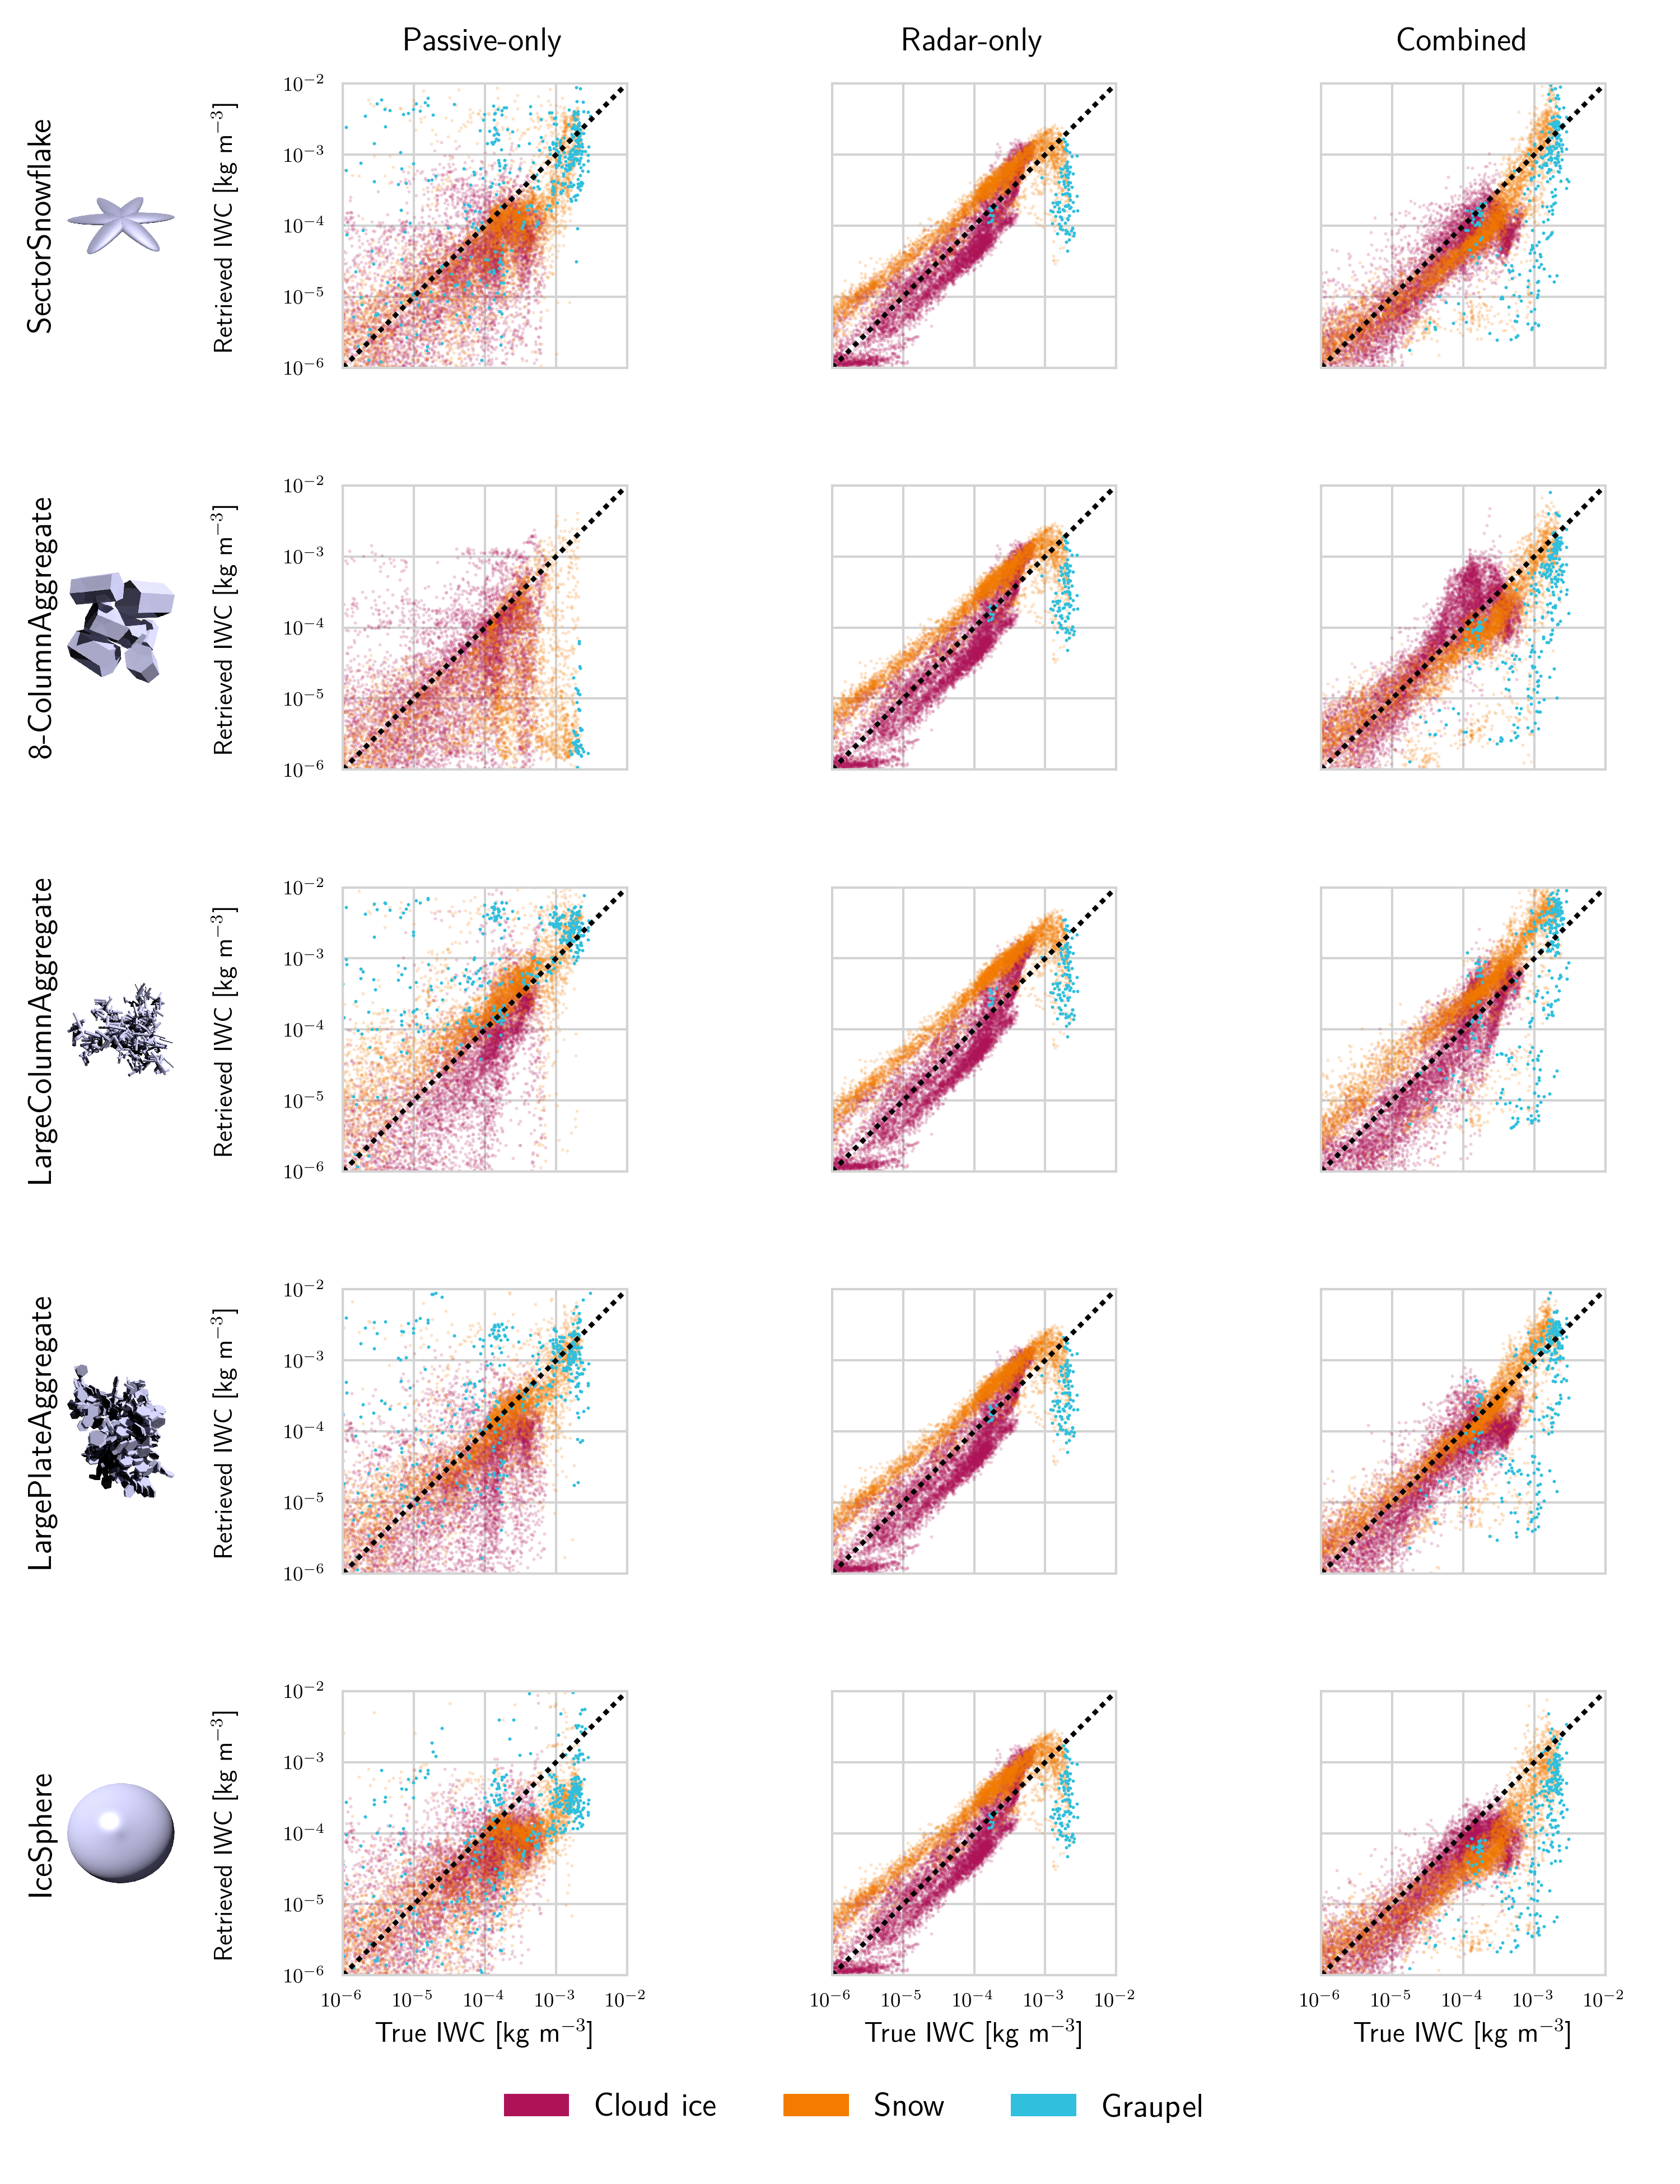
\includegraphics[width = 0.75\textwidth]{../plots/results_scatter_a}
\DIFaddendFL \caption{\DIFdelbeginFL \DIFdelFL{Scatter plots of the }\DIFdelendFL \DIFaddbeginFL \DIFaddFL{Retrieved IWC plotted against }\DIFaddendFL reference \DIFdelbeginFL \DIFdelFL{and retrieved ice mass densities }\DIFdelendFL \DIFaddbeginFL \DIFaddFL{IWC }\DIFaddendFL for the \DIFdelbeginFL \DIFdelFL{second test scene}\DIFdelendFL \DIFaddbeginFL \DIFaddFL{tested retrieval
  configurations}\DIFaddendFL . \DIFdelbeginFL \DIFdelFL{The rows show }\DIFdelendFL \DIFaddbeginFL \DIFaddFL{Each row shows }\DIFaddendFL the retrieval results for \DIFdelbeginFL \DIFdelFL{a given
  assumed ice particle model. The first column of each row displays a rendering
  of }\DIFdelendFL the particle \DIFdelbeginFL \DIFdelFL{model}\DIFdelendFL \DIFaddbeginFL \DIFaddFL{shape
  shown in the first panel}\DIFaddendFL . The following \DIFdelbeginFL \DIFdelFL{rows display }\DIFdelendFL \DIFaddbeginFL \DIFaddFL{panels show }\DIFaddendFL the \DIFaddbeginFL \DIFaddFL{retrieval }\DIFaddendFL results for
  the \DIFdelbeginFL \DIFdelFL{passive-only}\DIFdelendFL \DIFaddbeginFL \DIFaddFL{passive only (first column)}\DIFaddendFL , the \DIFdelbeginFL \DIFdelFL{radar-only }\DIFdelendFL \DIFaddbeginFL \DIFaddFL{radar only (second column) }\DIFaddendFL and the
  combined retrieval \DIFaddbeginFL \DIFaddFL{(third column). Markers are colored according to the
  prevailing hydrometeor type at the corresponding grid point in the test
  scene. Due to their sparsity, markers corresponding to graupel are drawn at
  twice the size of the other markers}\DIFaddendFL .}
\DIFdelbeginFL %DIFDELCMD < \label{fig:results_scatter_b_1}
%DIFDELCMD < %%%
\DIFdelendFL \DIFaddbeginFL \label{fig:results_scatter_a}
\DIFaddendFL \end{figure}



To summarize retrieval performance for all tested retrieval methods and particle
shapes, the \DIFaddbegin \DIFadd{distributions of the }\DIFaddend logarithmic error
\begin{align}
  \text{E}_{\text{log}_{10}} &= \log_\text{10} \left
  (\frac{x_\text{retrieved}}{x_\text{reference}} \right )
\end{align}
for the retrieved IWC and IWP are displayed in Fig.~\ref{fig:boxes}. \DIFdelbegin \DIFdel{The
logarithmic error in the IWC retrieval }\DIFdelend \DIFaddbegin \DIFadd{In this
also results from the 1M version of the radar-only retrieval are presented since
it can actually perform better than the two-moment version.
}

\DIFadd{For IWC, the error }\DIFaddend has been computed \DIFdelbegin \DIFdel{only for }\DIFdelend \DIFaddbegin \DIFadd{considering only }\DIFaddend grid points where either
reference or retrieved IWC is larger than $10^{-6}\ \unit{kg\ m^{-3}}$. \DIFdelbegin \DIFdel{Considering first the results of the IWC
retrieval, shown in Panel~(a) and (b), the plots }\DIFdelend \DIFaddbegin \DIFadd{The
results }\DIFaddend confirm the findings \DIFdelbegin \DIFdel{from }\DIFdelend \DIFaddbegin \DIFadd{of }\DIFaddend the analysis above: The combined retrieval
\DIFdelbegin \DIFdel{generally }\DIFdelend yields the smallest retrieval errors \DIFaddbegin \DIFadd{for suitable choices of the particle model}\DIFaddend .
Although the \DIFdelbegin \DIFdel{spread of the retrieval errors }\DIFdelend \DIFaddbegin \DIFadd{two-moment radar-only retrieval performs similar to the combined
retrieval in terms of precision, it yields significant systematic errors for the
second scene. The reason for this can be understood considering the cloud
composition displayed in Fig.~\ref{fig:overview}. The clouds in the second test
scene consist to largest part of snow. The bias }\DIFaddend of the radar-only retrieval \DIFdelbegin \DIFdel{is lower in
}\DIFdelend \DIFaddbegin \DIFadd{with
respect to this specific hydrometeor species, which can be observed in
Fig.~\ref{fig:results_scatter_a} and also Fig.~\ref{fig:results_scatter_b},
leads to the large observed systematic errors for the second scene. The
single-moment radar-only retrieval does not produce the same large systematic
errors for }\DIFaddend the second scene, \DIFdelbegin \DIFdel{the combined retrieval yields smaller systematic
errors }\DIFdelend \DIFaddbegin \DIFadd{but instead produces systematic errors for the
first scene. The passive-only retrieval yields the largest errors in terms of
retrieved IWC due its low vertical resolution}\DIFaddend .

\DIFdelbegin \DIFdel{Compared in }\DIFdelend \DIFaddbegin \DIFadd{In }\DIFaddend terms of IWP, however, the \DIFdelbegin \DIFdel{results are different. Especially }\DIFdelend \DIFaddbegin \DIFadd{errors of }\DIFaddend the passive-only retrieval \DIFdelbegin \DIFdel{yields much lower errors for the retrieved IWP, }\DIFdelend \DIFaddbegin \DIFadd{decrease
significantly }\DIFaddend making the results comparable \DIFdelbegin \DIFdel{if not better than }\DIFdelend \DIFaddbegin \DIFadd{to }\DIFaddend those of the other methods. For
the radar-only and combined retrievals\DIFaddbegin \DIFadd{, }\DIFaddend the precision is generally increased but
\DIFaddbegin \DIFadd{the }\DIFaddend systematic deviations observed \DIFdelbegin \DIFdel{in the }\DIFdelend \DIFaddbegin \DIFadd{for }\DIFaddend IWC persist. This leads, particularly for
the second test scene, to significant systematic errors in the
\DIFdelbegin \DIFdel{radar-only-retrieved IWP }\DIFdelend \DIFaddbegin \DIFadd{IWP retrieved by the two-moment radar-only retrieval}\DIFaddend .

\DIFdelbegin \DIFdel{In addition to this, the passive-only and the combined retrieval exhibit }\DIFdelend \DIFaddbegin \DIFadd{Also in these results, }\DIFaddend a strong dependence \DIFdelbegin \DIFdel{of the retrieval error }\DIFdelend on the applied particle model \DIFdelbegin \DIFdel{.
Especially the GemCloudIce and GemSnow particle models yield large retrieval
errors for IWC and IWP. The other three particle models, however, consistently
yield smaller retrievalthan the GemCloudIce and GemSnow models}\DIFdelend \DIFaddbegin \DIFadd{is
observed for the passive-only and combined retrievals. The errors are
particularly large for the GEM Cloud Ice and the Large Column Aggregate. For the
radar-only retrieval, the particle shape has less impact on the retrieval
performance and does not effect the large systematic errors observed for the
second test scene}\DIFaddend .

\begin{figure}[!h]
\centering \DIFdelbeginFL %DIFDELCMD < \includegraphics[width = 0.8\textwidth]{figures/fig11}
%DIFDELCMD < %%%
\DIFdelendFL \DIFaddbeginFL 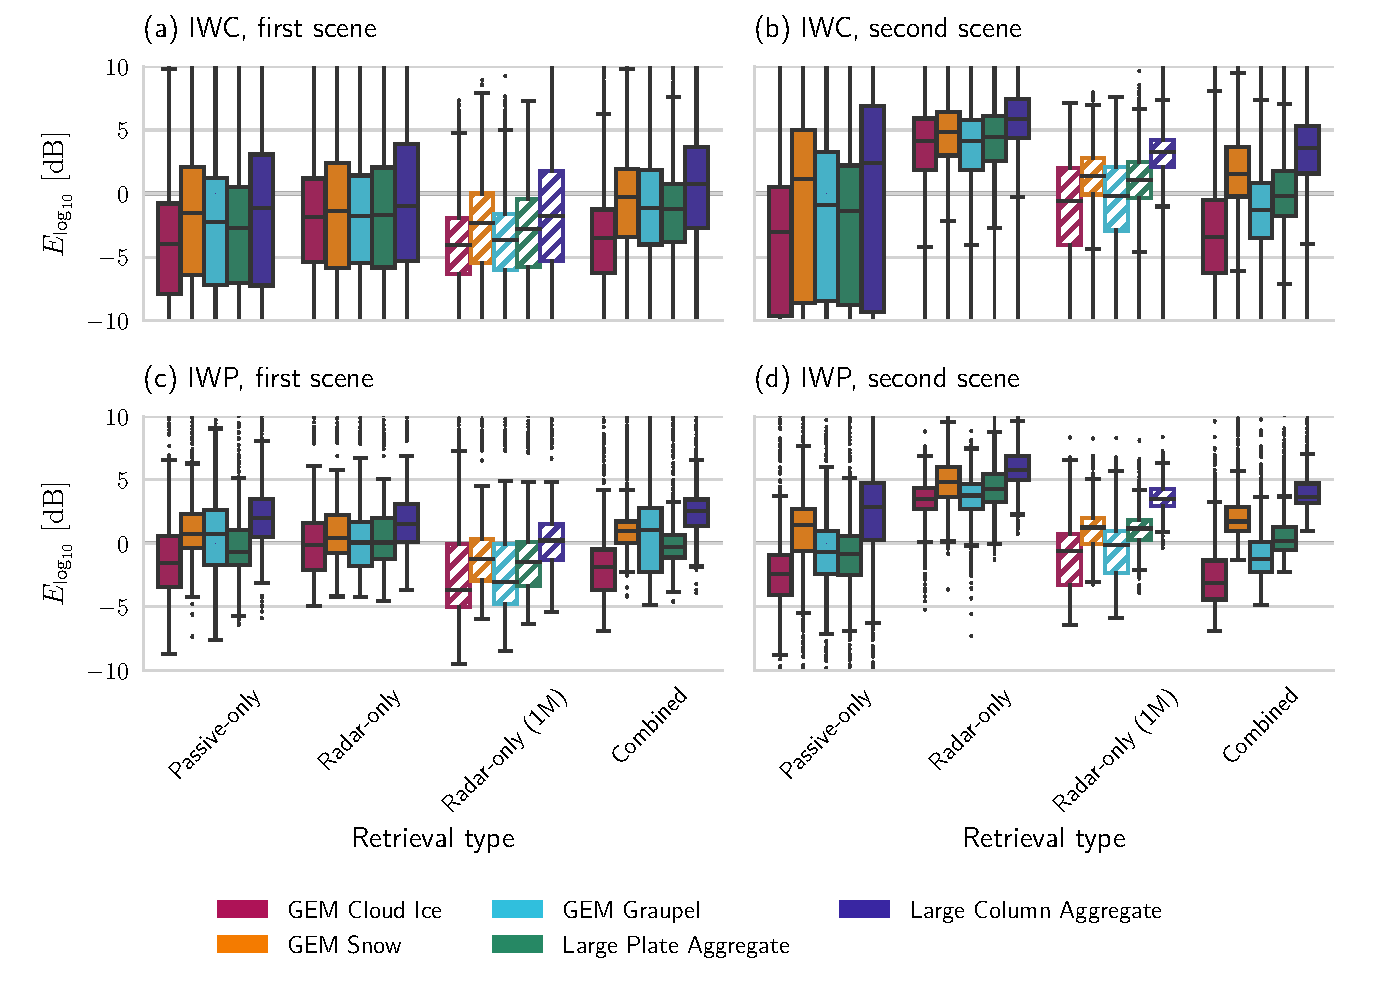
\includegraphics[width = 0.8\textwidth]{../plots/results_box}
\DIFaddendFL \caption{Distributions of the logarithmic retrieval error in IWC and IWP for all
  tested retrieval methods and particle shapes displayed as box plots. Colored
  boxes display the interquartile range (IQR) while whiskers show full range of
  all points not considered outliers. Points whose distance to the IQR is larger
  than 1.5 times the width of the IQR are considered outliers and drawn as
  markers. \DIFaddbeginFL \DIFaddFL{Two results are shown for the radar-only retrieval, one for the
  standard version retrieving both PSD moments (solid boxes) and one for a
  single-moment (1M) version (diagonal hatches).}\DIFaddendFL }
\label{fig:boxes}
\end{figure}

\subsubsection{Particle number densities}

Particle number densities of frozen hydrometeors have been derived from the
retrieved $N_0^*$ and $D_m$ parameters by computing the zeroth moment of the
corresponding PSD. The resulting particle number density fields are displayed
together with the reference field in Fig.~\ref{fig:results_nd_a}. To simplify
the comparison\DIFaddbegin \DIFadd{, }\DIFaddend number densities are displayed only where the corresponding
reference or retrieved IWC is larger than $10^{-6}\ \unit{kg\ m^{-3}}$.

Comparing the passive-only and the radar-only retrieval to the reference \DIFdelbegin \DIFdel{field
}\DIFdelend \DIFaddbegin \DIFadd{fields
}\DIFaddend shows that both methods have little to no skill in predicting number density
concentrations. Although the passive-only retrieval partly captures the gradient
between very high concentrations at the top of the cloud and the low
concentrations at the bottom, it is not at all resolved in the radar-only
retrieval.
\DIFdelbegin \DIFdel{The combined retrieval , however, }\DIFdelend \DIFaddbegin 

\DIFadd{In contrast to this, the combined retrieval }\DIFaddend manages to reproduce this gradient
in \DIFdelbegin \DIFdel{some }\DIFdelend \DIFaddbegin \DIFadd{most }\DIFaddend parts of the scene. \DIFdelbegin \DIFdel{Although its exact structure is not fully
reproduced, this clearly shows sensitivity of the retrievals to particle number
concentrations.
}%DIFDELCMD < 

%DIFDELCMD < %%%
\DIFdel{The combined retrieval shows the strongest deviations }\DIFdelend \DIFaddbegin \DIFadd{The strongest deviations of the combined results
}\DIFaddend from the reference field \DIFaddbegin \DIFadd{are observed }\DIFaddend between $2$ and $3\unit{^\circ}$ latitude.
Here, the results strongly underestimate the true number concentrations.
Comparison with the cloud composition displayed in Panel (a) of
Fig.~\ref{fig:overview} shows that this region contains large amounts of both
cloud ice and snow. \DIFdelbegin \DIFdel{Since the }\DIFdelend \DIFaddbegin \DIFadd{The }\DIFaddend retrieval uses only a single hydrometeor species to
represent ice in the atmosphere \DIFdelbegin \DIFdel{it is }\DIFdelend \DIFaddbegin \DIFadd{and is therefore }\DIFaddend not able to represent such
heterogeneous conditions. Since snow will have \DIFdelbegin \DIFdel{the
}\DIFdelend stronger impact on the
observations, the retrieval in these regions \DIFdelbegin \DIFdel{tends to predict }\DIFdelend \DIFaddbegin \DIFadd{will likely tend to represent }\DIFaddend snow
rather than ice, which leads to the low retrieved number densities.

\DIFdelbegin \DIFdel{To further investigate this, }\DIFdelend \DIFaddbegin \begin{figure}
\centering
\includegraphics[width = 0.7\textwidth]{../plots/results_nd_a_LargePlateAggregate}
\caption{\DIFaddFL{Reference and retrieved particle number concentrations of frozen
  hydrometeors for the first test scene obtained with the LargePlateAggregate
  particle model. Panel (a) displays the reference mass concentrations from the
  model scene. Panel (b), (c) and (d) display the retrieval results for the
  passive-only, radar-only and combined retrieval. Only values for which the
  corresponding reference or retrieved IWC was larger than
  $10^{-6}\ \unit{kg\ m^{-3}}$ are shown here.}}
\label{fig:results_nd_a}
\end{figure}

\DIFaddend Fig.~\ref{fig:results_nd_scatter_a} displays scatter plots of the reference and
retrieved number density concentrations for all three methods and two particle
models from the first test scene. Markers in the plot are color coded according
to their homogeneity in the reference scene, here defined as the ratio of the
maximum \DIFdelbegin \DIFdel{mass density }\DIFdelend \DIFaddbegin \DIFadd{water content }\DIFaddend of any of the frozen hydrometeor species and total IWC.
\DIFdelbegin %DIFDELCMD < 

%DIFDELCMD < \begin{figure}
%DIFDELCMD < \centering
%DIFDELCMD < \includegraphics[width = 0.7\textwidth]{figures/fig12}
%DIFDELCMD < %%%
%DIFDELCMD < \caption{%
{%DIFAUXCMD
\DIFdelFL{Reference and retrieved particle number concentrations of frozen
  hydrometeors for the first test scene obtained with the LargePlateAggregate
  particle model. Panel (a) displays the reference mass concentrations from the
  model scene. Panel (b), (c) and (d) display the retrieval results for the
  passive-only, radar-only and combined retrieval. Only values for which the corresponding
  reference or retrieved IWC was larger than  $10^{-6}\ \unit{kg\ m^{-3}}$ are shown here.}}
%DIFAUXCMD
%DIFDELCMD < \label{fig:results_nd_a}
%DIFDELCMD < \end{figure}
%DIFDELCMD < 

%DIFDELCMD < %%%
\DIFdelend These results confirm that the passive-only retrieval possesses \DIFdelbegin \DIFdel{certain
}\DIFdelend \DIFaddbegin \DIFadd{some }\DIFaddend sensitivity
to the particle number density since the cluster at low \DIFdelbegin \DIFdel{reference
number
densities }\DIFdelend \DIFaddbegin \DIFadd{particle number
concentrations }\DIFaddend corresponding to snow is placed correctly on the diagonal\DIFaddbegin \DIFadd{, which
is not the case for the radar-only retrieval}\DIFaddend . The radar-only retrieval does not
exhibit any retrieval skill, hardly reproducing any of the variation of the
\DIFdelbegin \DIFdel{references }\DIFdelend \DIFaddbegin \DIFadd{reference }\DIFaddend values. Contrary to this, the combined retrieval moves both clusters\DIFaddbegin \DIFadd{,
the one corresponding to snow and the one at high number concentrations
corresponding to cloud ice, }\DIFaddend towards the diagonal\DIFdelbegin \DIFdel{, indicating }\DIFdelend \DIFaddbegin \DIFadd{. This indicates }\DIFaddend that it is
capable of distinguishing the microphysical properties of cloud ice and snow.
Furthermore, the color coding shows that the strongest deviations between
retrieved and reference number densities occur for grid points where the cloud
composition is heterogeneous. 
\DIFdelbegin \DIFdel{Even for the combined retrieval, however, the
accuracy of a single retrieval value remains fairly low.
}\DIFdelend 

The \DIFaddbegin \DIFadd{general }\DIFaddend effect of particle shape on the retrieval results is \DIFdelbegin \DIFdel{somewhat }\DIFdelend similar to what
has been observed for IWC\DIFaddbegin \DIFadd{, which is why only results for two particle shapes are
shown}\DIFaddend . For the passive-only and combined retrieval, the \DIFdelbegin \DIFdel{GemCloudIce model again yields }\DIFdelend \DIFaddbegin \DIFadd{GEM Cloud Ice and Large
Column Aggregate models yield }\DIFaddend the worst retrieval results, \DIFdelbegin \DIFdel{leading to a general
underestimation of the true particle number density}\DIFdelend \DIFaddbegin \DIFadd{while the Large Plate
Aggregate performs best}\DIFaddend . For the radar-only retrieval no noticeable differences
are observed between different particle models.
\DIFdelbegin \DIFdel{Only the results for the GemCloudIce and LargePlateAggregate particle
models are shown here since the results for the other particles are mostly similar
to those obtained with the LargePlateAggregate model.
}\DIFdelend 

\begin{figure}
\centering
\includegraphics[width = 0.7\textwidth]{figures/fig13}
\caption{Scatter plots of the retrieved particle number densities at grid points
  with reference \DIFdelbeginFL \DIFdelFL{mass density }\DIFdelendFL \DIFaddbeginFL \DIFaddFL{IWC }\DIFaddendFL larger than $10^{-5}\ \unit{kg\ m^{-3}}$. Rows show
  the results for the different particle models used in the retrieval while
  \DIFdelbeginFL \DIFdelFL{column }\DIFdelendFL \DIFaddbeginFL \DIFaddFL{columns }\DIFaddendFL display  \DIFdelbeginFL \DIFdelFL{the }\DIFdelendFL results for  \DIFdelbeginFL \DIFdelFL{the }\DIFdelendFL different retrieval methods. The marker
  color encodes the homogeneity of the corresponding ice mass, which is computed
  as the ratio of the maximum \DIFdelbeginFL \DIFdelFL{mass density }\DIFdelendFL \DIFaddbeginFL \DIFaddFL{water content }\DIFaddendFL of any of the frozen hydrometeor
  species and total IWC.}
\label{fig:results_nd_scatter_a}
\end{figure}

\subsubsection{Information content}

\DIFdelbegin \DIFdel{The retrieval results presented above show that the combined observations allow
a more accurate retrieval of both mass and particle number density. This
confirms the experimental results from Sec.~\ref{sec:simple_cloud}, that active
and passive observations provide complementary information on the microphysics
of ice particles. The }\DIFdelend \DIFaddbegin \DIFadd{To quantify the }\DIFaddend information content of the \DIFdelbegin \DIFdel{retrievals can be assessed more
quantitatively using the averaging kernel matrix. The trace of the AVK, commonly
referred to as the number of }\DIFdelend \DIFaddbegin \DIFadd{single-instrument and the combined
observations the }\DIFaddend degrees of freedom for signal (DFS) \DIFdelbegin \DIFdel{, quantifies the
number of independent pieces of information contained in the observations.
}%DIFDELCMD < 

%DIFDELCMD < %%%
\DIFdel{The distributions of the degrees of freedom of }\DIFdelend \DIFaddbegin \DIFadd{have been computed
following the common approach \mbox{%DIFAUXCMD
\citep{rodgers00, mahfouf15, grutzun18} }\hspace{0pt}%DIFAUXCMD
and are
displayed for }\DIFaddend each retrieved profile in the test scenes \DIFdelbegin \DIFdel{are displayed }\DIFdelend in Fig.~\DIFdelbegin \DIFdel{\ref{fig:dofs}.
Not-surprisingly, the combined
observations exhibit the highest }\DIFdelend \DIFaddbegin \DIFadd{\ref{fig:dfs}.
}

\DIFadd{With respect to ice, the passive-only retrieval yields the lowest }\DIFaddend information
content. \DIFdelbegin \DIFdel{Nevertheless, comparison
with the DFS values of the active- and passive-only retrieval shows that the observations contain a certain degree of redundancy leading to a lower combined
DFS value than the direct sum of }\DIFdelend \DIFaddbegin \DIFadd{For the radar-only retrieval }\DIFaddend the \DIFdelbegin \DIFdel{two. }\DIFdelend \DIFaddbegin \DIFadd{information content is significantly
higher, on the order of 20 degrees of freedom, but the major part of it is
attributed to the $D_m$ parameter. For the combined retrieval, the total
information content on ice hydrometeors is generally increased in regions where
the passive observations provides information on frozen hydrometeors. In
addition to that, a clear shift of information content from $D_m$ to $N_0^*$ can
be observed over both scenes.
}\DIFaddend 

\DIFdelbegin \DIFdel{The grouping into retrieval quantities furthermore reveals that the largest
increase in the information content comes from water vapor, which is not
retrieved in the radar-only retrieval. Although small, a significant increase in
information content is observed for both scenes}\DIFdelend \DIFaddbegin \DIFadd{The information content for rain is much smaller but in relative terms the
general behavior is the same as for ice. For RH, no difference is observed }\DIFaddend for
the \DIFdelbegin \DIFdel{$N_0^*$ parameter for icehydrometeors. Interestingly, this increase is observed even though the
}\DIFdelend information content \DIFdelbegin \DIFdel{in }\DIFdelend \DIFaddbegin \DIFadd{provided by }\DIFaddend the passive-only \DIFdelbegin \DIFdel{observations for $N_0^*$ is close to
zero.
For the $D_m$ parameter, a small decrease is observed with respect to the
radar-only retrieval for both scenes. Since the calculation of the AVK involves
the forward model Jacobian, this effect must be related to the non-linearity of the forward model}\DIFdelend \DIFaddbegin \DIFadd{and combined retrievals.
For LCWC, a slight increase in the information content of the combined
observations compared to the passive-only observations, but the information
content remains limited to a few degrees of freedom}\DIFaddend .

\begin{figure}
\centering
\DIFdelbeginFL %DIFDELCMD < \includegraphics[width = 0.7\textwidth]{figures/fig14}
%DIFDELCMD < %%%
\DIFdelendFL \DIFaddbeginFL 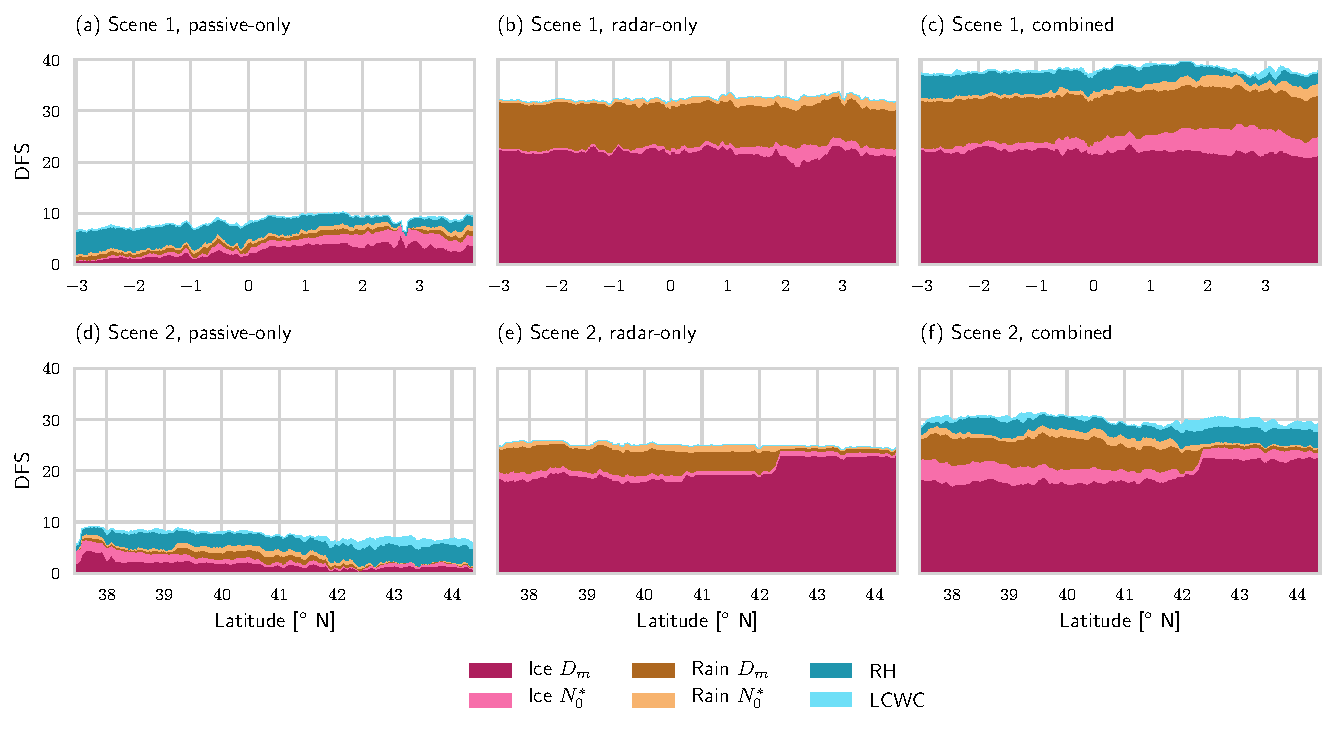
\includegraphics[width = 1.0\textwidth]{../plots/dfs}
\DIFaddendFL \caption{\DIFdelbeginFL \DIFdelFL{Distributions }\DIFdelendFL \DIFaddbeginFL \DIFaddFL{Degrees }\DIFaddendFL of \DIFaddbeginFL \DIFaddFL{freedom for signal for all retrieval configurations and both
  test scenes obtained with the Large Plate Aggregate model. The colored areas
  in each plot represent the contribution to the cumulative }\DIFaddendFL degrees of freedom
  \DIFdelbeginFL \DIFdelFL{of signal displayed as bar plots
  grouped by }\DIFdelendFL \DIFaddbeginFL \DIFaddFL{from each }\DIFaddendFL retrieval quantity\DIFdelbeginFL \DIFdelFL{and method}\DIFdelendFL . Results for the first \DIFaddbeginFL \DIFaddFL{and second }\DIFaddendFL test scene
  are displayed in \DIFdelbeginFL \DIFdelFL{Panel (a) and for }\DIFdelendFL the \DIFaddbeginFL \DIFaddFL{first and }\DIFaddendFL second \DIFdelbeginFL \DIFdelFL{test scene in Panel (b)}\DIFdelendFL \DIFaddbeginFL \DIFaddFL{row, respectively}\DIFaddendFL . \DIFdelbeginFL \DIFdelFL{Markers on
  }\DIFdelendFL \DIFaddbeginFL \DIFaddFL{The first, second
  and third panel in each row show }\DIFaddendFL the \DIFdelbeginFL \DIFdelFL{top of bars mark }\DIFdelendFL \DIFaddbeginFL \DIFaddFL{results for }\DIFaddendFL the \DIFdelbeginFL \DIFdelFL{extent of one standard deviation around }\DIFdelendFL \DIFaddbeginFL \DIFaddFL{passive-only, radar-only
  and }\DIFaddendFL the \DIFdelbeginFL \DIFdelFL{mean of
  each distribution}\DIFdelendFL \DIFaddbeginFL \DIFaddFL{combined retrieval}\DIFaddendFL .}
\DIFdelbeginFL %DIFDELCMD < \label{fig:dofs}
%DIFDELCMD < %%%
\DIFdelendFL \DIFaddbeginFL \label{fig:dfs}
\DIFaddendFL \end{figure}

\subsubsection{Impact of assumed ice particle shape}

\DIFdelbegin \DIFdel{To further investigate the effect }\DIFdelend \DIFaddbegin \DIFadd{The impact }\DIFaddend of the assumed ice particle shape on the retrieval results \DIFdelbegin \DIFdel{, the mass density relations for the tested particle models }\DIFdelend \DIFaddbegin \DIFadd{raises the
question raised whether it also affects the quality of the fit to the
observations. To investigate this, the residuals for the radar observations and
three ICI channels }\DIFaddend are displayed in \DIFdelbegin \DIFdel{Panel~(a) of }\DIFdelend Fig.~\DIFdelbegin \DIFdel{\ref{fig:costs}. As can be seen from this plot,
the GemCloudIce particle clearly stands out due to its large mass. Except for
the fact that the GemSnow particle does not reach down to small particle sizes,
the remaining particle models have quite similar in mass-size relations. The
extreme density of the GemCloudIce particle model for large particle sizes likely
explains the bad performance observedin the results presented above. Similarly,
the bad performance of the GemSnow model in terms of retrieved IWC and IWP is likely
due to it not covering small particle sizes.
}%DIFDELCMD < 

%DIFDELCMD < %%%
\DIFdel{Also displayed in Fig.~\ref{fig:costs} (panel (b) and (c)) are the $\chi^2_y$
values of the combined retrieval obtained for the tested particle models }\DIFdelend \DIFaddbegin \DIFadd{\ref{fig:misfit}. Each test scene
contains a region where the retrieval does not fit the observations well and
where substantial deviations between the fitted and true observations are
observed}\DIFaddend . \DIFdelbegin \DIFdel{Since
the particle shape has considerable effect on sub-millimeter observations \mbox{%DIFAUXCMD
\citep{ekelund19}}\hspace{0pt}%DIFAUXCMD
, one could hope that the retrieval results can be used to infer the prevailing ice particle type based on the how well the
retrieval can
fit the observations . Unfortunately, such clear conclusions cannot be drawn from
the results. In the first test scene, the best fit is obtained by the GemSnow,
GemCloudIce and the LargePlateAggregate particlemodels, although the GemSnow
and GemCloudIce models quite clearly yield the worst retrieval performance. For
the second scene, similar results are
observed . Here, the GemSnow particle
consistently gives the lowest $\chi^2_y$ value but comparison with
Fig.~\ref{fig:boxes} clearly shows that it does not yield the best retrieval
performance}\DIFdelend \DIFaddbegin \DIFadd{It is also in these regions, where the fits obtained with different
particle models differ. These are both regions where the cloud is very thick and
both the radar and passive observations are likely saturated. Since these are
difficult regions for the retrieval it remains unclear whether these differences
can be related directly to the assumed particle shape. In contrast to this, the
retrieval fits the observations well in the remaining parts of the scene. The
exception is the GEM Graupel particle, for which quite significant misfits are
observed between $0$ and $1^{\circ}$ latitude}\DIFaddend .


\begin{figure}[!h]
\centering
\DIFdelbeginFL %DIFDELCMD < \includegraphics[width = 0.8\textwidth]{figures/fig15}
%DIFDELCMD < %%%
\DIFdelendFL \DIFaddbeginFL 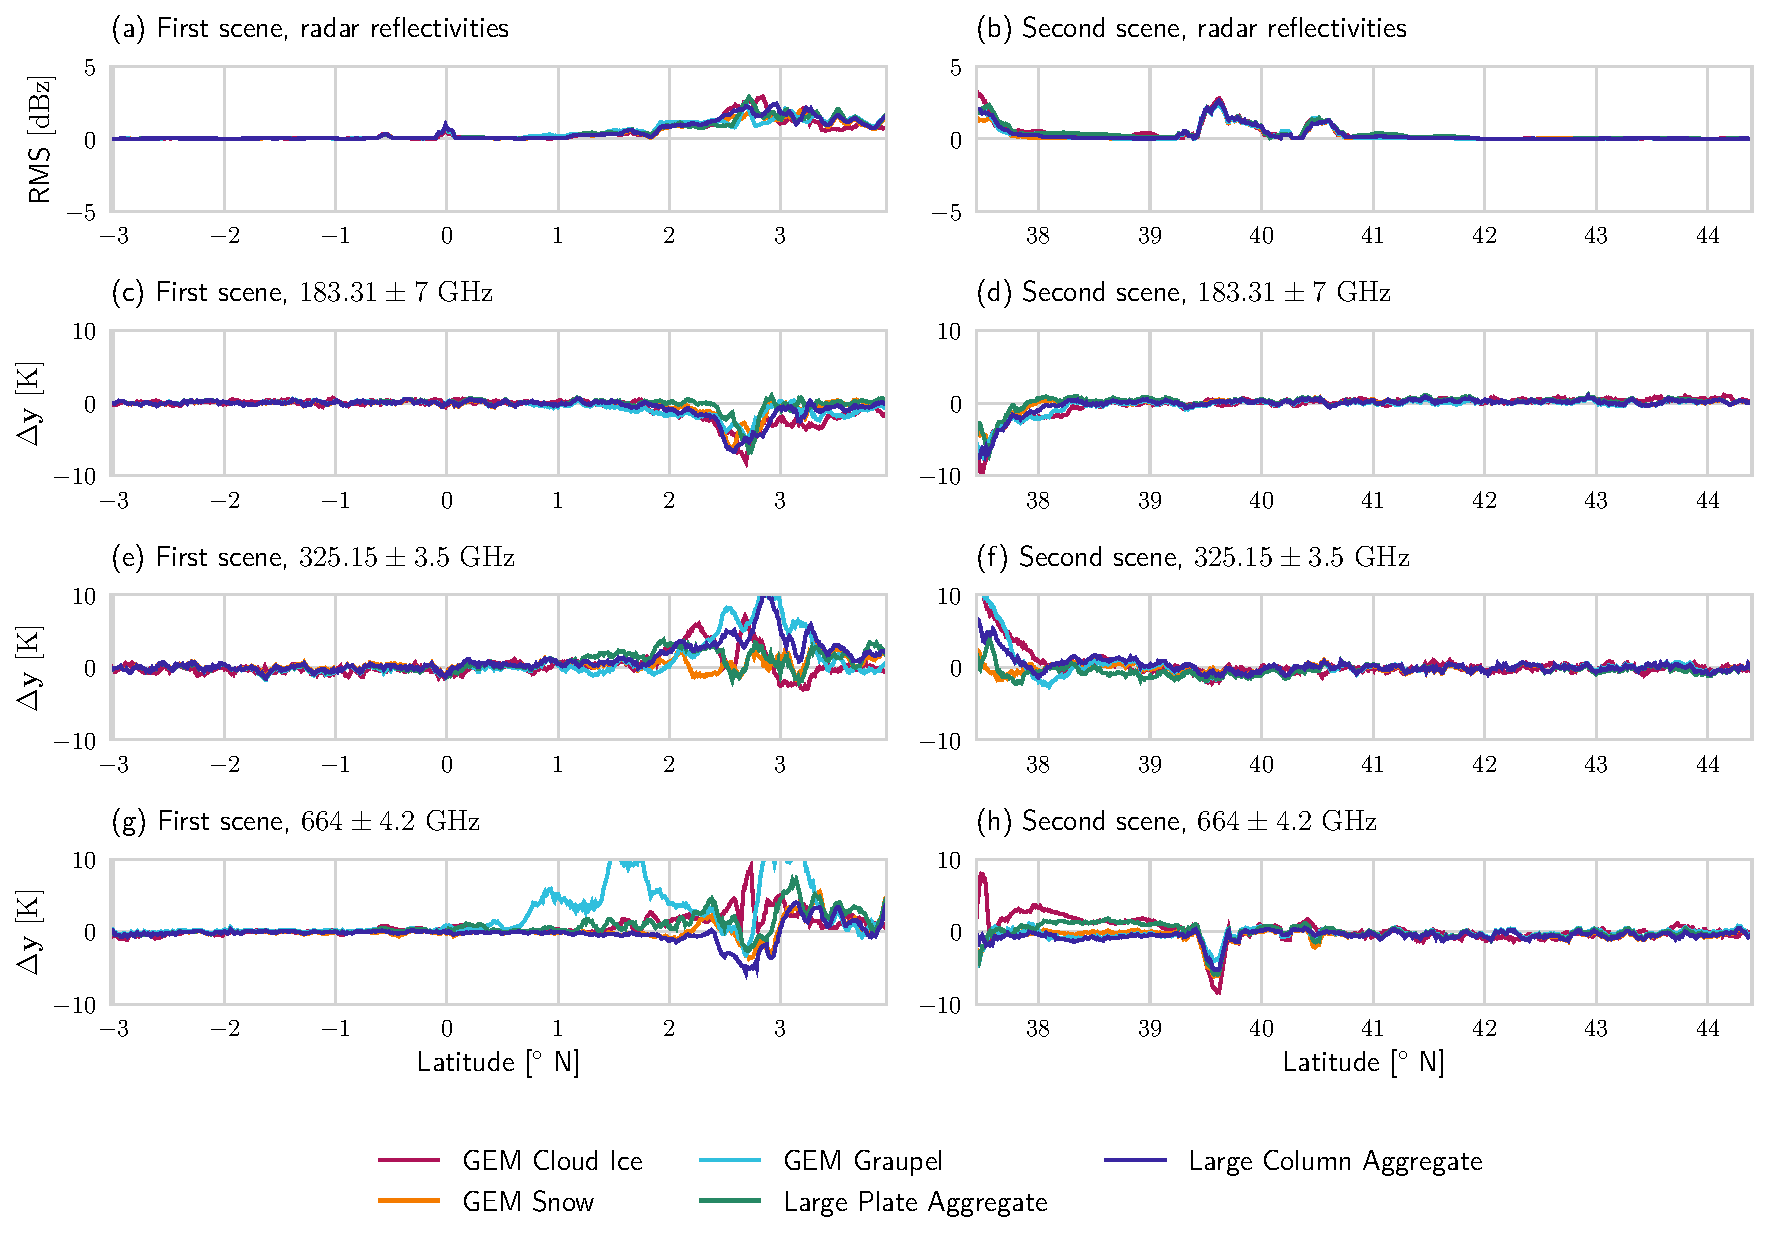
\includegraphics[width = 0.8\textwidth]{../plots/misfits}
\DIFaddendFL \caption{\DIFdelbeginFL \DIFdelFL{Mass-size relations (Panel }\DIFdelendFL \DIFaddbeginFL \DIFaddFL{Residuals of the fitted observations. First row of panels shows the
  profile root mean squared error }\DIFaddendFL (\DIFdelbeginFL \DIFdelFL{a}\DIFdelendFL \DIFaddbeginFL \DIFaddFL{RMS}\DIFaddendFL ) \DIFaddbeginFL \DIFaddFL{between fitted and ($\mathbf{y}_f$}\DIFaddendFL ) and
  \DIFdelbeginFL \DIFdelFL{$\chi^2_y$ values }\DIFdelendFL \DIFaddbeginFL \DIFaddFL{true ($\mathbf{y}$) radar observations }\DIFaddendFL for the two test scenes\DIFdelbeginFL \DIFdelFL{(Panel (b) and (c))}\DIFdelendFL . \DIFdelbeginFL \DIFdelFL{The final cost curves where smoothed using a
  running average filter of }\DIFdelendFL \DIFaddbeginFL \DIFaddFL{Rows 2, 3 and
  4 show the residual $\Delta \mathbf{y} = \mathbf{y}_r - \mathbf{y}$ for }\DIFaddendFL a
  \DIFdelbeginFL \DIFdelFL{width }\DIFdelendFL \DIFaddbeginFL \DIFaddFL{selection }\DIFaddendFL of \DIFdelbeginFL \DIFdelFL{20 profiles}\DIFdelendFL \DIFaddbeginFL \DIFaddFL{ICI channels}\DIFaddendFL .}
\DIFdelbeginFL %DIFDELCMD < \label{fig:costs}
%DIFDELCMD < %%%
\DIFdelendFL \DIFaddbeginFL \label{fig:misfit}
\DIFaddendFL \end{figure}

\subsubsection{Humidity and cloud water}

The developed passive and combined retrieval algorithms also retrieve profiles
of \DIFdelbegin \DIFdel{humidity and liquid cloud mass density. For relative humidity}\DIFdelend \DIFaddbegin \DIFadd{RH and LCWC. For RH}\DIFaddend , both retrievals demonstrate sensitivity but no
improvement \DIFdelbegin \DIFdel{could be }\DIFdelend \DIFaddbegin \DIFadd{was }\DIFaddend observed in the results of the combined retrieval compared to
the passive-only retrieval.
\DIFdelbegin \DIFdel{Moreover, no suitable retrieval setup was found within the scope of this study
which would yield throughout satisfactory performance. Since we do not consider
our results representative of what could be achieved with the observational
approach, they are not included here.
}\DIFdelend 

\DIFdelbegin \DIFdel{The liquid cloud retrieval, however, revealed an additional synergy of the radar
and passive microwave observations. The retrieval
results are therefore }\DIFdelend \DIFaddbegin \DIFadd{For the retrieved LCWC, however, the combined retrieval yields slightly improved
results compared to the passive-only retrieval. Results of the LCWC retrieval
are }\DIFaddend shown in Fig.~\ref{fig:results_cw_b}\DIFdelbegin \DIFdel{to serve as a preview for potential additional
applications of the combined retrieval approach. Panel~(a) of the figure shows
the reference and retrieved column-integrated LWC, here referred to as liquid }\DIFdelend \DIFaddbegin \DIFadd{. The improvements are observed mostly
in the retrieved liquid cloud }\DIFaddend water path (\DIFdelbegin \DIFdel{LWP) . Although the total LWC is still underestimated, the combined
observations clearly improve the LWP retrieval in all regions except those covered
by thick clouds.
}%DIFDELCMD < 

%DIFDELCMD < %%%
\DIFdel{Panel (b) displays the reference LWC drawn as contours on top of the
total
hydrometeor content. Panel (c) and (d) show the retrieved LWC drawn on top of the
retrieved IWC for the passive-only and the combined retrieval. These results
show clearly that the combined retrieval is able to detect and retrieve liquid
clouds even when they overlap with ice clouds. Although some sensitivity of the passive-only retrieval to LWC can be observed as well, the retrieval puts the
cloud too high in the troposphere and underestimates its LWC. This indicates
that the radar reflectivity profile contains useful information for the
retrieval to better locate cloud water in }\DIFdelend \DIFaddbegin \DIFadd{LCWP) in }\DIFaddend the \DIFdelbegin \DIFdel{atmospheric column}\DIFdelend \DIFaddbegin \DIFadd{northern part of the
scene. In particular, it should be noted that the cloud in this part of the
scene is a mixed-phase cloud and that both retrievals successfully retrieve IWC
and LCWC. At the center of the scene both retrievals fail to retrieve
the LCWC. The reason for this is that in these regions rain is present, whose
signal likely swamps any signal from the liquid cloud droplets}\DIFaddend .

\begin{figure}
\centering
\DIFdelbeginFL %DIFDELCMD < \includegraphics[width = \textwidth]{figures/fig16}
%DIFDELCMD < %%%
\DIFdelendFL \DIFaddbeginFL 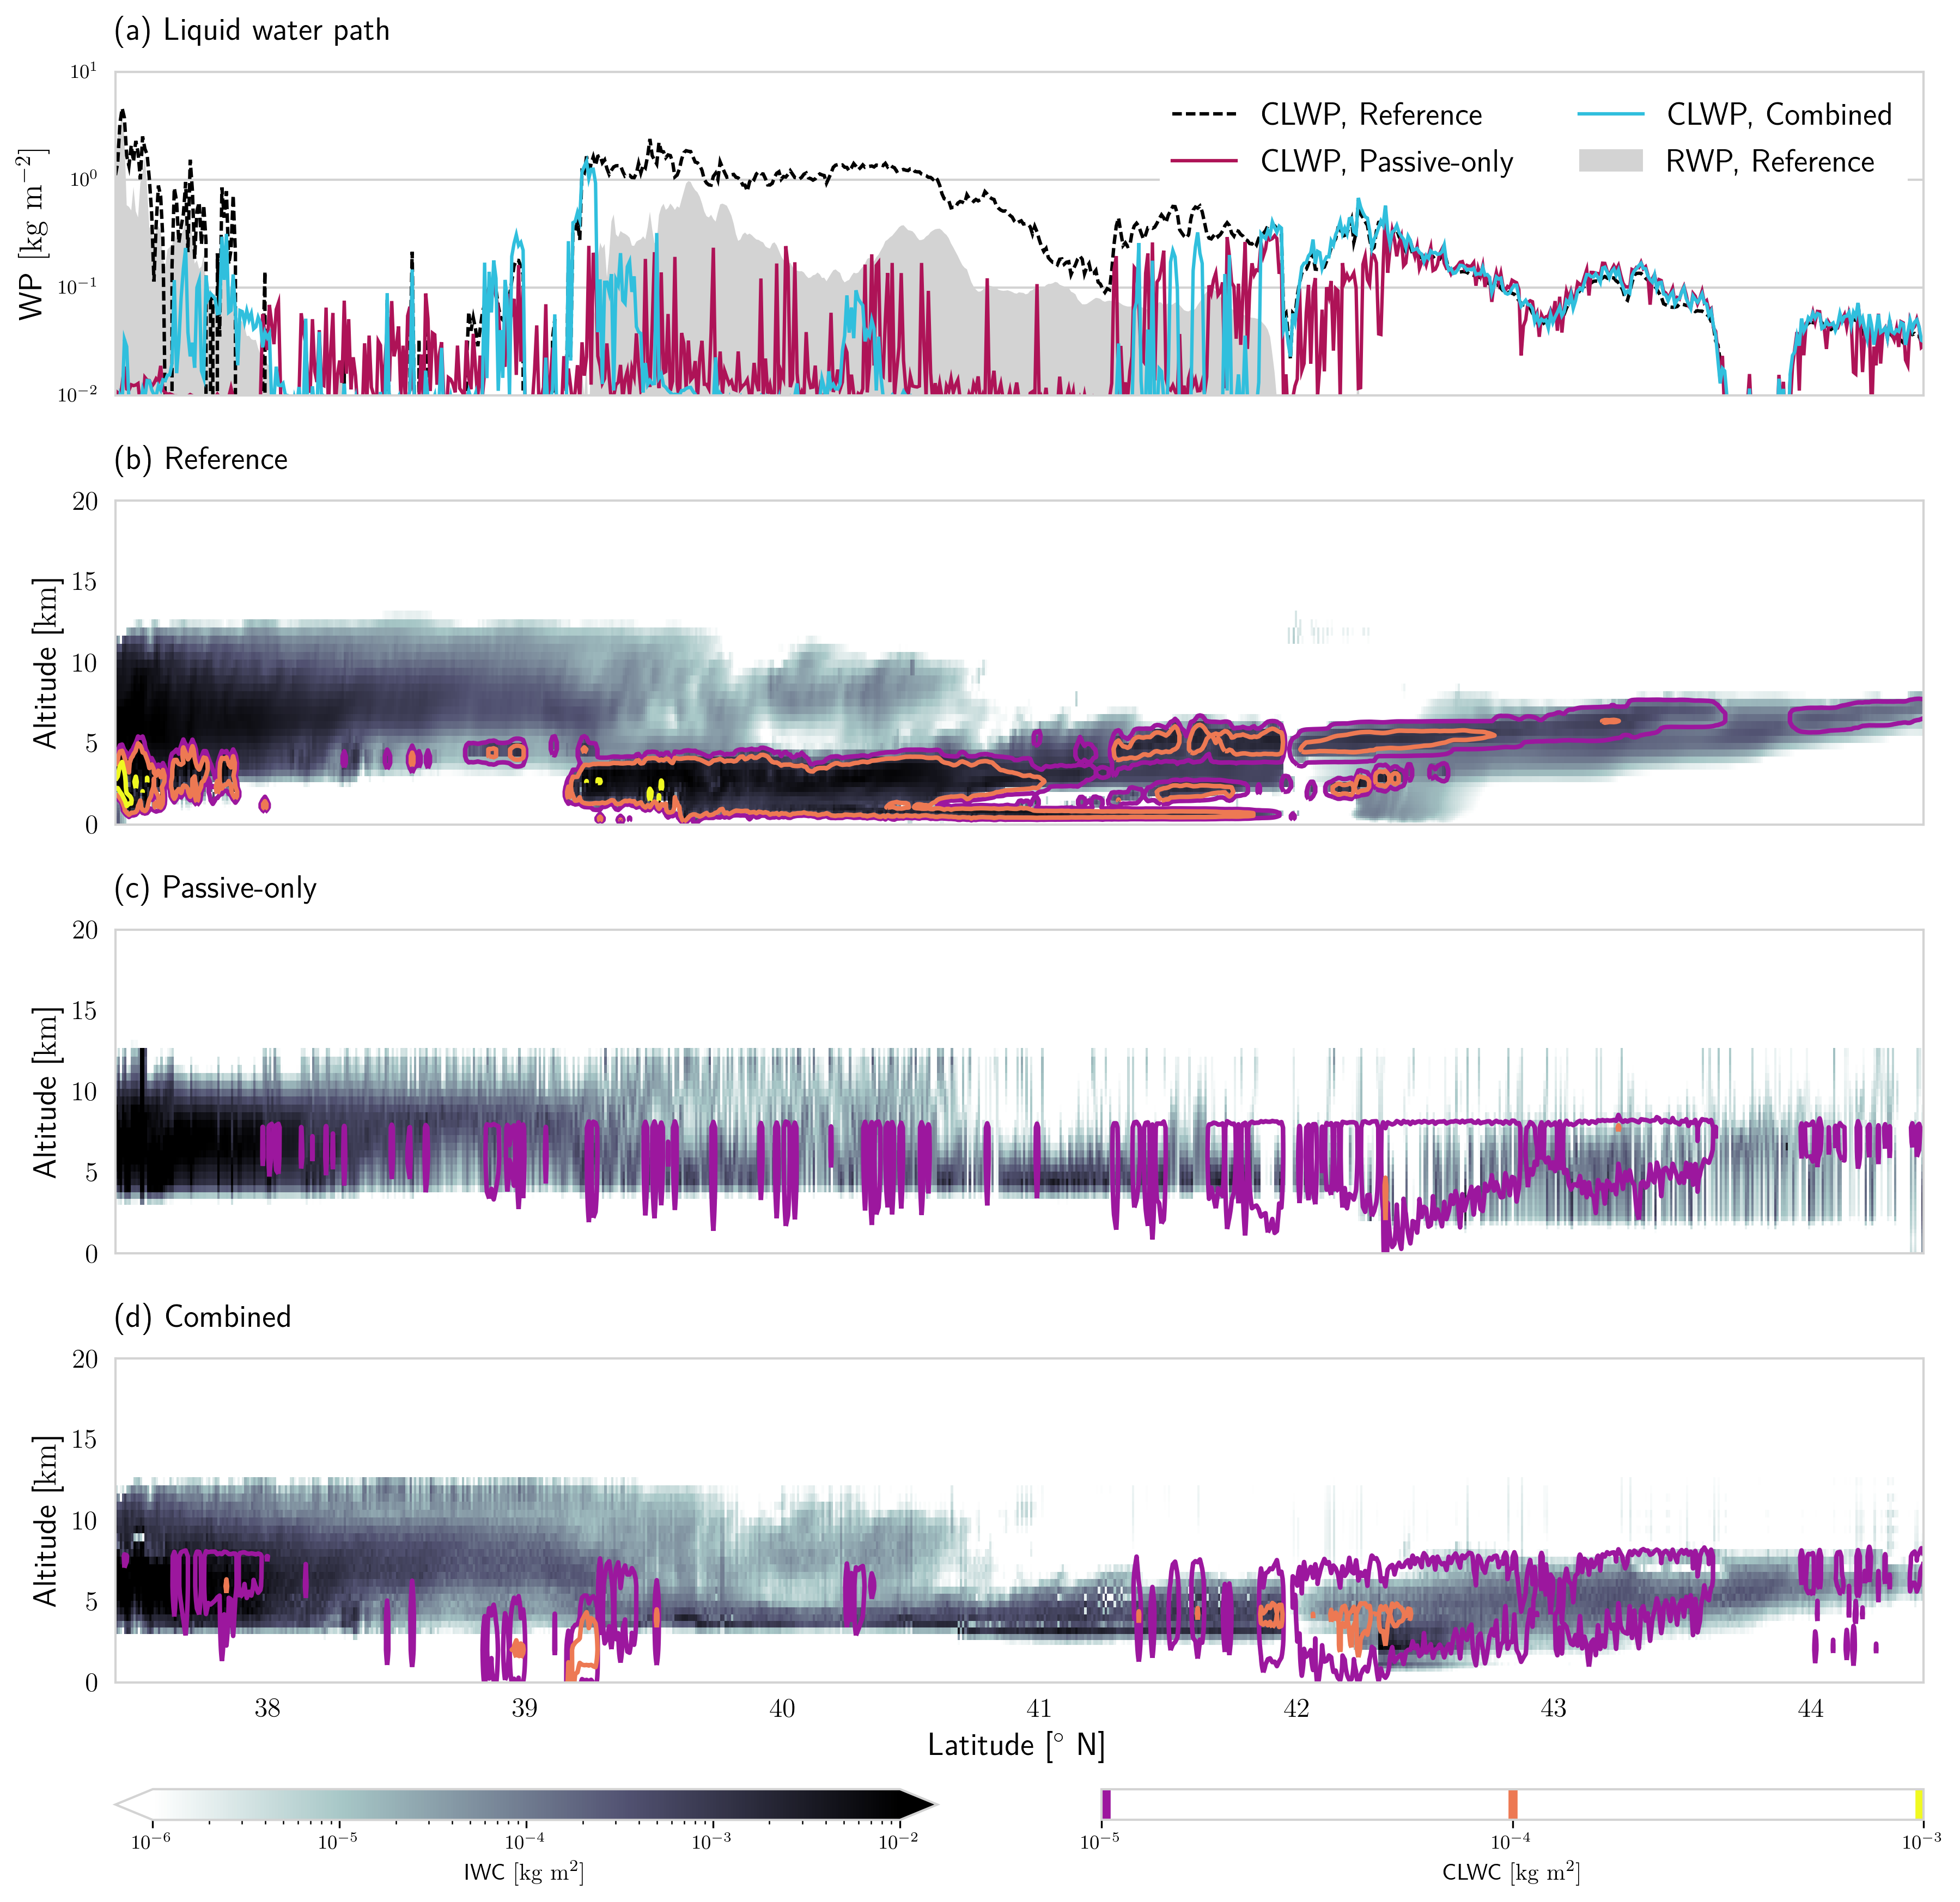
\includegraphics[width = \textwidth]{../plots/results_cw_b_LargePlateAggregate}
\DIFaddendFL \caption{Reference and retrieved \DIFdelbeginFL \DIFdelFL{LWC}\DIFdelendFL \DIFaddbeginFL \DIFaddFL{CLWC and IWC}\DIFaddendFL . Panel (a) shows the reference and
  retrieved LWP for each profile. Panel (b) displays reference LWC contours
  drawn on top of the total hydrometeor content. Retrieval results for
  passive-only and combined retrieval are given in Panel (c) and (d).}
\label{fig:results_cw_b}
\end{figure}


\section{Discussion}
\label{sec:discussion}

The principal aim of this study was to investigate the synergies between radar
and passive sub-millimeter observations \DIFaddbegin \DIFadd{for the retrieval of frozen
hydrometeors}\DIFaddend . To this end, a simplified numerical experiment has been presented,
\DIFdelbegin \DIFdel{that qualitatively }\DIFdelend \DIFaddbegin \DIFadd{which }\DIFaddend demonstrates the existence of complementary information in the radar and
passive microwave observations. Furthermore, a combined retrieval algorithm has
been developed to demonstrate the feasibility of the synergistic \DIFdelbegin \DIFdel{retrievals }\DIFdelend \DIFaddbegin \DIFadd{retrieval }\DIFaddend and
further explore their potential as well as current limitations.

\DIFaddbegin \DIFadd{The novelty of this work lies, for one part, in the application of ICI's
sub-millimeter channels, which sets it apart from the combined retrievals
developed for the TRMM and GPM missions. For the other part, it lies in the
development of a fully-consistent variational retrieval in which all retrieval
quantities are retrieved from the observations from all sensors simultaneously.
This allows comparing the retrieval to equivalent radar-only and passive-only
configurations and therefore a direct analysis of the synergies between the
active and passive observations.
}

\DIFaddend \subsection{Fundamental synergies}

The experiment presented in the first part of this study aimed to \DIFdelbegin \DIFdel{establish }\DIFdelend \DIFaddbegin \DIFadd{illustrate }\DIFaddend the
fundamental synergies of the active and passive microwave observations. It
compared the cloud signals observed by a radar, a millimeter-wave radiometer and
a sub-millimeter-wave radiometer. The results \DIFdelbegin \DIFdel{show }\DIFdelend \DIFaddbegin \DIFadd{indicate }\DIFaddend that the combined
observations can simultaneously constrain the \DIFdelbegin \DIFdel{horizontal and vertical scaling of
the particle size distribution}\DIFdelend \DIFaddbegin \DIFadd{size and concentration of
particles in the cloud}\DIFaddend . However, the complementary information content between
the active and passive observations depends on both the properties of the
observed cloud and the frequency of the observations. For the lower frequencies
considered in this study, i.e. the highest channels of the MWI radiometer, the
regions where both observations provide complementary information on the
particle size distribution of the cloud are limited to very high \DIFdelbegin \DIFdel{mass densities }\DIFdelend \DIFaddbegin \DIFadd{water content
}\DIFaddend and particle sizes. It should be noted, however, that since the radar
simulations neglect multiple scattering, \DIFdelbegin \DIFdel{the results are likely less
accurate in this region of the cloud-parameter space}\DIFdelend \DIFaddbegin \DIFadd{these results may not necessarily
carry over to space-borne observations}\DIFaddend . As the passive observing frequency
increases, the regions of complementary information content extend down to
smaller particle sizes and \DIFdelbegin \DIFdel{cloud mass density}\DIFdelend \DIFaddbegin \DIFadd{water content}\DIFaddend . Especially the highest-frequency
channels of the ICI radiometer can therefore be expected to provide
\DIFdelbegin \DIFdel{additional information on the particle size distribution of ice clouds}\DIFdelend \DIFaddbegin \DIFadd{complementary information to a W-band radar in a combined observation
scenario}\DIFaddend .

\subsection{Combined cloud retrieval}

In the second part of the study, we have presented results from a combined,
variational cloud retrieval applied to synthetic observations from two test
scenes from a high-resolution atmosphere model. The results of the combined
retrieval were compared to that of a passive- and a radar-only version of the
retrieval algorithm. The simulated observations \DIFaddbegin \DIFadd{assumed an airborne viewing
geometry and therefore }\DIFaddend neglected potential errors caused by different or
non-overlapping antenna beams as well as inhomogeneity of the atmosphere across
the beams. On the other hand, a source of forward model error was included by
applying a more complex microphysics scheme in the simulations than the one used
in the retrieval. This allows assessing the retrieval error caused by the
simplified modeling of cloud microphysics in the retrieval.

\subsubsection{Retrieval performance}

Of the three considered retrieval implementations, the passive-only retrieval
clearly performs worst in terms of retrieved IWC. It should be noted, however,
that the passive only retrieval presented here has not been fully optimized and
should therefore not be taken as representative of the potential performance of
the MWI and ICI radiometers for IWC retrievals. To ensure a fair comparison, the
retrieval uses almost the same a priori assumptions as the other two retrievals,
which in the presented case provide only very limited information on the
vertical structure of the cloud. As has been shown also by other studies, the
passive observations do provide information on the vertical distribution of ice
in the atmospheric column \citep{wang17, grutzun18}, but the information content
is limited to a few degrees of freedom. It is therefore unlikely that the
vertical resolution of the passive-only retrieval can be improved drastically
without further constraining it a priori, as it is typically done in retrievals
that use Monte Carlo integration or neural networks \citep{pfreundschuh18}.

With respect to IWP, however, the passive retrieval can perform as well or even
better than the radar-only \DIFdelbegin \DIFdel{and the combined }\DIFdelend retrieval. Furthermore, the results in
\DIFdelbegin \DIFdel{Figure}\DIFdelend \DIFaddbegin \DIFadd{Fig.}\DIFaddend ~\ref{fig:results_nd_a} indicate that the passive observations provide some
information on the particle number concentrations, which is not the case for the
radar observations. This in itself is an interesting result as it shows that
even when considered separately, observations from active and passive microwave
sensors should be considered complementary to each other in their information
content.

As expected, the radar-only retrieval provides much better IWC retrievals than
the passive-only version. However, the results \DIFaddbegin \DIFadd{of the two-moment retrieval
}\DIFaddend exhibit systematic deviations from the reference values in certain regions of
the cloud. The analysis of the retrieval performance shown in
\DIFdelbegin \DIFdel{Figure~\ref{fig:results_scatter_a_1},
\ref{fig:results_scatter_a_2} and \ref{fig:results_scatter_b_1} }\DIFdelend \DIFaddbegin \DIFadd{Fig.~\ref{fig:results_scatter_a} and \ref{fig:results_scatter_b} }\DIFaddend revealed that
these are caused by systematic errors in the retrieval of specific hydrometeor
species from the GEM model. \DIFdelbegin \DIFdel{A likely explanation for this is that the priori
assumptions applied }\DIFdelend \DIFaddbegin \DIFadd{Interestingly, the 1M version of the radar only
retrieval did not produce the large errors in the second scene but therefore
produced systematic errors for the first test scene. This indicates that the a
priori assumptions used }\DIFaddend in the retrieval do not \DIFdelbegin \DIFdel{fit the specific microphysical
properties of the species in the model. This hypothesis is confirmed by the
radar-retrieved number density fields shown in Fig.~\ref{fig:results_nd_a} and Fig.~\ref{fig:results_nd_scatter_a}. While the reference distribution has two
modes corresponding to ice and snow, the retrieved values are nearly the same
throughout the whole scene.
Viewed }\DIFdelend \DIFaddbegin \DIFadd{provide a sufficiently well
description of how the $D_m$ and $N_0^*$ parameters of the PSD co-vary and that
the radar-only observations alone do not constrain both of them well enough.
This is plausible also }\DIFaddend from an information content perspective \DIFdelbegin \DIFdel{, this
is plausible }\DIFdelend since the radar
provides only one piece of independent information at each range gate, which is
insufficient to determine the two degrees of freedom ($N_0^*$ and $D_m$) of the
PSD. \DIFdelbegin \DIFdel{The information on the second degree of
freedom must therefore come from the a priori assumptions.
}%DIFDELCMD < 

%DIFDELCMD < %%%
\DIFdel{The a priori assumptions which were used in this study were similar but not
identical to what is  used in the DARDAR retrievals. Also here it should be
noted, that the presented results should not be taken to be representative for
the DARDAR product.Rather than this, the DARDAR a priori settings were chosen
since they represent well established and validated assumptions for ice cloud
retrievals and therefore should provide a reasonable starting point for the
development of a combined cloud retrieval.The fact that the a priori
assumptions used in the DARDAR retrieval do not agree with the microphysical
properties of }\DIFdelend \DIFaddbegin \DIFadd{This hypothesis is  confirmed by the radar-retrieved number density fields shown
in Fig.~\ref{fig:results_nd_a} and Fig.~\ref{fig:results_nd_scatter_a}. While
the distribution of reference values has two modes corresponding to }\DIFaddend ice and
snow\DIFdelbegin \DIFdel{in the GEM model, does not say much about the general
validity of these assumptions}\DIFdelend \DIFaddbegin \DIFadd{, the retrieved values are nearly the same throughout the whole scene
indicating that the observations themselves provide almost no information on
particle concentrations}\DIFaddend .

Despite \DIFdelbegin \DIFdel{the }\DIFdelend certain visible artifacts in the retrieved IWC field (Fig.
\ref{fig:results_a}), the analysis of the results of the combined retrieval
presented in \DIFdelbegin \DIFdel{Figs.~\ref{fig:results_scatter_a_1} , \ref{fig:results_scatter_a_2}
}\DIFdelend \DIFaddbegin \DIFadd{Fig.~\ref{fig:results_scatter_a} }\DIFaddend and in particular
\DIFaddbegin \DIFadd{Fig.~}\DIFaddend \ref{fig:boxes} shows that it yields, at least for most of the tested
particle models, the best retrieval performance for IWC and IWP. The benefit of
the combined observations is even more pronounced in the retrieved number
density fields (Fig.~\ref{fig:results_nd_a}). Here, the passive- and radar-only
\DIFdelbegin \DIFdel{retrieval }\DIFdelend \DIFaddbegin \DIFadd{retrievals }\DIFaddend showed little to no skill in retrieving the particle number
concentrations. \DIFdelbegin \DIFdel{The combined retrieval , however, }\DIFdelend \DIFaddbegin \DIFadd{In contrast to this, the combined retrieval }\DIFaddend was able to
reproduce the general structure of the number concentration fields in regions
where the cloud composition is homogeneous
(Fig.~\ref{fig:results_nd_scatter_a}). In particular this \DIFdelbegin \DIFdel{showed }\DIFdelend \DIFaddbegin \DIFadd{shows }\DIFaddend that the
combined retrieval is able to distinguish the microphysical properties of ice
and snow in the model. \DIFdelbegin %DIFDELCMD < 

%DIFDELCMD < %%%
\subsubsection{\DIFdel{Impact of the assumed particle shape}}
%DIFAUXCMD
\addtocounter{subsubsection}{-1}%DIFAUXCMD
%DIFDELCMD < 

%DIFDELCMD < %%%
\DIFdel{Although }\DIFdelend \DIFaddbegin \DIFadd{Instead of relying on the a priori, }\DIFaddend the combined
retrieval can \DIFdelbegin \DIFdel{reduce systematic errors in the retrieved
IWC and IWP, its performance can even degrade if an unrealistic particle habit
is used, as observed }\DIFdelend \DIFaddbegin \DIFadd{use information from the observations to constrain the cloud
microphysics, which avoids the systematic errors observed in the radar-only
retrievals.
}

\DIFadd{The a priori assumptions used in this study are similar to those of the DARDAR-CLOUD
product, since they represent well established and validated assumptions for ice
cloud retrievals. The role of the a priori is to complement the observations
with additional information required to make the retrieval problem tractable.
For the hydrometeor retrieval this means that the a priori determines how the
information from the observations, which alone is insufficient to accurately
determine both degrees of freedom of the PSD, is distributed between its $D_m$
and $N_0^*$ parameters. For the radar-only retrieval, this works well for cloud
systems containing both ice and snow but leads to biased retrievals in both IWC
and IWP when this is not the case, as seen }\DIFaddend in Fig.~\ref{fig:boxes}. \DIFdelbegin \DIFdel{In general,
the passive-only and the combined retrievals display }\DIFdelend \DIFaddbegin \DIFadd{Of course,
the DARDAR product also makes use of co-located lidar observations, so this 
would not effect observations where both radar and lidar overlap. However,
our results indicate that by combining radar and passive microwave observations
the microphysical properties of hydrometeors can be constrained even deeper
inside clouds, where optical or infrared sensors would not provide any
information.
}

\subsubsection{\DIFadd{Impact of the assumed particle shape}}

\DIFadd{Our experiments show a }\DIFaddend stronger sensitivity to the assumed \DIFdelbegin \DIFdel{particle shape
}\DIFdelend \DIFaddbegin \DIFadd{ice particle shape
for the passive-only and the combined retrievals }\DIFaddend than the radar-only retrieval.
\DIFdelbegin \DIFdel{This is plausible since the }\DIFdelend \DIFaddbegin \DIFadd{The passive observations probe the particle at multiple frequencies and their
}\DIFaddend increased sensitivity especially of the sub-millimeter radiometer channels has
been highlighted in several studies \DIFdelbegin \DIFdel{\mbox{%DIFAUXCMD
\citep{ekelund19a, fox19}}\hspace{0pt}%DIFAUXCMD
}\DIFdelend \DIFaddbegin \DIFadd{\mbox{%DIFAUXCMD
\citep{ekelund20, fox19}}\hspace{0pt}%DIFAUXCMD
}\DIFaddend .

\DIFdelbegin \DIFdel{Given the increased sensitivity of the passive-only and combined retrieval to
}\DIFdelend \DIFaddbegin \DIFadd{Only the combined retrieval was able to yield accurate IWC retrievals for both
test scenes for suitable choices of the particle model. However, if an
unsuitable particle shape is chosen, }\DIFaddend the \DIFdelbegin \DIFdel{assumed particle shape , it would be desirable to know which of the properties of a particle model are most critical for its representativeness. Five
different particle models were tested here: The two most dominant from
the GEM model and three additional models taken from the ARTS SSDB. The two GEM particles both showed the worst retrieval performance.For the
GemCloudIce model}\DIFdelend \DIFaddbegin \DIFadd{induced errors may actually outweigh
the benefits of the combined retrieval as is the case for the Large Column
Aggregate and the GEM Cloud Ice shapes (Fig.~\ref{fig:boxes}). Judging from the
particle properties displayed in Fig.~\ref{fig:particle_properties}}\DIFaddend , a likely
explanation for \DIFdelbegin \DIFdel{its bad performance is its very high density. The GemSnow model
has similar density as the 8-ColumnAggregate, but does not reach down to small
particle sizes, possibly explaining why it is unsuitable for the retrieval }\DIFdelend \DIFaddbegin \DIFadd{the good performance of the Large Plate Aggregate and the GEM
Graupel particle is that their properties are intermediate to those of GEM Cloud
Ice and GEM Snow, which are the dominating shapes in the test scenes. Provided
that the hydrometeors of the GEM model and their assumed particle properties are
sufficiently realistic to model real observations, this would mean that accurate
IWC retrievals can be achieved using only a single hydrometeor species with
suitable scattering properties that are intermediate to snowflake-type and
heavily rimed particles. This is in agreement with \mbox{%DIFAUXCMD
\citet{ekelund20} }\hspace{0pt}%DIFAUXCMD
who found
the Large Plate Aggregate to to yield good agreement with observations from the
GPM Microwave Imager at $190\ \unit{GHz}$}\DIFaddend .
\DIFdelbegin \DIFdel{Nonetheless, small performance differences are observed also for the other three
models}\DIFdelend \DIFaddbegin 

\DIFadd{The analysis of the residuals of the retrieval fit (Fig.~\ref{fig:misfit})
showed that the residuals for different particle shapes differ most where the
cloud is thick. Differences between different particles are observed}\DIFaddend , but no
\DIFdelbegin \DIFdel{clear connection to their mass-size relation }\DIFdelend \DIFaddbegin \DIFadd{relationship to the retrieval accuracy in terms of IWC }\DIFaddend can be established. \DIFdelbegin \DIFdel{This indicates that also its specific scattering properties are important factors
that determine representativeness of a particlemodel.
}%DIFDELCMD < 

%DIFDELCMD < %%%
\DIFdel{Furthermore, it has been briefly investigated whether the goodness of the
fit to
the observations can provide information on the suitability of
the chosen
particle model. In particular, we aimed to address the question whether the combined observations can constrain the dominant particle shape or whether a
good fit to the
observations can be obtained }\DIFdelend \DIFaddbegin \DIFadd{The
GEM Graupel particle, for example, yields accurate IWC retrievals but gives the
worst fit for the first test scene. A likely explanation for this is that the
retrieved IWC depends mostly on the efficiency with respect to water content of
the interaction between the particle and the radiation, whereas the retrieval
residual is likely due to the relative efficiencies at different frequencies.
Moreover, in the remaining parts of the scenes, there are no differences in the
residuals for different particles. This means that the retrieval can fit the
observations well }\DIFaddend regardless of the \DIFdelbegin \DIFdel{applied particle model. Unfortunately, no evidence of a relation between the $\chi^2_y$ value and the retrieval performance was observed. It thus remains an open question whether
and how information on }\DIFdelend \DIFaddbegin \DIFadd{assumed particle shape and indicates that
the observations alone do not constrain the particle shape. This indicates that
}\DIFaddend the ice particle shape \DIFdelbegin \DIFdel{can be extracted from microwave
observations of ice particles}\DIFdelend \DIFaddbegin \DIFadd{is not constrained by the observations and must be
determined a priori}\DIFaddend .

\subsubsection{Humidity and cloud water}

As an outlook, \DIFdelbegin \DIFdel{we have also included }\DIFdelend \DIFaddbegin \DIFadd{also }\DIFaddend results from the \DIFdelbegin \DIFdel{liquid cloud retrieval ,
that clearly shows its capability to retrieve liquid cloud mass densities even
within mixed-phase clouds.
Although certain sensitivity to cloud water is
observed also for }\DIFdelend \DIFaddbegin \DIFadd{LCWC retrieval have been provided.
Fig.~\ref{fig:results_cw_b} shows improvements in retrieved LCWP and LCWC in the
results of the combined retrieval compared to }\DIFaddend the passive-only \DIFdelbegin \DIFdel{retrieval, }\DIFdelend \DIFaddbegin \DIFadd{retrieval.
Although also }\DIFaddend the \DIFdelbegin \DIFdel{addition of the radar signal
clearly improved the localization of the cloud in the atmosphere. This explains
the observed improvement in the retrieved LWP, since at lower altitude a thicker
cloud is required to yield the same passive cloud signal}\DIFdelend \DIFaddbegin \DIFadd{passive-only retrieval shows sensitivity to LCWC, the results
are less stable than those of the combined retrieval}\DIFaddend . This shows that
\DIFdelbegin \DIFdel{combined radar
and microwave radiometer observationscan also }\DIFdelend \DIFaddbegin \DIFadd{sub-millimeter radiometers, in particular in combination with radar
observations, can }\DIFaddend be used for \DIFdelbegin \DIFdel{the
profiling of warm and supercooled liquid clouds}\DIFdelend \DIFaddbegin \DIFadd{retrieving both frozen and liquid cloud water
content in mixed-phase clouds. This conclusion is supported by the information
content analysis in Fig.~\ref{fig:dfs}, which shows that the passive
observations provide a small amount of information on liquid clouds and that
this is increased for the combined retrieval}\DIFaddend .

\DIFdelbegin \DIFdel{Although no satisfactory results were obtained from the water vapor retrieval,
the retrieval results still indicate sensitivity of this setup for retrieving
atmospheric humidity.The full exploration of the potential of the combined
observations for liquid cloud and water vapor is out of the scope of this study
and is left to future investigation.
}%DIFDELCMD < 

%DIFDELCMD < %%%
\subsubsection{\DIFdel{Retrieval method}}
%DIFAUXCMD
\addtocounter{subsubsection}{-1}%DIFAUXCMD
%DIFDELCMD < 

%DIFDELCMD < %%%
\DIFdel{The combined retrievalimplementation showed robust performance on fairly
distinct and complex cloud scenes.
Despite this, both scenes that were
considered here contained parts where the OEM minimization did not find a state
that results in a good fit to the observations. In contrast to that, the radar-only retrievaldid converge well in most regions where the final cost of
}\DIFdelend \DIFaddbegin \DIFadd{For the water vapor retrieval, no significant improvements in }\DIFaddend the combined
retrieval \DIFdelbegin \DIFdel{remained high. The inability of the retrieval to fit the observations indicates additional information that is contained in }\DIFdelend \DIFaddbegin \DIFadd{results were observed and also the analysis of the information content
does not show any increase in information content. This indicates that }\DIFaddend the
combined observations \DIFdelbegin \DIFdel{but which the retrieval method cannot disentangle. Furthermore, the
results exhibit visible profile-to-profile variability as well as some artifacts
in the form of
high-frequency vertical oscillation.
We have tried to
counteract
these by increasing the vertical spatial correlation but to no avail. }\DIFdelend \DIFaddbegin \DIFadd{do not provide any synergies for the retrieval of
humidity.
}\DIFaddend 

\DIFdelbegin \DIFdel{This raises the question of the suitability of the OEM method applied here . The
combined retrieval violates the two fundamental assumptions of the OEM method: The forward model is non-linear and the assumed Gaussian }\DIFdelend %DIF > \subsubsection{Retrieval method}
%DIF > 
%DIF > The combined retrieval implementation showed robust performance on fairly
%DIF > distinct and complex cloud scenes. Despite this, both scenes that were
%DIF > considered here contained parts where the OEM minimization did not find a state
%DIF > that results in a good fit to the observations. In contrast to that, the
%DIF > radar-only retrieval did converge well in most regions where the final cost of
%DIF > the combined retrieval remained high. The inability of the retrieval to fit the
%DIF > observations indicates additional information that is contained in the combined
%DIF > observations but which the retrieval method cannot disentangle. Furthermore, the
%DIF > results exhibit visible profile-to-profile variability as well as some artifacts
%DIF > in the form of high-frequency vertical oscillation. We have tried to counteract
%DIF > these by increasing the vertical spatial correlation but to no avail.
%DIF > 
%DIF > This raises the question of the suitability of the OEM method applied here. The
%DIF > combined retrieval violates the two fundamental assumptions of the OEM method:
%DIF > The forward model is non-linear and it is difficult to describe the variability
%DIF > of cloud parameters using Gaussian a priori assumptions. In addition to that,
%DIF > the current implementation of the retrieval is computationally very expensive.
%DIF > For further development of the combined retrieval concept it may therefore be
%DIF > advisable to revisit the applied retrieval method in search for a potentially
%DIF > more suitable alternative.
%DIF > 
%DIF > Some of the above-mentioned problems could likely be counteracted by accounting
%DIF > for the forward model error caused by the simplified forward model applied in
%DIF > the retrieval. However, finding an accurate description of this error
%DIF > would require developing a suitable model for it which was deemed out of the
%DIF > this studies' scope.
\DIFaddbegin 

\subsubsection{\DIFadd{Limitations}}

\DIFadd{An important limitation of this study is its scope: The aim here was not to
develop a production-ready combined retrieval product but rather a
proof-of-concept to explore this observational approach. The retrieval results
presented here should therefore not be interpreted in absolute terms. The
primary results are based on the relative performances of the three retrieval
methods: Given equivalent }\DIFaddend a priori assumptions\DIFdelbegin \DIFdel{do
not describe reality very well. In addition to that, the current implementation
of the retrieval is computationally very expensive. For further development of
the combined retrieval
concept it may therefore be advisable to revisit the applied retrieval method in search for a potentially more suitable alternative}\DIFdelend \DIFaddbegin \DIFadd{, the combined retrieval
demonstrates higher sensitivity to the microphysical properties than the
radar-only retrieval and lower errors in terms of IWC than the passive-only
retrieval}\DIFaddend .

\DIFdelbegin \subsubsection{\DIFdel{Limitations}}
%DIFAUXCMD
\addtocounter{subsubsection}{-1}%DIFAUXCMD
%DIFDELCMD < 

%DIFDELCMD < %%%
\DIFdel{Finally, it is important to consider the limitations }\DIFdelend \DIFaddbegin \DIFadd{Another limiting factor }\DIFaddend of this study \DIFdelbegin \DIFdel{. The results
presented here are }\DIFdelend \DIFaddbegin \DIFadd{are that it is }\DIFaddend purely based on simulations
and restricted to two selected model test scenes. The validity of the presented
results thus \DIFdelbegin \DIFdel{to some extent
}\DIFdelend depends on how well cloud microphysics are represented in \DIFaddbegin \DIFadd{the }\DIFaddend GEM
model. While this may \DIFdelbegin \DIFdel{affect the specific performance results for the tested retrieval methods}\DIFdelend \DIFaddbegin \DIFadd{again affect an interpretation of the results in absolute
terms}\DIFaddend , the main findings of this work, \DIFdelbegin \DIFdel{namely that the combined retrieval shows greater
sensitivity to the microphysical properties of ice hydrometeors than the radar-
or passive-only retrievals}\DIFdelend \DIFaddbegin \DIFadd{which are based on a relative comparison
of the retrieval results}\DIFaddend , should be independent of the realism of the test
scenes.

\DIFdelbegin \DIFdel{Furthermore, the forward simulations used to generate the synthetic observations do not consider beam filling issues, assume a
slightly unrealistic viewing geometry and neglect multiple scattering in the radar simulations. For }\DIFdelend \DIFaddbegin \DIFadd{As has been stated above, simulated observations used in this study assumed a
viewing geometry that is realistic only for airborne observations. They
therefore do not provide }\DIFaddend a realistic assessment of the potential \DIFdelbegin \DIFdel{retrieval performance this should
certainly be taken into account . Again,
it is important to understand the
results presented here as a study of the fundamental synergies of active and
passive microwave observationsrather than an accurate performance assessment of the combined retrieval }\DIFdelend \DIFaddbegin \DIFadd{of a
space-borne satellite mission involving ICI, MWI and a W-band radar. For this it
would be necessary to take into account a more realistic viewing geometry,
beam-filling errors as well as multiple scattering in the radar observations.
Quantifying the effect of these error sources on the retrieval synergies is
left for future investigation}\DIFaddend .

\conclusions  %% \conclusions[modified heading if necessary]
\label{sec:conclusions}

The main \DIFdelbegin \DIFdel{conclusions from the results presented above are:
}%DIFDELCMD < \begin{enumerate}
%DIFDELCMD < \item %%%
\DIFdel{The complementary information in active and
passive microwave observations canconstrain two degrees of freedom of the
PSD }\DIFdelend \DIFaddbegin \DIFadd{conclusion from this work is that the combination of radar and
sub-millimeter radiometer observations can, to some extent, constrain both the
size and number concentration }\DIFaddend of frozen hydrometeors. \DIFdelbegin %DIFDELCMD < \item %%%
\DIFdel{This reduces systematic retrieval errors for specific hydrometeor species whose
  properties are not well described by the a priori assumptions.
}%DIFDELCMD < \item %%%
\DIFdel{Especially the sub-millimeter channels of the ICI radiometer contribute to the synergistic information content for ice particles. }%DIFDELCMD < \end{enumerate}
%DIFDELCMD < 

%DIFDELCMD < %%%
\DIFdel{In addition to this}\DIFdelend \DIFaddbegin \DIFadd{The increased sensitivity
of the combined retrieval to the microphysical properties of hydrometeors can
increase the accuracy of IWC retrievals and avoid systematic errors observed in
an equivalent radar-only retrieval. Moreover}\DIFaddend , the combined retrieval \DIFdelbegin \DIFdel{also shows improved profiling capabilities
for warm and supercooled liquid clouds}\DIFdelend \DIFaddbegin \DIFadd{showed clear
sensitivity to the particle number density and was able reproduce its vertical
structure in regions where the cloud composition is homogeneous}\DIFaddend .

The results \DIFdelbegin \DIFdel{presented in this study }\DIFdelend particularly highlight the \DIFdelbegin \DIFdel{complementarity
of the active and passive observations: Although the radar provides observations
at high vertical resolution, they contain insufficient information on the
microphysical properties of hydrometeors. The passive-only observations , on the
contrary, have low vertical resolution, but are more sensitive to cloud
microphysics allowing a potentially more accurate IWP retrieval than what can be
obtained from the radar alone. A synergistic retrieval using both types of
observations allows combining the high vertical resolution of the radar with the
sensitivity to cloud microphysics of the passive observations, which
yields more accurate retrievals of IWC, IWP and  particle number densities}\DIFdelend \DIFaddbegin \DIFadd{importance of sub-millimeter observations
for combined retrievals of frozen hydrometeors. While observations at currently
available microwave frequencies provide information complementary to that from a
radar only for thick clouds with very large particles ($D_m > 800\ \unit{\mu m},
\text{IWC} > 10^{-4}\ \unit{kg\ m^{-3}}$), frequencies above $200\ \unit{GHz}$
provide additional information on cloud microphysics (Fig.~\ref{fig:contours})
at smaller particles sizes and water content ($D_m > 200\ \unit{\mu m},
\text{IWC} > 10^{-5}\ \unit{kg\ m^{-3}}$).
}

\DIFadd{Regarding the representation of hydrometeors in the retrieval, our results
indicate that complex mixes of hydrometeors can be accurately represented
using a single, suitable habit mix. In particular, our results point towards that
a suitable habit should have scattering properties that are intermediate
between strongly rimed and  more snow-flake like particles}\DIFaddend .

\DIFdelbegin \DIFdel{Synergistic retrievals from active and passive microwave observations ideally
complement currently available observation systems that combine radar with
observations in the visible or infrared. The advantage of combined microwave
observations is that they provide sensitivity throughout the whole cloud,
where
visible and infrared observations would be saturated. Where only information
from the radar is available, a retrieval based on optical or infrared
observations has to rely on a priori assumptions, which may cause similar
systematic errors as what has been observed in this study. In addition to this, our results underline the benefits of ICI's sub-millimeter channels, which significantly improve the sensitivity of the passive observations to smaller
particle sizes and mass densities and thus narrow the sensitivity gap between
the observing frequencies of traditional microwave imagers and observations in the infrared and visible domain. }%DIFDELCMD < 

%DIFDELCMD < %%%
\DIFdel{The upcoming launch of the ICI and MWI radiometers thus }\DIFdelend \DIFaddbegin \DIFadd{A direct application of the synergistic retrieval algorithm developed in this
study are flight campaigns involving the International Sub-millimetre Airborne
Radiometer (ISMAR, \mbox{%DIFAUXCMD
\citet{fox17}}\hspace{0pt}%DIFAUXCMD
) combined for example with a radar on another
aircraft or the Microwave Radar/radiometer for Arctic Clouds (MiRAC,
\mbox{%DIFAUXCMD
\citet{mech19}}\hspace{0pt}%DIFAUXCMD
). The ability of the combined retrieval to constrain two moments
of the PSD of frozen hydrometeors should make it a valuable tool for validating
the representation of clouds in cloud-resolving or large-eddy simulations which
typically employ two-moment schemes. Moreover, since our results indicate
certain retrieval skill also for LCWC in mixed-phase clouds, such
observations can be used to study the properties of these clouds which play an
important role for the climate of the arctic.
}

\DIFadd{Ultimately, spaceborne combined radar/sub-millimeter observations can be a way
forward towards reducing the large uncertainties in the observational record of
ice hydrometeors. The MetopSG program }\DIFaddend provides a great opportunity for a
\DIFdelbegin \DIFdel{potential synergistic cloud-radar missions. Such a mission
would have a unique scientific value for }\DIFdelend \DIFaddbegin \DIFadd{synergistic radar mission involving the MWI and ICI radiometers. The results
presented here clearly show the potential this approach and can provide a first
step towards the development of a retrieval algorithm for a space-borne
configuration. This, however, will require the extending the algorithm to }\DIFaddend the
\DIFdelbegin \DIFdel{study of frozen hydrometeors
because of its ability to better determine the
microphysical properties of
hydrometeors even inside of thick clouds. Since such information is currently
simply not available at a global scale, }\DIFdelend \DIFaddbegin \DIFadd{more complex viewing geometry. Moreover, to quantify the potential benefits of
}\DIFaddend such a mission \DIFdelbegin \DIFdel{would be valuable not
only in itself but also for other earth observation systems by establishing more
reliable a priori assumptions on cloud microphysics.
}%DIFDELCMD < 

%DIFDELCMD < %%%
\DIFdel{The results presented in this study not only show the potential of the combined
retrieval approach but also demonstrate its feasibility. Although further work
will be required to fully understand the effect of particle shape and PSD, the concept is mature enough to be applied to real observations. Since airborne
demonstrators of sub-millimeter radiometers are available already today, the
combined retrievals could be applied in future field campaigns to study ice
cloud microphysics. }%DIFDELCMD < 

%DIFDELCMD < %%%
\DIFdel{Overall, the combined active and passive microwave retrievals are a promising
concept that deserves further exploration.Regardless whether airborne or
spaceborne,
combined active and passive microwave observations have great
potential to improve the understanding of the microphysical properties of
ice
hydrometeors}\DIFdelend \DIFaddbegin \DIFadd{additional studies will be required to analyze the additional
error sources which affect spaceborne observations}\DIFaddend .


%% The following commands are for the statements about the availability of data sets and/or software code corresponding to the manuscript.
%% It is strongly recommended to make use of these sections in case data sets and/or software code have been part of your research the article is based on.

\codeavailability{All code used to produce the results in this study is publicly available online. \citep{mcrf}.} %% use this section when having only software code available

\dataavailability{Data to reproduce the simulations leading to the presented results will
  be made available on request.}

%% Regarding figures and tables in appendices, the following two options are possible depending on your general handling of figures and tables in the manuscript environment:

%% Option 1: If you sorted all figures and tables into the sections of the text, please also sort the appendix figures and appendix tables into the respective appendix sections.
%% They will be correctly named automatically.

%% Option 2: If you put all figures after the reference list, please insert appendix tables and figures after the normal tables and figures.
%% To rename them correctly to A1, A2, etc., please add the following commands in front of them:

\DIFdelbegin %DIFDELCMD < \appendixfigures  %%%
%DIF < % needs to be added in front of appendix figures
\DIFdelend \DIFaddbegin \clearpage
\appendix
\DIFaddend 

\DIFdelbegin %DIFDELCMD < \appendixtables   %%%
%DIF < % needs to be added in front of appendix tables
\DIFdelend %DIF > \appendixfigures  %% needs to be added in front of appendix figures
\DIFaddbegin 

%DIF > \appendixtables   %% needs to be added in front of appendix tables
\section{\DIFadd{Results from second test scene}}

\DIFadd{The retrieved IWC obtained using the Large Plate Aggregate for the second scene
is shown in Fig.~\ref{fig:results_b}. Similar to the first test scene, also this
scene contains a region in the south where the final OEM cost, shown in
Panel~(a), is increased for the passive-only and combined retrievals. This is
again a region of very dense cloud consisting of graupel and snow.
Qualitatively, the results of the IWC retrieval are very similar to those from
the first scene. While the passive-only retrieval provides only very low
vertical resolution, both the radar-only and combined retrieval reproduce the
vertical structure of the cloud well. The radar-only retrieval consistently
overestimates the IWC in the scene, which is not the case for the combined
retrieval.
}

\DIFadd{Scatter plots for the retrieval results from the second scene are shown in
Fig.~\ref{fig:results_scatter_b}. Except for the lack of cloud ice in the scene,
the results are similar to what has been observed in the first scene: The
radar-only retrieval exhibits the same systematic error for the retrieval of snow as in
the first scene. Again, this is corrected by the combined retrieval for most of
the tested particle shapes. The exception are the GEM Cloud Ice and the Large
Column Aggregate particles for which the retrieval does not perform as well.
}

\clearpage

\begin{figure}
\centering
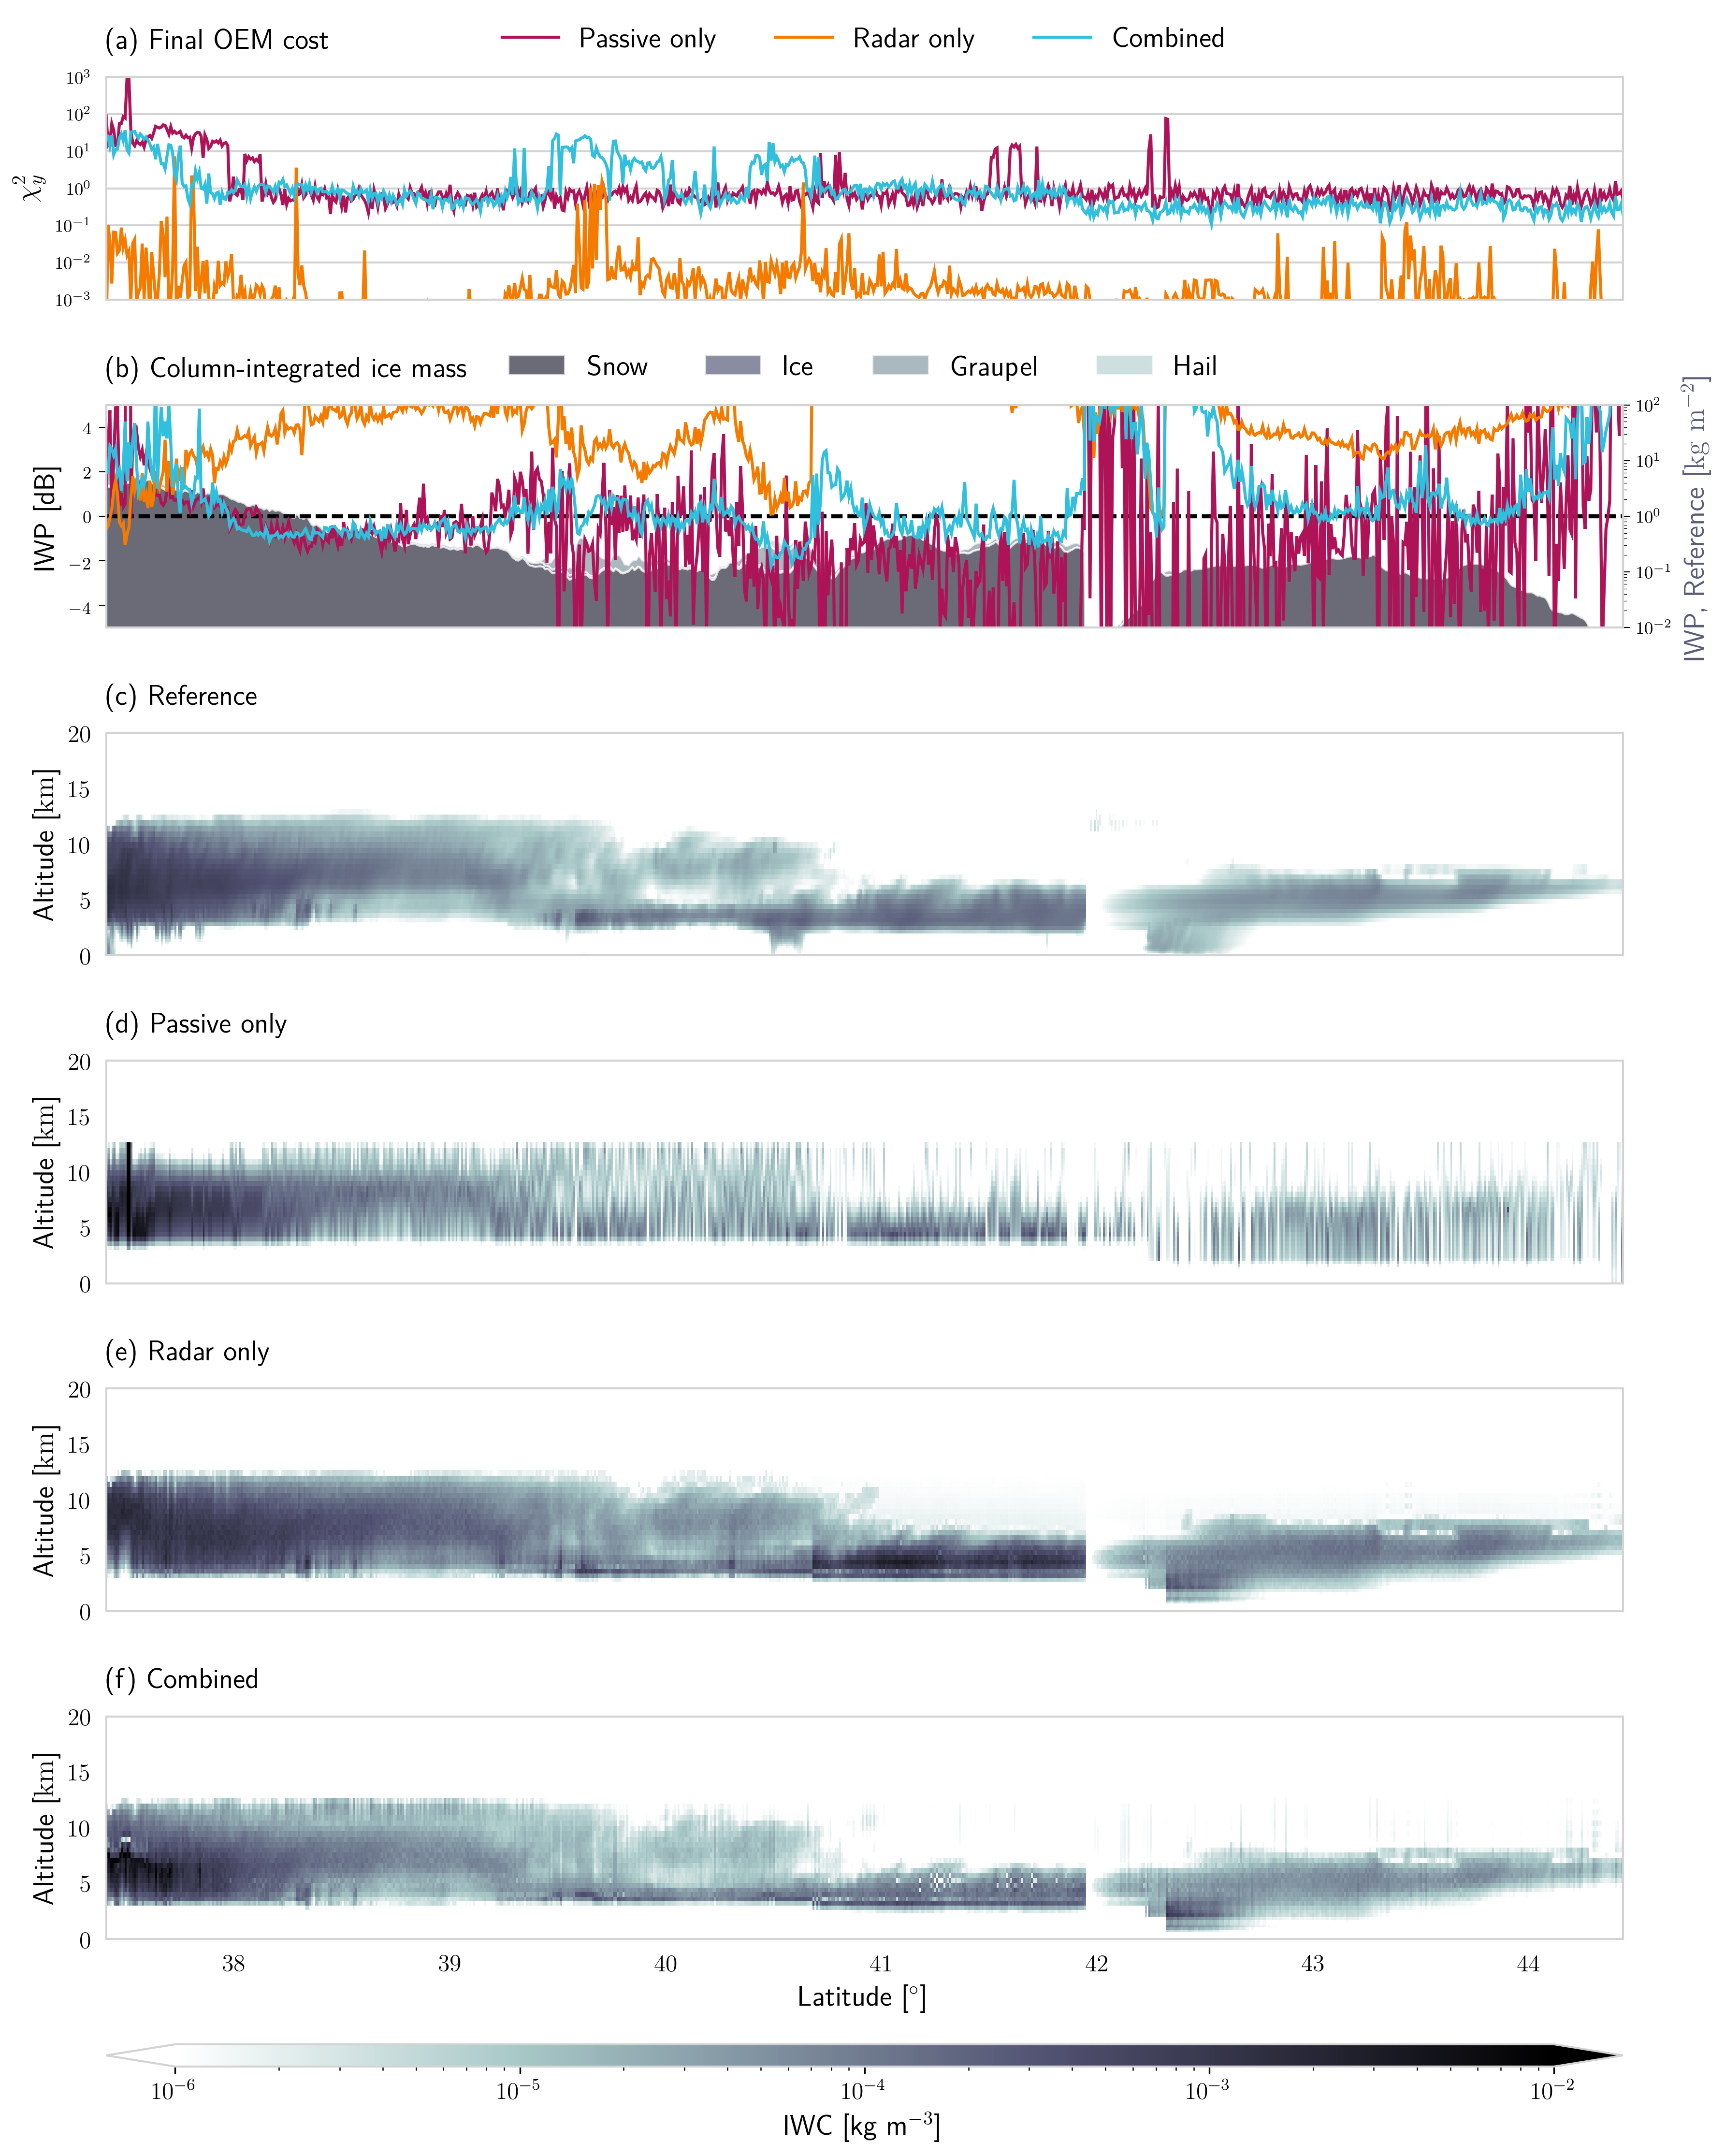
\includegraphics[width = 0.8\textwidth]{../plots/results_b_LargePlateAggregate}
\caption{\DIFaddFL{Results of the ice hydrometeor retrieval for the second test scene.
  Panel (a) displays the value of the $\chi^2_y$ diagnostic normalized by the
  dimension of the measurement space of the corresponding retrieval. Panel (b)
  shows retrieved IWP in dB relative to the reference IWP. Absolute reference
  IWP and the contributions from different hydrometeor classes are displayed by
  the filled areas in the background. Panel (c) displays the reference mass
  concentrations from the model scene. Panel (d), (e) and (f) display the
  retrieval results for the passive-only, radar-only and combined retrieval,
  respectively.}}
\label{fig:results_b}
\end{figure}

\begin{figure}[!h]
\centering
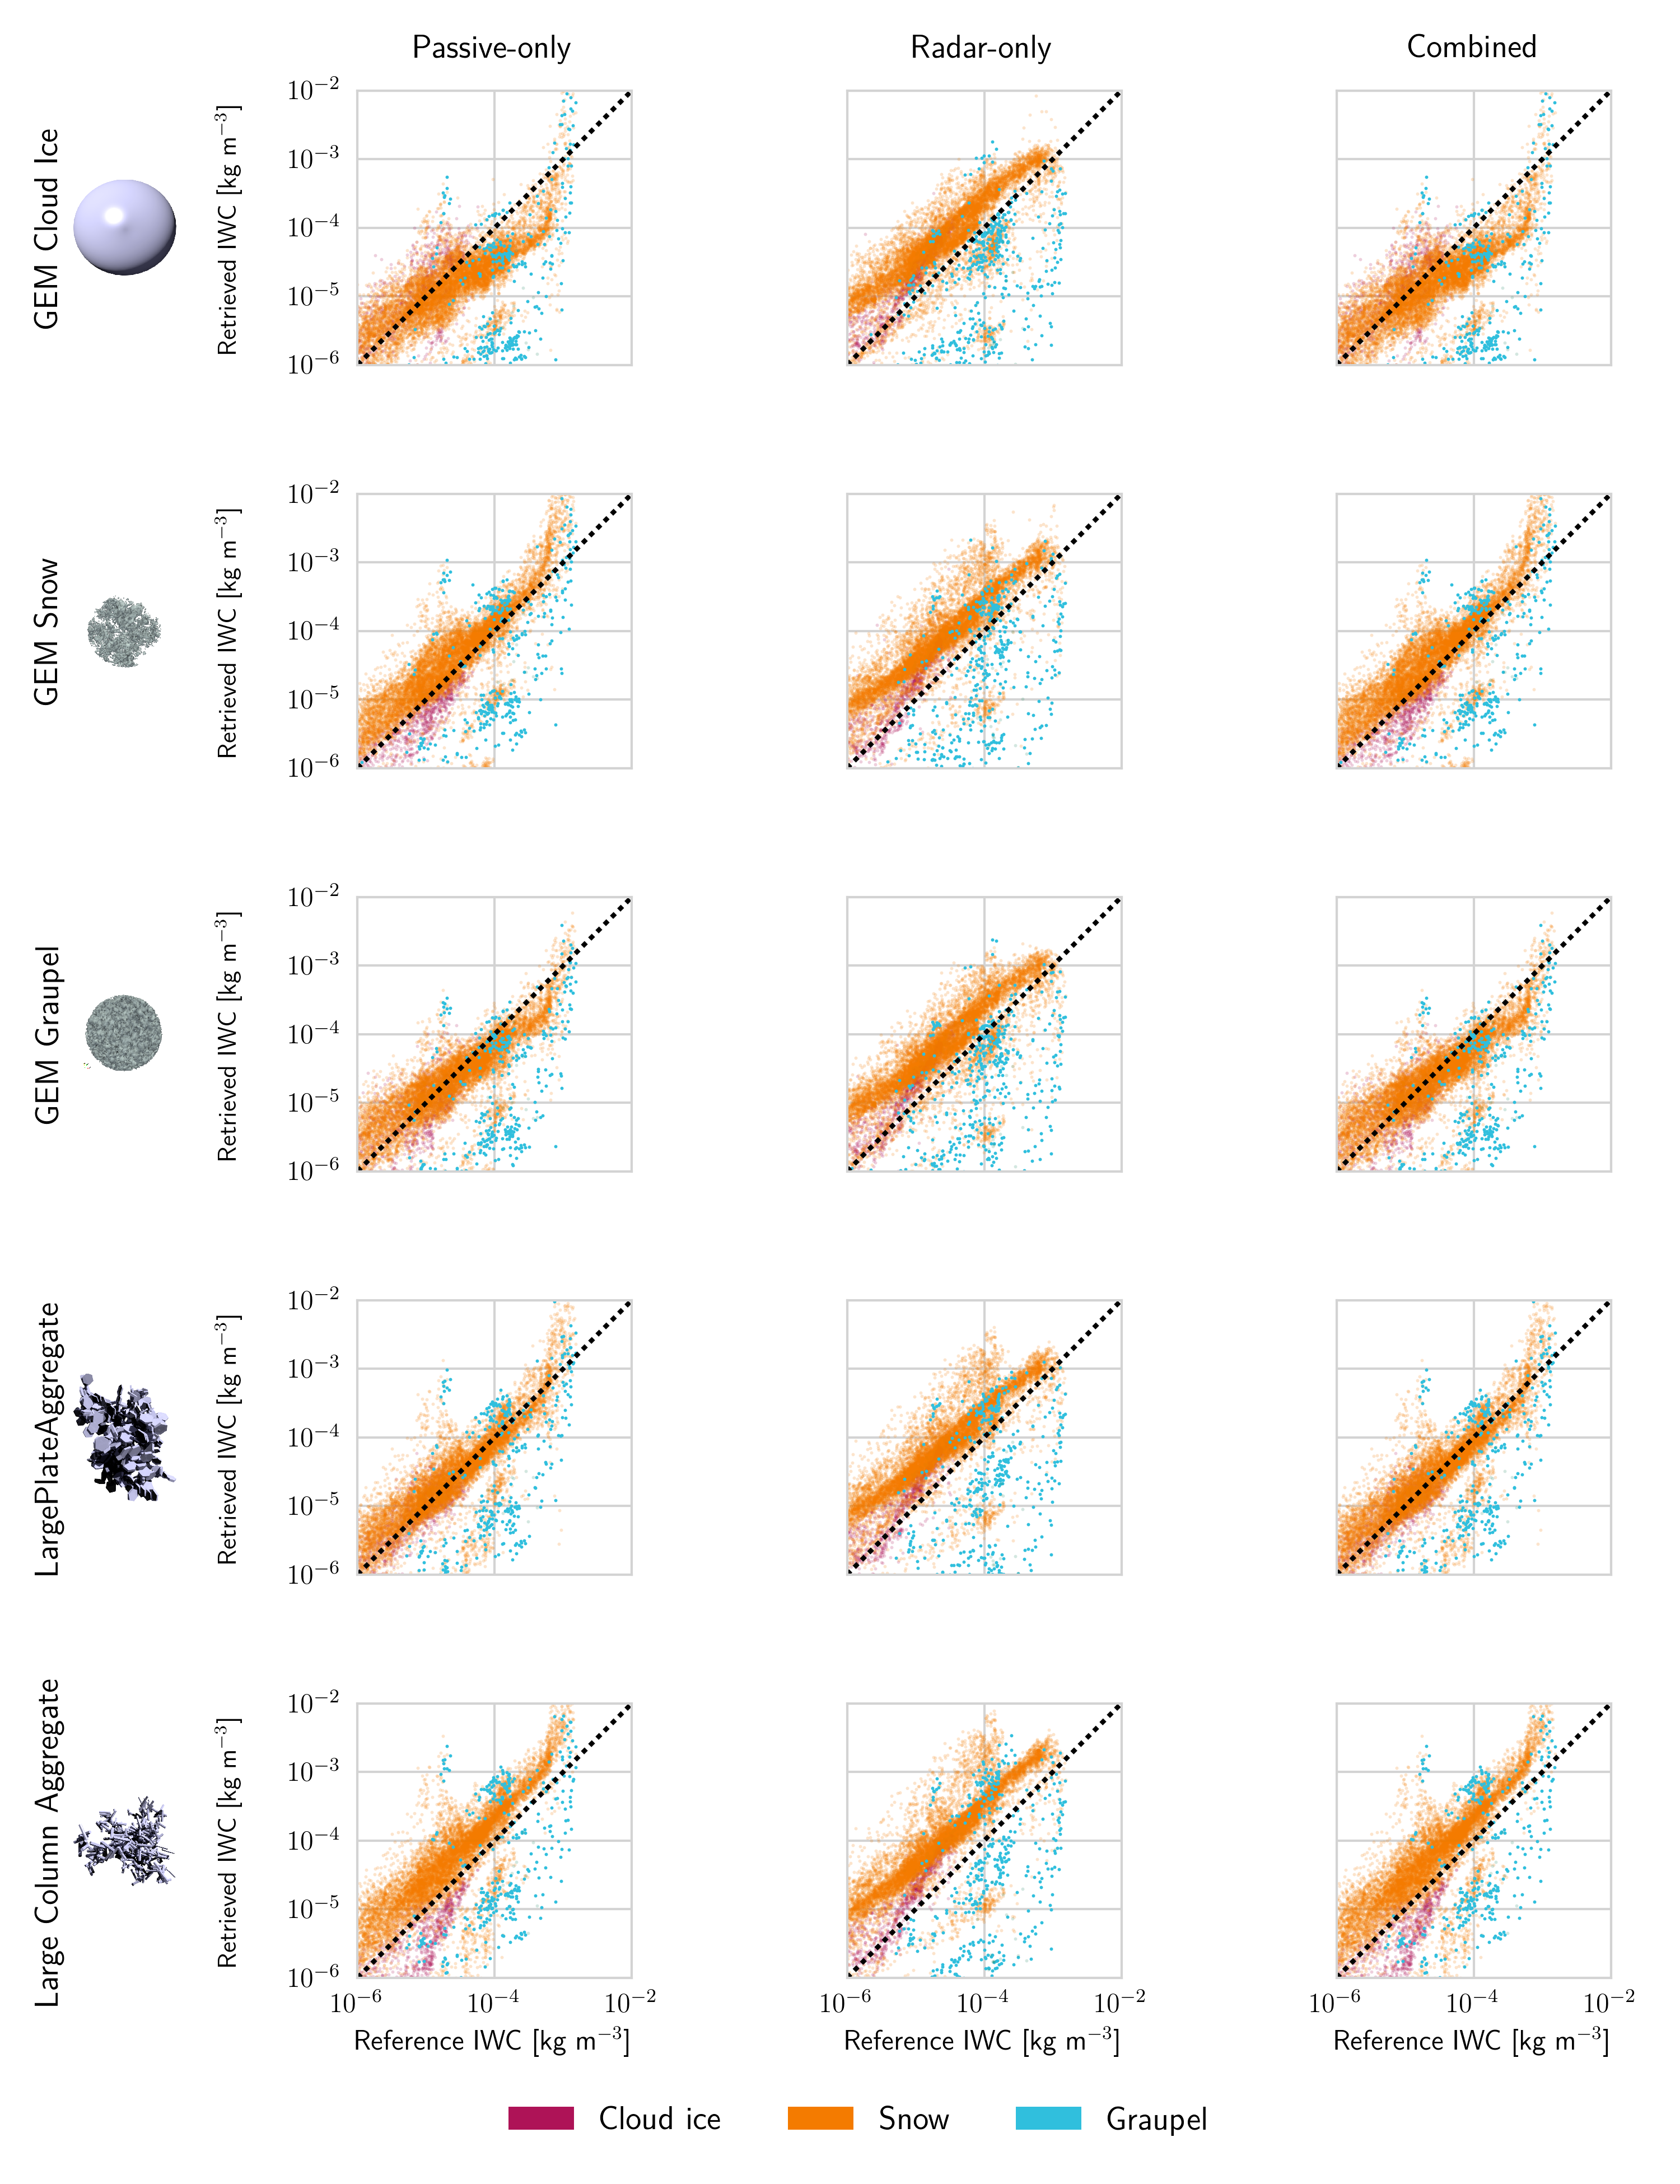
\includegraphics[width = 0.8\textwidth]{../plots/results_scatter_b}
\caption{\DIFaddFL{Scatter plots of the reference and retrieved IWC for
  the second test scene. The rows show the retrieval results for a given
  assumed ice particle model. The first column of each row displays a rendering
  of the particle model. The following rows display the results for the
  passive-only, the radar-only and the combined retrieval.}}
\label{fig:results_scatter_b}
\end{figure}

\clearpage
\DIFaddend 


%% Please add \clearpage between each table and/or figure. Further guidelines on figures and tables can be found below.

\DIFaddbegin \noappendix


\DIFaddend \authorcontribution{Simon Pfreundschuh has implemented the retrieval, performed
  the data analysis and written the manuscript. Patrick Eriksson and Richard
  Larsson have added code to the ARTS radiative transfer model that was required
  to perform the presented calculations. Stefan A. Buehler, Patrick Eriksson,
  Manfred Brath and Simon Pfreundschuh have collaborated on the study that lead
  to the results presented here. David Duncan and Robin Ekelund have contributed
  to the conceptualization of the study through comments and advice.}



\competinginterests{No competing interests are present.} %% this section is mandatory even if you declare that no competing interests are present

\begin{acknowledgements}

The combined and radar-only were developed as part of the ESA-funded study
``Scientific Concept Study for Wide-Swath High-Resolution Cloud Profiling''
(Contract number: 4000119850/17/NL/LvH). The authors would like to thank
study manager Tobias Wehr for his valuable input and guidance.

Furthermore, the authors would like to acknowledge the work of Zhipeng Qu,
Howard Barker, and Jason Cole from Environment and Climate Change Canada who
produced the model scenes that were used to test the retrieval.

The work of SP, PE and RE on this study was financially supported by the Swedish
National Space Agency (SNSA) under grants 150/14 and 166/18.

SB was supported by the Deutsche Forschungsgemeinschaft (DFG, German Research
Foundation) under Germany's Excellence Strategy --- EXC 2037 'Climate, Climatic
Change, and Society' --- Project Number: 390683824, contributing to the Center
for Earth System Research and Sustainability (CEN) of Universit\"{a}t Hamburg.

The computations for this study were performed using several freely available programming
languages and software packages, most prominently the Python language
\citep{python}, the IPython computing environment \citep{ipython}, the numpy
package for numerical computing \citep{numpy} and matplotlib for generating
figures \citep{matplotlib}\DIFaddbegin \DIFadd{.
}

\DIFadd{The computations were performed on resources at Chalmers Centre for
Computational Science and Engineering (C3SE) provided by the Swedish National
Infrastructure for Computing (SNIC)}\DIFaddend .

\end{acknowledgements}




%% REFERENCES

%% The reference list is compiled as follows:


%% Since the Copernicus LaTeX package includes the BibTeX style file copernicus.bst,
%% authors experienced with BibTeX only have to include the following two lines:

\bibliographystyle{copernicus}
\bibliography{references}
%%
%% URLs and DOIs can be entered in your BibTeX file as:
%%
%% URL = {http://www.xyz.org/~jones/idx_g.htm}
%% DOI = {10.5194/xyz}


%% LITERATURE CITATIONS
%%
%% command                        & example result
%% \citet{jones90}|               & Jones et al. (1990)
%% \citep{jones90}|               & (Jones et al., 1990)
%% \citep{jones90,jones93}|       & (Jones et al., 1990, 1993)
%% \citep[p.~32]{jones90}|        & (Jones et al., 1990, p.~32)
%% \citep[e.g.,][]{jones90}|      & (e.g., Jones et al., 1990)
%% \citep[e.g.,][p.~32]{jones90}| & (e.g., Jones et al., 1990, p.~32)
%% \citeauthor{jones90}|          & Jones et al.
%% \citeyear{jones90}|            & 1990



%% FIGURES

%% When figures and tables are placed at the end of the MS (article in one-column style), please add \clearpage
%% between bibliography and first table and/or figure as well as between each table and/or figure.


%% ONE-COLUMN FIGURES

%%f
%\begin{figure}[t]
%\includegraphics[width=8.3cm]{FILE NAME}
%\caption{TEXT}
%\end{figure}
%
%%% TWO-COLUMN FIGURES
%
%%f
%\begin{figure*}[t]
%\includegraphics[width=12cm]{FILE NAME}
%\caption{TEXT}
%\end{figure*}
%
%
%%% TABLES
%%%
%%% The different columns must be seperated with a & command and should
%%% end with \\ to identify the column brake.
%
%%% ONE-COLUMN TABLE
%
%%t
%\begin{table}[t]
%\caption{TEXT}
%\begin{tabular}{column = lcr}
%\tophline
%
%\middlehline
%
%\bottomhline
%\end{tabular}
%\belowtable{} % Table Footnotes
%\end{table}
%
%%% TWO-COLUMN TABLE
%
%%t
%\begin{table*}[t]
%\caption{TEXT}
%\begin{tabular}{column = lcr}
%\tophline
%
%\middlehline
%
%\bottomhline
%\end{tabular}
%\belowtable{} % Table Footnotes
%\end{table*}
%
%%% LANDSCAPE TABLE
%
%%t
%\begin{sidewaystable*}[t]
%\caption{TEXT}
%\begin{tabular}{column = lcr}
%\tophline
%
%\middlehline
%
%\bottomhline
%\end{tabular}
%\belowtable{} % Table Footnotes
%\end{sidewaystable*}
%
%
%%% MATHEMATICAL EXPRESSIONS
%
%%% All papers typeset by Copernicus Publications follow the math typesetting regulations
%%% given by the IUPAC Green Book (IUPAC: Quantities, Units and Symbols in Physical Chemistry,
%%% 2nd Edn., Blackwell Science, available at: http://old.iupac.org/publications/books/gbook/green_book_2ed.pdf, 1993).
%%%
%%% Physical quantities/variables are typeset in italic font (t for time, T for Temperature)
%%% Indices which are not defined are typeset in italic font (x, y, z, a, b, c)
%%% Items/objects which are defined are typeset in roman font (Car A, Car B)
%%% Descriptions/specifications which are defined by itself are typeset in roman font (abs, rel, ref, tot, net, ice)
%%% Abbreviations from 2 letters are typeset in roman font (RH, LAI)
%%% Vectors are identified in bold italic font using \vec{x}
%%% Matrices are identified in bold roman font
%%% Multiplication signs are typeset using the LaTeX commands \times (for vector products, grids, and exponential notations) or \cdot
%%% The character * should not be applied as mutliplication sign
%
%
%%% EQUATIONS
%
%%% Single-row equation
%
%\begin{equation}
%
%\end{equation}
%
%%% Multiline equation
%
%\begin{align}
%& 3 + 5 = 8\\
%& 3 + 5 = 8\\
%& 3 + 5 = 8
%\end{align}
%
%
%%% MATRICES
%
%\begin{matrix}
%x & y & z\\
%x & y & z\\
%x & y & z\\
%\end{matrix}
%
%
%%% ALGORITHM
%
%\begin{algorithm}
%\caption{...}
%\label{a1}
%\begin{algorithmic}
%...
%\end{algorithmic}
%\end{algorithm}
%
%
%%% CHEMICAL FORMULAS AND REACTIONS
%
%%% For formulas embedded in the text, please use \chem{}
%
%%% The reaction environment creates labels including the letter R, i.e. (R1), (R2), etc.
%
%\begin{reaction}
%%% \rightarrow should be used for normal (one-way) chemical reactions
%%% \rightleftharpoons should be used for equilibria
%%% \leftrightarrow should be used for resonance structures
%\end{reaction}
%
%
%%% PHYSICAL UNITS
%%%
%%% Please use \unit{} and apply the exponential notation


\end{document}
